%https://www.overleaf.com/learn/latex/Subscripts_and_superscripts
\RequirePackage[2020-02-02]{latexrelease}
\documentclass[14pt,fleqn]{extbook} % Default font size and left-justified equations
\usepackage{graphicx}
\usepackage{setspace}
\usepackage{graphicx} % Required for including pictures
\graphicspath{{Pictures/}} % Specifies the directory where pictures are stored

\usepackage{lipsum} % Inserts dummy text

\usepackage{tikz} % Required for drawing custom shapes

\usepackage[english]{babel} % English language/hyphenation

\usepackage{enumitem} % Customize lists
\setlist{nolistsep} % Reduce spacing between bullet points and numbered lists

\usepackage{booktabs} % Required for nicer horizontal rules in tables

\usepackage{xcolor} % Required for specifying colors by name
\definecolor{ocre}{RGB}{243,102,25} % Define the orange color used for highlighting throughout the book

%----------------------------------------------------------------------------------------
%	MARGINS
%----------------------------------------------------------------------------------------

\usepackage{geometry} % Required for adjusting page dimensions and margins

\geometry{
	paper=a4paper, % Paper size, change to letterpaper for US letter size
	top=3cm, % Top margin
	bottom=3cm, % Bottom margin
	left=3cm, % Left margin
	right=3cm, % Right margin
	headheight=14pt, % Header height
	footskip=1.4cm, % Space from the bottom margin to the baseline of the footer
	headsep=10pt, % Space from the top margin to the baseline of the header
	%showframe, % Uncomment to show how the type block is set on the page
}

%----------------------------------------------------------------------------------------
%	FONTS
%----------------------------------------------------------------------------------------

\usepackage{avant} % Use the Avantgarde font for headings
%\usepackage{times} % Use the Times font for headings
\usepackage{mathptmx} % Use the Adobe Times Roman as the default text font together with math symbols from the Sym­bol, Chancery and Com­puter Modern fonts

\usepackage{microtype} % Slightly tweak font spacing for aesthetics
\usepackage[utf8]{inputenc} % Required for including letters with accents
\usepackage[T1]{fontenc} % Use 8-bit encoding that has 256 glyphs

%----------------------------------------------------------------------------------------
%	BIBLIOGRAPHY AND INDEX
%----------------------------------------------------------------------------------------

\usepackage[style=numeric,citestyle=numeric,sorting=nyt,sortcites=true,autopunct=true,babel=hyphen,hyperref=true,abbreviate=false,backref=true,backend=biber]{biblatex}
\addbibresource{bibliography.bib} % BibTeX bibliography file
\defbibheading{bibempty}{}

\usepackage{calc} % For simpler calculation - used for spacing the index letter headings correctly
\usepackage{makeidx} % Required to make an index
\makeindex % Tells LaTeX to create the files required for indexing

%----------------------------------------------------------------------------------------
%	MAIN TABLE OF CONTENTS
%----------------------------------------------------------------------------------------

\usepackage{titletoc} % Required for manipulating the table of contents

\contentsmargin{0cm} % Removes the default margin

% Part text styling (this is mostly taken care of in the PART HEADINGS section of this file)
\titlecontents{part}
	[0cm] % Left indentation
	{\addvspace{20pt}\bfseries} % Spacing and font options for parts
	{}
	{}
	{}

% Chapter text styling
\titlecontents{chapter}
	[1.25cm] % Left indentation
	{\addvspace{12pt}\large\sffamily\bfseries} % Spacing and font options for chapters
	{\color{ocre!60}\contentslabel[\Large\thecontentslabel]{1.25cm}\color{ocre}} % Formatting of numbered sections of this type
	{\color{ocre}} % Formatting of numberless sections of this type
	{\color{ocre!60}\normalsize\;\titlerule*[.5pc]{.}\;\thecontentspage} % Formatting of the filler to the right of the heading and the page number

% Section text styling
\titlecontents{section}
	[1.25cm] % Left indentation
	{\addvspace{3pt}\sffamily\bfseries} % Spacing and font options for sections
	{\contentslabel[\thecontentslabel]{1.25cm}} % Formatting of numbered sections of this type
	{} % Formatting of numberless sections of this type
	{\hfill\color{black}\thecontentspage} % Formatting of the filler to the right of the heading and the page number

% Subsection text styling
\titlecontents{subsection}
	[1.25cm] % Left indentation
	{\addvspace{1pt}\sffamily\small} % Spacing and font options for subsections
	{\contentslabel[\thecontentslabel]{1.25cm}} % Formatting of numbered sections of this type
	{} % Formatting of numberless sections of this type
	{\ \titlerule*[.5pc]{.}\;\thecontentspage} % Formatting of the filler to the right of the heading and the page number

% Figure text styling
\titlecontents{figure}
	[1.25cm] % Left indentation
	{\addvspace{1pt}\sffamily\small} % Spacing and font options for figures
	{\thecontentslabel\hspace*{1em}} % Formatting of numbered sections of this type
	{} % Formatting of numberless sections of this type
	{\ \titlerule*[.5pc]{.}\;\thecontentspage} % Formatting of the filler to the right of the heading and the page number

% Table text styling
\titlecontents{table}
	[1.25cm] % Left indentation
	{\addvspace{1pt}\sffamily\small} % Spacing and font options for tables
	{\thecontentslabel\hspace*{1em}} % Formatting of numbered sections of this type
	{} % Formatting of numberless sections of this type
	{\ \titlerule*[.5pc]{.}\;\thecontentspage} % Formatting of the filler to the right of the heading and the page number

%----------------------------------------------------------------------------------------
%	MINI TABLE OF CONTENTS IN PART HEADS
%----------------------------------------------------------------------------------------

% Chapter text styling
\titlecontents{lchapter}
	[0em] % Left indentation
	{\addvspace{15pt}\large\sffamily\bfseries} % Spacing and font options for chapters
	{\color{ocre}\contentslabel[\Large\thecontentslabel]{1.25cm}\color{ocre}} % Chapter number
	{}  
	{\color{ocre}\normalsize\sffamily\bfseries\;\titlerule*[.5pc]{.}\;\thecontentspage} % Page number

% Section text styling
\titlecontents{lsection}
	[0em] % Left indentation
	{\sffamily\small} % Spacing and font options for sections
	{\contentslabel[\thecontentslabel]{1.25cm}} % Section number
	{}
	{}

% Subsection text styling (note these aren't shown by default, display them by searchings this file for tocdepth and reading the commented text)
\titlecontents{lsubsection}
	[.5em] % Left indentation
	{\sffamily\footnotesize} % Spacing and font options for subsections
	{\contentslabel[\thecontentslabel]{1.25cm}}
	{}
	{}

%----------------------------------------------------------------------------------------
%	HEADERS AND FOOTERS
%----------------------------------------------------------------------------------------

\usepackage{fancyhdr} % Required for header and footer configuration

\pagestyle{fancy} % Enable the custom headers and footers

\renewcommand{\chaptermark}[1]{\markboth{\sffamily\normalsize\bfseries\chaptername\ \thechapter.\ #1}{}} % Styling for the current chapter in the header
\renewcommand{\sectionmark}[1]{\markright{\sffamily\normalsize\thesection\hspace{5pt}#1}{}} % Styling for the current section in the header

\fancyhf{} % Clear default headers and footers
\fancyhead[LE,RO]{\sffamily\normalsize\thepage} % Styling for the page number in the header
\fancyhead[LO]{\rightmark} % Print the nearest section name on the left side of odd pages
\fancyhead[RE]{\leftmark} % Print the current chapter name on the right side of even pages
%\fancyfoot[C]{\thepage} % Uncomment to include a footer

\renewcommand{\headrulewidth}{0.5pt} % Thickness of the rule under the header

\fancypagestyle{plain}{% Style for when a plain pagestyle is specified
	\fancyhead{}\renewcommand{\headrulewidth}{0pt}%
}

% Removes the header from odd empty pages at the end of chapters
\makeatletter
\renewcommand{\cleardoublepage}{
\clearpage\ifodd\c@page\else
\hbox{}
\vspace*{\fill}
\thispagestyle{empty}
\newpage
\fi}

%----------------------------------------------------------------------------------------
%	THEOREM STYLES
%----------------------------------------------------------------------------------------

\usepackage{amsmath,amsfonts,amssymb,amsthm} % For math equations, theorems, symbols, etc

\newcommand{\intoo}[2]{\mathopen{]}#1\,;#2\mathclose{[}}
\newcommand{\ud}{\mathop{\mathrm{{}d}}\mathopen{}}
\newcommand{\intff}[2]{\mathopen{[}#1\,;#2\mathclose{]}}
\renewcommand{\qedsymbol}{$\blacksquare$}
\newtheorem{notation}{Notation}[chapter]

% Boxed/framed environments
\newtheoremstyle{ocrenumbox}% Theorem style name
{0pt}% Space above
{0pt}% Space below
{\normalfont}% Body font
{}% Indent amount
{\small\bf\sffamily\color{ocre}}% Theorem head font
{\;}% Punctuation after theorem head
{0.25em}% Space after theorem head
{\small\sffamily\color{ocre}\thmname{#1}\nobreakspace\thmnumber{\@ifnotempty{#1}{}\@upn{#2}}% Theorem text (e.g. Theorem 2.1)
\thmnote{\nobreakspace\the\thm@notefont\sffamily\bfseries\color{black}---\nobreakspace#3.}} % Optional theorem note

\newtheoremstyle{blacknumex}% Theorem style name
{5pt}% Space above
{5pt}% Space below
{\normalfont}% Body font
{} % Indent amount
{\small\bf\sffamily}% Theorem head font
{\;}% Punctuation after theorem head
{0.25em}% Space after theorem head
{\small\sffamily{\tiny\ensuremath{\blacksquare}}\nobreakspace\thmname{#1}\nobreakspace\thmnumber{\@ifnotempty{#1}{}\@upn{#2}}% Theorem text (e.g. Theorem 2.1)
\thmnote{\nobreakspace\the\thm@notefont\sffamily\bfseries---\nobreakspace#3.}}% Optional theorem note

\newtheoremstyle{blacknumbox} % Theorem style name
{0pt}% Space above
{0pt}% Space below
{\normalfont}% Body font
{}% Indent amount
{\small\bf\sffamily}% Theorem head font
{\;}% Punctuation after theorem head
{0.25em}% Space after theorem head
{\small\sffamily\thmname{#1}\nobreakspace\thmnumber{\@ifnotempty{#1}{}\@upn{#2}}% Theorem text (e.g. Theorem 2.1)
\thmnote{\nobreakspace\the\thm@notefont\sffamily\bfseries---\nobreakspace#3.}}% Optional theorem note

% Non-boxed/non-framed environments
\newtheoremstyle{ocrenum}% Theorem style name
{5pt}% Space above
{5pt}% Space below
{\normalfont}% Body font
{}% Indent amount
{\small\bf\sffamily\color{ocre}}% Theorem head font
{\;}% Punctuation after theorem head
{0.25em}% Space after theorem head
{\small\sffamily\color{ocre}\thmname{#1}\nobreakspace\thmnumber{\@ifnotempty{#1}{}\@upn{#2}}% Theorem text (e.g. Theorem 2.1)
\thmnote{\nobreakspace\the\thm@notefont\sffamily\bfseries\color{black}---\nobreakspace#3.}} % Optional theorem note
\makeatother

% Defines the theorem text style for each type of theorem to one of the three styles above
\newcounter{dummy} 
\numberwithin{dummy}{section}
\theoremstyle{ocrenumbox}
\newtheorem{theoremeT}[dummy]{Theorem}
\newtheorem{problem}{Problem}[chapter]
\newtheorem{exerciseT}{Exercise}[chapter]
\theoremstyle{blacknumex}
\newtheorem{exampleT}{Example}[chapter]
\theoremstyle{blacknumbox}
\newtheorem{vocabulary}{Vocabulary}[chapter]
\newtheorem{definitionT}{Definition}[section]
\newtheorem{corollaryT}[dummy]{Corollary}
\theoremstyle{ocrenum}
\newtheorem{proposition}[dummy]{Proposition}

%----------------------------------------------------------------------------------------
%	DEFINITION OF COLORED BOXES
%----------------------------------------------------------------------------------------

\RequirePackage[framemethod=default]{mdframed} % Required for creating the theorem, definition, exercise and corollary boxes

% Theorem box
\newmdenv[skipabove=7pt,
skipbelow=7pt,
backgroundcolor=black!5,
linecolor=ocre,
innerleftmargin=5pt,
innerrightmargin=5pt,
innertopmargin=5pt,
leftmargin=0cm,
rightmargin=0cm,
innerbottommargin=5pt]{tBox}

% Exercise box	  
\newmdenv[skipabove=7pt,
skipbelow=7pt,
rightline=false,
leftline=true,
topline=false,
bottomline=false,
backgroundcolor=ocre!10,
linecolor=ocre,
innerleftmargin=5pt,
innerrightmargin=5pt,
innertopmargin=5pt,
innerbottommargin=5pt,
leftmargin=0cm,
rightmargin=0cm,
linewidth=4pt]{eBox}	

% Definition box
\newmdenv[skipabove=7pt,
skipbelow=7pt,
rightline=false,
leftline=true,
topline=false,
bottomline=false,
linecolor=ocre,
innerleftmargin=5pt,
innerrightmargin=5pt,
innertopmargin=0pt,
leftmargin=0cm,
rightmargin=0cm,
linewidth=4pt,
innerbottommargin=0pt]{dBox}	

% Corollary box
\newmdenv[skipabove=7pt,
skipbelow=7pt,
rightline=false,
leftline=true,
topline=false,
bottomline=false,
linecolor=gray,
backgroundcolor=black!5,
innerleftmargin=5pt,
innerrightmargin=5pt,
innertopmargin=5pt,
leftmargin=0cm,
rightmargin=0cm,
linewidth=4pt,
innerbottommargin=5pt]{cBox}

% Creates an environment for each type of theorem and assigns it a theorem text style from the "Theorem Styles" section above and a colored box from above
\newenvironment{theorem}{\begin{tBox}\begin{theoremeT}}{\end{theoremeT}\end{tBox}}
\newenvironment{exercise}{\begin{eBox}\begin{exerciseT}}{\hfill{\color{ocre}\tiny\ensuremath{\blacksquare}}\end{exerciseT}\end{eBox}}				  
\newenvironment{definition}{\begin{dBox}\begin{definitionT}}{\end{definitionT}\end{dBox}}	
\newenvironment{example}{\begin{exampleT}}{\hfill{\tiny\ensuremath{\blacksquare}}\end{exampleT}}		
\newenvironment{corollary}{\begin{cBox}\begin{corollaryT}}{\end{corollaryT}\end{cBox}}	

%----------------------------------------------------------------------------------------
%	REMARK ENVIRONMENT
%----------------------------------------------------------------------------------------

\newenvironment{remark}{\par\vspace{10pt}\small % Vertical white space above the remark and smaller font size
\begin{list}{}{
\leftmargin=35pt % Indentation on the left
\rightmargin=25pt}\item\ignorespaces % Indentation on the right
\makebox[-2.5pt]{\begin{tikzpicture}[overlay]
\node[draw=ocre!60,line width=1pt,circle,fill=ocre!25,font=\sffamily\bfseries,inner sep=2pt,outer sep=0pt] at (-15pt,0pt){\textcolor{ocre}{R}};\end{tikzpicture}} % Orange R in a circle
\advance\baselineskip -1pt}{\end{list}\vskip5pt} % Tighter line spacing and white space after remark

%----------------------------------------------------------------------------------------
%	SECTION NUMBERING IN THE MARGIN
%----------------------------------------------------------------------------------------

\makeatletter
\renewcommand{\@seccntformat}[1]{\llap{\textcolor{ocre}{\csname the#1\endcsname}\hspace{1em}}}                    
\renewcommand{\section}{\@startsection{section}{1}{\z@}
{-4ex \@plus -1ex \@minus -.4ex}
{1ex \@plus.2ex }
{\normalfont\large\sffamily\bfseries}}
\renewcommand{\subsection}{\@startsection {subsection}{2}{\z@}
{-3ex \@plus -0.1ex \@minus -.4ex}
{0.5ex \@plus.2ex }
{\normalfont\sffamily\bfseries}}
\renewcommand{\subsubsection}{\@startsection {subsubsection}{3}{\z@}
{-2ex \@plus -0.1ex \@minus -.2ex}
{.2ex \@plus.2ex }
{\normalfont\small\sffamily\bfseries}}                        
\renewcommand\paragraph{\@startsection{paragraph}{4}{\z@}
{-2ex \@plus-.2ex \@minus .2ex}
{.1ex}
{\normalfont\small\sffamily\bfseries}}

%----------------------------------------------------------------------------------------
%	PART HEADINGS
%----------------------------------------------------------------------------------------

% Numbered part in the table of contents
\newcommand{\@mypartnumtocformat}[2]{%
	\setlength\fboxsep{0pt}%
	\noindent\colorbox{ocre!20}{\strut\parbox[c][.7cm]{\ecart}{\color{ocre!70}\Large\sffamily\bfseries\centering#1}}\hskip\esp\colorbox{ocre!40}{\strut\parbox[c][.7cm]{\linewidth-\ecart-\esp}{\Large\sffamily\centering#2}}%
}

% Unnumbered part in the table of contents
\newcommand{\@myparttocformat}[1]{%
	\setlength\fboxsep{0pt}%
	\noindent\colorbox{ocre!40}{\strut\parbox[c][.7cm]{\linewidth}{\Large\sffamily\centering#1}}%
}

\newlength\esp
\setlength\esp{4pt}
\newlength\ecart
\setlength\ecart{1.2cm-\esp}
\newcommand{\thepartimage}{}%
\newcommand{\partimage}[1]{\renewcommand{\thepartimage}{#1}}%
\def\@part[#1]#2{%
\ifnum \c@secnumdepth >-2\relax%
\refstepcounter{part}%
\addcontentsline{toc}{part}{\texorpdfstring{\protect\@mypartnumtocformat{\thepart}{#1}}{\partname~\thepart\ ---\ #1}}
\else%
\addcontentsline{toc}{part}{\texorpdfstring{\protect\@myparttocformat{#1}}{#1}}%
\fi%
\startcontents%
\markboth{}{}%
{\thispagestyle{empty}%
\begin{tikzpicture}[remember picture,overlay]%
\node at (current page.north west){\begin{tikzpicture}[remember picture,overlay]%	
\fill[ocre!20](0cm,0cm) rectangle (\paperwidth,-\paperheight);
\node[anchor=north] at (4cm,-3.25cm){\color{ocre!40}\fontsize{220}{100}\sffamily\bfseries\thepart}; 
\node[anchor=south east] at (\paperwidth-1cm,-\paperheight+1cm){\parbox[t][][t]{8.5cm}{
\printcontents{l}{0}{\setcounter{tocdepth}{1}}% The depth to which the Part mini table of contents displays headings; 0 for chapters only, 1 for chapters and sections and 2 for chapters, sections and subsections
}};
\node[anchor=north east] at (\paperwidth-1.5cm,-3.25cm){\parbox[t][][t]{15cm}{\strut\raggedleft\color{white}\fontsize{30}{30}\sffamily\bfseries#2}};
\end{tikzpicture}};
\end{tikzpicture}}%
\@endpart}
\def\@spart#1{%
\startcontents%
\phantomsection
{\thispagestyle{empty}%
\begin{tikzpicture}[remember picture,overlay]%
\node at (current page.north west){\begin{tikzpicture}[remember picture,overlay]%	
\fill[ocre!20](0cm,0cm) rectangle (\paperwidth,-\paperheight);
\node[anchor=north east] at (\paperwidth-1.5cm,-3.25cm){\parbox[t][][t]{15cm}{\strut\raggedleft\color{white}\fontsize{30}{30}\sffamily\bfseries#1}};
\end{tikzpicture}};
\end{tikzpicture}}
\addcontentsline{toc}{part}{\texorpdfstring{%
\setlength\fboxsep{0pt}%
\noindent\protect\colorbox{ocre!40}{\strut\protect\parbox[c][.7cm]{\linewidth}{\Large\sffamily\protect\centering #1\quad\mbox{}}}}{#1}}%
\@endpart}
\def\@endpart{\vfil\newpage
\if@twoside
\if@openright
\null
\thispagestyle{empty}%
\newpage
\fi
\fi
\if@tempswa
\twocolumn
\fi}

%----------------------------------------------------------------------------------------
%	CHAPTER HEADINGS
%----------------------------------------------------------------------------------------

% A switch to conditionally include a picture, implemented by Christian Hupfer
\newif\ifusechapterimage
\usechapterimagetrue
\newcommand{\thechapterimage}{}%
\newcommand{\chapterimage}[1]{\ifusechapterimage\renewcommand{\thechapterimage}{#1}\fi}%
\newcommand{\autodot}{.}
\def\@makechapterhead#1{%
{\parindent \z@ \raggedright \normalfont
\ifnum \c@secnumdepth >\m@ne
\if@mainmatter
\begin{tikzpicture}[remember picture,overlay]
\node at (current page.north west)
{\begin{tikzpicture}[remember picture,overlay]
\node[anchor=north west,inner sep=0pt] at (0,0) {\ifusechapterimage\includegraphics[width=\paperwidth]{\thechapterimage}\fi};
\draw[anchor=west] (\Gm@lmargin,-9cm) node [line width=2pt,rounded corners=15pt,draw=ocre,fill=white,fill opacity=0.5,inner sep=15pt]{\strut\makebox[22cm]{}};
\draw[anchor=west] (\Gm@lmargin+.3cm,-9cm) node {\huge\sffamily\bfseries\color{black}\thechapter\autodot~#1\strut};
\end{tikzpicture}};
\end{tikzpicture}
\else
\begin{tikzpicture}[remember picture,overlay]
\node at (current page.north west)
{\begin{tikzpicture}[remember picture,overlay]
\node[anchor=north west,inner sep=0pt] at (0,0) {\ifusechapterimage\includegraphics[width=\paperwidth]{\thechapterimage}\fi};
\draw[anchor=west] (\Gm@lmargin,-9cm) node [line width=2pt,rounded corners=15pt,draw=ocre,fill=white,fill opacity=0.5,inner sep=15pt]{\strut\makebox[22cm]{}};
\draw[anchor=west] (\Gm@lmargin+.3cm,-9cm) node {\huge\sffamily\bfseries\color{black}#1\strut};
\end{tikzpicture}};
\end{tikzpicture}
\fi\fi\par\vspace*{270\p@}}}

%-------------------------------------------

\def\@makeschapterhead#1{%
\begin{tikzpicture}[remember picture,overlay]
\node at (current page.north west)
{\begin{tikzpicture}[remember picture,overlay]
\node[anchor=north west,inner sep=0pt] at (0,0) {\ifusechapterimage\includegraphics[width=\paperwidth]{\thechapterimage}\fi};
\draw[anchor=west] (\Gm@lmargin,-9cm) node [line width=2pt,rounded corners=15pt,draw=ocre,fill=white,fill opacity=0.5,inner sep=15pt]{\strut\makebox[22cm]{}};
\draw[anchor=west] (\Gm@lmargin+.3cm,-9cm) node {\huge\sffamily\bfseries\color{black}#1\strut};
\end{tikzpicture}};
\end{tikzpicture}
\par\vspace*{270\p@}}
\makeatother

%----------------------------------------------------------------------------------------
%	LINKS
%----------------------------------------------------------------------------------------

\usepackage{hyperref}
\hypersetup{hidelinks,backref=true,pagebackref=true,hyperindex=true,colorlinks=false,breaklinks=true,urlcolor=ocre,bookmarks=true,bookmarksopen=false}

\usepackage{bookmark}
\bookmarksetup{
open,
numbered,
addtohook={%
\ifnum\bookmarkget{level}=0 % chapter
\bookmarksetup{bold}%
\fi
\ifnum\bookmarkget{level}=-1 % part
\bookmarksetup{color=ocre,bold}%
\fi
}
}
 % Insert the commands.tex file which contains the majority of the structure behind the template
\usepackage{color}
\usepackage[utf8]{inputenc}
\definecolor{light}{rgb}{0.5, 0.5, 0.5}
\definecolor{back}{RGB}{245, 214, 235}
\definecolor{sborder}{RGB}{255, 230, 234}
\definecolor{scontent}{RGB}{255, 191, 191}
\definecolor{oborder}{RGB}{214, 245, 214}
\definecolor{ocontent}{RGB}{148, 201, 115}
\definecolor{eborder}{RGB}{255, 153, 153}
\definecolor{econtent}{RGB}{255, 0, 0}
\definecolor{ans}{RGB}{242, 242, 242}
\def\light#1{{\color{light}#1}}
\usepackage{multicol}
\usepackage{parskip}
\usepackage{fancyhdr}
\usepackage{tabulary}
\usepackage{adjustbox}
\usepackage{subfig}
\usepackage{xcolor}
\usepackage{tcolorbox}
\usepackage{amssymb}
\usepackage{afterpage}

\tcbuselibrary{breakable}
\usepackage[printwatermark]{xwatermark}
\usepackage{multirow}
% tickmarks and wrong mark
\usepackage{amssymb}% http://ctan.org/pkg/amssymb
\usepackage{pifont}% http://ctan.org/pkg/pifont
\newcommand{\cmark}{\ding{51}}%
\newcommand{\xmark}{\ding{55}}%
\definecolor{ncontent}{RGB}{255, 242, 0}
\definecolor{nborder}{RGB}{255, 255, 179}

\definecolor{border}{RGB}{245,245,245}

\newcommand\blankpage{%
	\null
	\thispagestyle{empty}%
	\addtocounter{page}{-1}%
	\newpage}

\fancyfoot[R]
{
	
\includegraphics[scale=0.6]{content/logo.png}%
}


\usepackage{framed}


\newcommand{\codeblockfull}[2] {
	\begin{tcolorbox}[
		space to upper,
		colback=white,
		collower=white,
		title=\textbf{#1},
		coltitle = white,]
		\color{black}
		\fontdimen2\font=8pt
		#2
		\fontdimen2\font=4pt
	\end{tcolorbox}
}

\newcommand{\codeblock}[1] {
	\begin{tcolorbox}[
		space to upper,
		colback=white,
		collower=white,
		title=\textbf{Code:},
		coltitle = white,]
		\color{black}
		\fontdimen2\font=8pt
		#1
		\fontdimen2\font=4pt
	\end{tcolorbox}
}



\newcommand{\codecontinue}[1] {
	\begin{tcolorbox}[
		space to upper,
		colback=white,
		collower=white,
		coltitle = white,]
		\color{black}
		\fontdimen2\font=8pt
		#1
		\fontdimen2\font=4pt
	\end{tcolorbox}
}



\newcommand{\datablock}[1] {
	\begin{tcolorbox}[
		space to upper,
		colback=white,
		collower=white,
		title=\textbf{Dataset:},
		coltitle = white,]
		\color{black}
		\fontdimen2\font=8pt
		#1
		\fontdimen2\font=4pt
	\end{tcolorbox}
}


\newcommand{\syntaxblock}[1] {
	\begin{tcolorbox}[
		space to upper,
		colback=scontent,
		title=\textbf{Syntax:},
		colframe=sborder,
		coltitle = black,]
		\color{black}
		\fontdimen2\font=8pt
		#1
		\fontdimen2\font=4pt
	\end{tcolorbox}
}


\newcommand{\noteblock}[1] {
	\begin{tcolorbox}[
		space to upper,
		colback=ncontent,
		title=\textbf{Note:},
		colframe=nborder,
		coltitle = black,]
		\color{black}
		\fontdimen2\font=8pt
		#1
		\fontdimen2\font=4pt
	\end{tcolorbox}
}


\newcommand{\outputblock}[1] {
	\begin{tcolorbox}[
		space to upper,
		colback=ocontent,
		title=\textbf{Query:},
		colframe=oborder,
		coltitle = black,]
		\color{black}
		\fontdimen2\font=8pt
		#1
		\fontdimen2\font=4pt
	\end{tcolorbox}
}

\newcommand{\errorblock}[1] {
	\begin{tcolorbox}[
		space to upper,
		colback=econtent,
		title=\textbf{Error:},
		colframe=eborder,
		coltitle = black,]
		\color{black}
		\fontdimen2\font=8pt
		#1
		\fontdimen2\font=4pt
	\end{tcolorbox}
}

\newcommand{\n} {
	\newline
}

\newcommand{\boximage}[2] {
	\includegraphics[width=#1\textwidth]{#2}
}


\newcommand{\s} {
	\hphantom{} \hphantom{} \hphantom{}
}

\newcommand{\bspace} {
	\bigskip
}

\newcommand{\tabletwo}[1] {
	\bspace
	\begin{tabular}{ |p{7cm}|p{7cm}| }
		\hline
		#1
		\hline
	\end{tabular}
}

\newcommand{\tableinsidebox}[1] {
	\bspace
	\begin{tabular}{ |p{6cm}|p{6cm}| }
		\hline
		#1
		\hline
	\end{tabular}
}

\newcommand{\commandblock}[1] {
	\begin{tcolorbox}[
		space to upper,
		colback=white,
		collower=white,
		title=\textbf{Query:},
		coltitle = white,]
		\color{black}
		\fontdimen2\font=8pt
		#1
		\fontdimen2\font=4pt
	\end{tcolorbox}
}

\newcommand{\tablethree}[1] {
	\bspace
	\begin{tabular}{ |p{4cm}|p{4cm}|p{4cm}| }
		\hline
		#1
		\hline
	\end{tabular}
}


\newcommand{\tablefour}[1] {
	\bspace
	\begin{tabular}{ |p{3.5cm}|p{3.5cm}|p{3.5cm}|p{3.5cm}| }
		\hline
		#1
		\hline
	\end{tabular}
}

\newcommand{\error}[1] {
	\color{red}\# Error: \newline
	#1 \color{black}
}

\newcommand{\ecode}[1] {
	\color{red}
	#1 \color{black}
}


\newcommand{\correct}[1] {
	\color{correctans}\# Output: \newline
	#1 \color{black}
}

\newcommand{\answer}[1] {
	
	\begin{tcolorbox}[space to upper,
		colback=ans,
		collower=white,
		coltitle = black, 
		colframe=border,
		title={Answer:},]
		#1
	\end{tcolorbox}
}

\newcommand{\quest}[2] {
	\begin{tcolorbox}[space to upper,
		colback=ans,
		collower=white,
		coltitle = white, 
		title={\textbf{#1}},]
		Ans: #2
	\end{tcolorbox}
}

\newcommand{\anscontinue}[1] {
	\begin{tcolorbox}
		#1
	\end{tcolorbox}
}

\newcommand{\newimage}[2] {
	\begin{figure}[h!]
		\centering
		\includegraphics[scale=#1]{#2}
	\end{figure}			
}

\thispagestyle{plain}
%\hypersetup{pdftitle={Title},pdfauthor={Author}} % Uncomment and fill out to include PDF metadata for the author and title of the book

%----------------------------------------------------------------------------------------
\setstretch{1.25}
%\definecolor[new][h=9A957A, a=1, t=.3]
\definecolor{code}{RGB}{248,248,248}
\definecolor{output}{RGB}{148, 201, 115}
\definecolor{error}{RGB}{255, 77, 77}
\definecolor{trick}{RGB}{242, 204, 255}
%%%%%%%%%%%%%%%%%%%%%%%   This block adds watermark  %%%%%%%%%%%%%%%%%
%\newsavebox\mybox
%\savebox\mybox{\tikz[color=mycolor,opacity=0.2]\node{lavatechtechnology.com};}
%\newwatermark*[
%allpages,
%angle=45,
%scale=2.5,
%xpos=-20,
%ypos=15
%]{\usebox\mybox}
%%%%%%%%%%%%%%%%%%%%%%%   This block adds watermark  %%%%%%%%%%%%%%%%%



\begin{document}

%----------------------------------------------------------------------------------------
%	TITLE PAGE
%----------------------------------------------------------------------------------------

\begingroup
\thispagestyle{empty} % Suppress headers and footers on the title page
\begin{tikzpicture}[remember picture,overlay]
\node[inner sep=0pt] (background) at (current page.center) {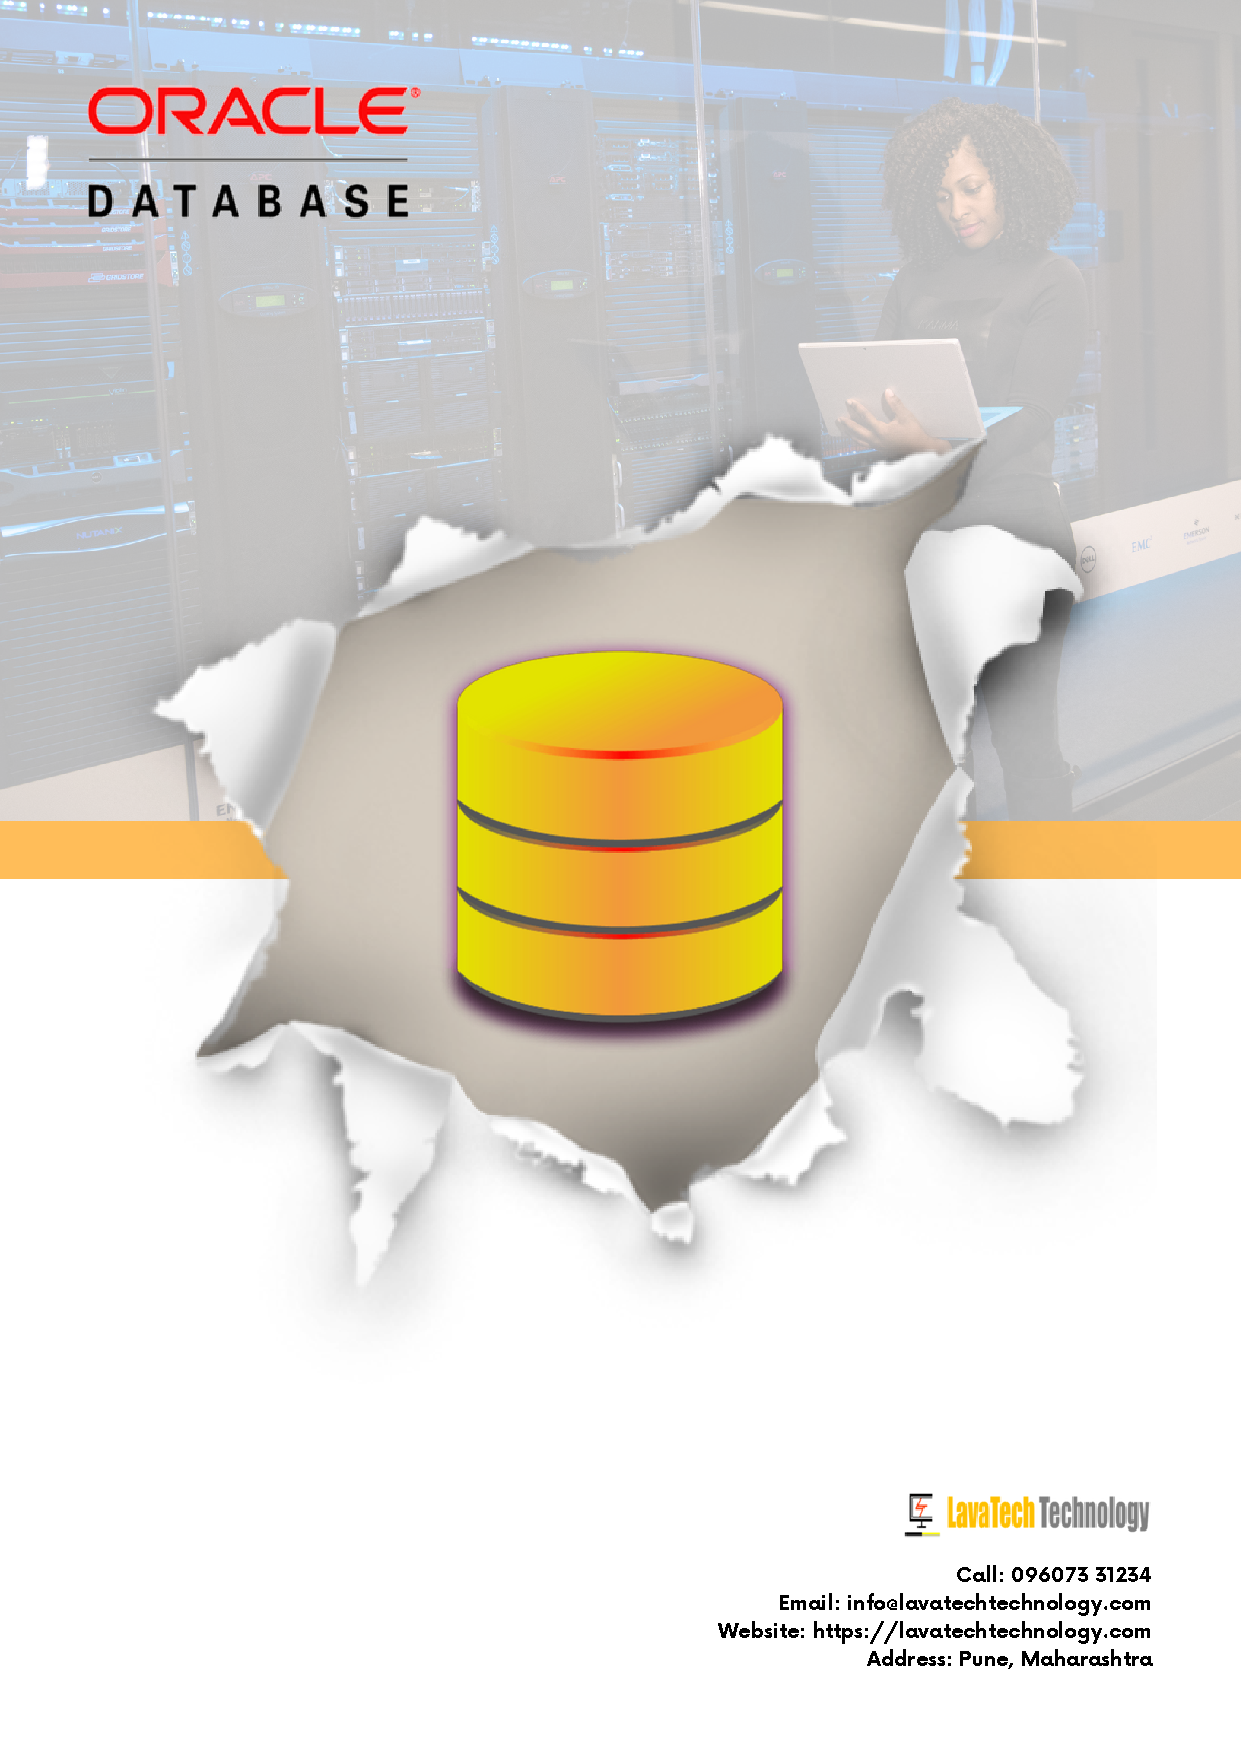
\includegraphics[width=\paperwidth, height=\paperheight]{db.pdf}};
\end{tikzpicture}
\vfill
\endgroup

%----------------------------------------------------------------------------------------
%	COPYRIGHT PAGE
%----------------------------------------------------------------------------------------

\newpage



~\vfill
\thispagestyle{empty}

\noindent Copyright \copyright\ 2024 Lavatech Technology\\ % Copyright notice

The contents of this course and all its modules and related materials, including handouts are
Copyright ©

No part of this publication may be stored in a retrieval system, transmitted or reproduced in any way, including, but not limited to, photocopy, photograph, magnetic, electronic or other record, without the prior written permission of Lavatech Technology.

If you believe Lavatech Technology training materials are being used, copied, or otherwise improperly distributed please e-mail: 
\newline
\textbf{info@lavatechtechnology.com}

\noindent \textsc{Published by Lavatech Technology}\\ % Publisher

\noindent \textit{lavatechtechnology.com}\\ % URL

%\noindent Licensed under the Creative Commons Attribution-NonCommercial 3.0 Unported License (the ``License''). You may not use this file except in compliance with the License. You may obtain a copy of the License at \url{http://creativecommons.org/licenses/by-nc/3.0}. Unless required by applicable law or agreed to in writing, software distributed under the License is distributed on an \textsc{``as is'' basis, without warranties or conditions of any kind}, either express or implied. See the License for the specific language governing permissions and limitations under the License.\\  License information, replace this with your own license (if any)
%
\noindent \textit{January 2024} % Printing/edition date

\afterpage{\blankpage}
\afterpage{\blankpage}


%----------------------------------------------------------------------------------------
%	TABLE OF CONTENTS
%----------------------------------------------------------------------------------------


\usechapterimagetrue % If you don't want to include a chapter image, use this to toggle images off - it can be enabled later with \usechapterimagetrue

\chapterimage{image1.png} % Table of contents heading image

\pagestyle{empty} % Disable headers and footers for the following pages


\tableofcontents



\cleardoublepage % Forces the first chapter to start on an odd page so it's on the right side of the book

\pagestyle{fancy} % Enable headers and footers again

%----------------------------------------------------------------------------------------
%	PART One
%----------------------------------------------------------------------------------------

%\part{System Admin Level I}

%----------------------------------------------------------------------------------------
%	CHAPTER 0
%----------------------------------------------------------------------------------------
%\begin{flushleft}

\begin{figure}[h!]
	\centering
	\includegraphics[scale=.35]{content/chapter1/images/career.png}
\end{figure}

\newpage
\paragraph{Linux Job Titles}
\bigskip
\bigskip
When you're looking for Linux jobs you can earn different job titles. Here are a few to watch out for:
\begin{itemize}
	\item Linux Administrator
	\item Linux System Administrator
	\item Linux System Engineer
	\item Linux Engineer
	\item Operations Engineer
	\item SRE (Site Reliability Engineer)
	\item DevOps Engineer
	\item Platform Engineer
	\item Sysadmin
	\item Release Engineer
	\item Build Engineer
	\item Security Administrator
\end{itemize}

There will be even more variations to the job titles when you add prefixes such as "Junior", "Senior" or "Associate" to the mix.

\end{flushleft}


\newpage

\chapterimage{oracle.png}
\chapter{Oracle RDBMS}
\subsection{Data, database \& DBMS}

\setlength{\columnsep}{3pt}
\begin{flushleft}

	\textbf{Data}
	\begin{itemize}
		\item Data is collection of information that can be recorded \& have meaning.
	\end{itemize}
	
	\textbf{Database}
	\begin{itemize}
		\item Database is collection of interrelated data stored in tables.
		\newimage{0.65}{content/chapter1/images/1.jpg}
	\end{itemize}

	\newpage
	\textbf{DBMS}
	\begin{itemize}
		\item DBMS stands for database management system.
		\item DBMS is software that enables user to create and maintain a database. 
		\item DBMS allows to define, construct and manipulate the database.
		\item Advantages of DBMS:
		\begin{itemize}
			\item Data Independence
			\item Efficient Data Access
			\item Data Integrity and security
			\item Data administration
			\item Concurrent access and Crash recovery
		\end{itemize}
	\end{itemize}
	
\end{flushleft}






%\subsection{Database users}
%
\begin{flushleft}

	\textbf{Database Administrators (DBA):}
	\begin{itemize}
			\item DBA authorizes access to database.
			\item DBA is responsible for:
			\begin{itemize}
				\item Design the database schemas
				\item Security and Authorization
				\item Recovery from failures
				\item Database Tuning
			\end{itemize}
	\end{itemize}
		
	\textbf{Application Programmers:}
	\begin{itemize}
		\item Includes software engineers, software tester etc.
		\item These people can test, debug, document and maintain the database transactions.
	\end{itemize}

	\textbf{End Users:}
	\begin{itemize}
		\item People who require access to database for querying, updating and generating reports like:
		\begin{itemize}
			\item \textbf{Casual end users}:  Require occasional access the database.
			\item \textbf{Sophisticated users}: Business analyst, Managers etc.
		\end{itemize}
		
	\end{itemize}
		
\end{flushleft}

\newpage


\subsection{What is RDBMS?}
\begin{flushleft}
	
	\begin{itemize}
		\item RDBMS is a type of DBMS that stores and manages data in tables. 
		\item It is designed using relational model.
	\end{itemize}

	\textbf{Relational Model}: It is a framework introduced by E.F. Codd in 1970. It organize and manage data within DBMS as follows:
	\begin{itemize}
		\item \textbf{Tables:} 
		\begin{itemize}
			\item Tables are relations.
			\item Table contains rows (records) and columns (attributes or fields).
			\item Each row is unique record.
			\item Each column is attribute.
		\end{itemize}
		
		\item \textbf{Tables have a Primary Key:}
		\begin{itemize}
			\item A primary key is a column (or set of columns) that uniquely identifies each table record. 
			\item Primary key ensures records are not duplicate.
		\end{itemize}
	
		\item \textbf{Foreign Key:}
		\begin{itemize}
			\item Table relations are established using foreign keys. 
			\item A foreign key in one table refers to the primary key in another table.
		\end{itemize}
	
		\item \textbf{Data Integrity:}
		\begin{itemize}
			\item Defines constraints, such as uniqueness, null values, ensures foreign keys reference valid primary keys etc.
		\end{itemize}
	
		\item \textbf{Structured Query Language (SQL):}
		\begin{itemize}
			\item Use SQL (Structured Query Language) for querying and manipulating data. 
			\item SQL allows users to perform operations like SELECT, INSERT, UPDATE, DELETE etc.
		\end{itemize}
	
		\item \textbf{Data Independence:}
		\begin{itemize}
			\item The relational model promotes a separation between physical storage and logical representation of data. 
			\item Changes to the physical storage do not affect data being accessed or queried.
		\end{itemize}
	
		\item \textbf{Normalization:}
		\begin{itemize}
			\item Organize the database tables to minimize redundancy and anomalies.
		\end{itemize}
	
		\item \textbf{Adherence to Codd's Rules:}
		\begin{itemize}
			\item Codd formulated 12 rules  that makes a system fully compliant with relational model.
		\end{itemize}
	
		\item \textbf{ACID Transactions}: RDBMS supports ACID (Atomicity, Consistency, Isolation, Durability) properties.
	\end{itemize}
	
\end{flushleft}

%\subsection{RDBMS features}
%\begin{flushleft}
	
	\begin{itemize}
		\item \textbf{Data Integrity}: RDBMS defines constraints like unique values, data types, table relationships etc. to maintain accurate data.
		
		
		
		\item \textbf{Structured Query Language (SQL)}: RDBMS uses SQL for data query and manipulation.
		
		\item \textbf{Normalization}: RDBMS uses normalization to minimize data redundancy.
		
		\item \textbf{Scalability}: RDBMSs can handle small \& large amounts of data.
		
		\item \textbf{Data Security}: RDBMSs allows administrators to grant different levels of permissions to users and roles.
		
		\item \textbf{Data Backup and Recovery}: RDBMSs provide tools for data backup and recovery.
		
	\end{itemize}

\end{flushleft}

\newpage
%\subsection{Brief on E.F CODD}
%
\begin{flushleft}
	
	Edgar F. Codd formulated a set of 12 rules that define a true RDBMS:
	\begin{itemize}
		\item \textbf{Use table}: 
		\begin{itemize}
			\item Data should be in tables with rows and columns.
		\end{itemize}
		
		\item \textbf{Guaranteed Access Rule}: 
		\begin{itemize}
			\item Data needs to be accessible through table name, primary key value, and column name.
		\end{itemize}
		
		\item \textbf{Systematic Treatment of Null Values}:
		\begin{itemize}
			\item The DBMS must allow field to be null, \& operations can be performed null values.
		\end{itemize} 
	
		\item \textbf{Dynamic Online Catalog Based on the Relational Model}: 
		\begin{itemize}
			\item The database's structure (metadata) must be stored in the same relational format as regular data, accessible to authorized users.
		\end{itemize}
		
		\item \textbf{Comprehensive Data Sublanguage Rule:}
		\begin{itemize}
			\item DBMS must support a comprehensive DML for defining, querying, and manipulating data.
		\end{itemize} 
	
		\item \textbf{Updating Rule:} 
		\begin{itemize}
			\item A table that is theoretically updatable should also be updatable by the system.
		\end{itemize}
		
		\item \textbf{High-Level Insert, Update \& Delete:} 
		\begin{itemize}
			\item The DBMS must support  insert, update, and delete operations without dealing with low-level record management.
		\end{itemize}
		
		\item \textbf{Physical Data Independence:} 
		\begin{itemize}
			\item Changes to the physical storage should not affect the user's ability to access data.
		\end{itemize}
		
		\item \textbf{Logical Data Independence:} 
		\begin{itemize}
			\item Changes to the logical structure (table definitions, relationships) should not affect ability to access the data.
		\end{itemize}
		
		\item \textbf{Integrity Independence:} 
		\begin{itemize}
			\item Integrity constraints ( data uniqueness, datatype etc), must be defined independently of application.
		\end{itemize}
		
		
		\item \textbf{Distribution Independence:}
		\begin{itemize}
			\item Distribution of database over network without impacting the schema.
		\end{itemize} 
	
		\item \textbf{Nonsubversion Rule:} 
		\begin{itemize}
			\item DBMS with low-level language (such as assembly language), should not be able to bypass integrity constraints defined by the high-level language (SQL).
		\end{itemize}
		
	\end{itemize}

\end{flushleft}



\subsection{RDBMS v/s DBMS}
\setlength{\columnsep}{20pt}
\begin{flushleft}

	\tabletwo{
		\textbf{RDBMS} & \textbf{DBMS}	\\
		\hline
		An RDBMS is type of DBMS based on E.F. Codd's relational model &
		DBMSs supports relational model,  hierarchical model , network model, object-oriented model, and key-value.
		\\
		\hline
		RDBMS stores data in tables \& use SQL for querying data. &  
		DBMS stores data using indexing, hashing, or even simple file systems. \\
		\hline
		Eg: RDBMSs include MySQL, PostgreSQL, Oracle Database, Microsoft SQL Server, and SQLite. & 
		Eg: All RDBMSs are DBMSs, DBMS also includes NoSQL like MongoDB and Cassandra. \\
	}
	
\end{flushleft}
\newpage


\subsection{What is database server?}
\begin{flushleft}

	\begin{itemize}
		\item A database server is a software application to \textbf{manage and provide access to DBMS}. 
		\item It is a central repository for DBMS that clients can interact.
		\item Below are some database servers:
		\tablethree{
			\textbf{Company} & \textbf{Database Server} & \textbf{Language} &  \\
			\hline
			Oracle & Oracle Database server & SQL, PL/SQL \\
			\hline
			Microsoft & Microsoft SQL Server & SQL, T-SQL \\
			\hline
			IBM & DB2 & SQL, PL/SQL \\
			\hline
			SUN(acquired by Oracle) & MySQL & SQL, PL/SQL \\
			\hline
			Sybase(acquired by SAP) &
			\begin{itemize}
				\item Sybase
				\item MongoDB
				\item MS Access
				\item FoxPro
			\end{itemize}
			& SQL, TSQL \\
			\hline
			IBM & 
			\begin{itemize}
				\item MainFrame
				\item TeraData
				\item BigData
				\item NoSQL
			\end{itemize}		
			& 
			\begin{itemize}
				\item SQL
				\item SQL
				\item SQL
				\item SQL
			\end{itemize} 
		}
		
	\end{itemize}	
	
	\textbf{What is a Database server used for?}
	\begin{itemize}
		\item Provide 24X7 access to data.
		\item Deal with large amounts of data regularly.
		\item Manage the recovery and security of the DBMS.
		\item Provide remote and concurrent access control.
	\end{itemize}
	
	
	
\end{flushleft}

\newpage
\subsection{RDBMS in Business}
\begin{flushleft}
	
	\newimage{0.64}{content/chapter1/images/2.png}
	
	\textbf{OLTP}
	\begin{itemize}
		\item Stands for \textbf{O}n\textbf{L}ine \textbf{T}ransaction \textbf{P}rocessing.
		\item It is database system to manage and process day-to-day data transactions.
		\item It involve activities characterized by:
		\begin{itemize}
			\item Process transactions quickly.
			\item It involve transaction for insert, update, or delete small amounts of data in database.
			\item Break data into smaller, related tables to avoid data duplication.
			\item Users expect quick responses for applications like e-commerce, banking systems etc.
		\end{itemize}
	\end{itemize}
	
	\bigskip
	\textbf{Data warehouse}
	\begin{itemize}
		\item A data warehouse is a centralized repository for storing large volumes of data from various sources. 
		\item Data once entered into data warehouse cannot be modified.
		\item Data in data warehouse is:
		\begin{itemize}
			\item Consolidated
			\item Historical Data
			\item Non-volatile
		\end{itemize}
		\bigskip
	\end{itemize}

	\textbf{OLAP}
	\begin{itemize}
		\item Stands for \textbf{O}n\textbf{L}ine \textbf{A}nalytical \textbf{P}rocessing
		\item OLAP system are used for:
		\begin{itemize}
			\item Data analysis
			\item Reporting
			\item Facilitate decision-making 
			\item Business intelligence activities
		\end{itemize}
	\end{itemize}

	\textbf{ETL}
	\begin{itemize}
		\item ETL stands for Extract, Transform, Load.
		\item It is iterative process that runs on a scheduled basis to keep the data warehouse updated. 
		\item Data warehousing performs below task:
		\begin{itemize}
			\item Collect data from various sources
			\item Transform it into a suitable format
			\item Load it into data warehouse
		\end{itemize}
	\end{itemize}
	
\end{flushleft}

\newpage
%\subsection{History of Oracle Database}
%\begin{flushleft}
	
	\newimage{0.85}{content/chapter1/images/3.png}
	
\end{flushleft}

\subsection{Oracle Database Installation}
\begin{flushleft}
	

	\begin{itemize}
		\item Install Oracle DB
		\item Install Oracle SQL developer
	\end{itemize}
	
\end{flushleft}

\newpage
\subsection{Oracle DB User}
\begin{flushleft}
	
	\newimage{0.4}{content/chapter1/images/4.png}
	
	Create a local user in Oracle 21c.
	\begin{itemize}
		\item Login as system DBA:
		
		\syntaxblock{
			sqlplus sys/<password>@<TNS service name> as sysdba
		}
		where,
		\begin{itemize}
			\item <password> is the password that you set during oracle installation.
			\item <TNS service name> where Transparent Network Substrate (TNS) operates for connection to Oracle databases.
		\end{itemize}
		\noteblock{
			You can find the current database name using below query:
			\commandblock{
				SELECT ora\_database\_name FROM dual;
			}	
		}
		Eg:
		\commandblock{
		>sqlplus sys/Admin12345@orcl as sysdba
		}
		
		Optionally, you can connect using command prompt with username/password:
		\commandblock{
		> sqlplus / as sysdba
		}
		
		
		\item Once connected to database, alter the session:	
		\commandblock{
		SQL> alter session set "\_oracle\_script"=true;
		}
	
		\item Create a local user using below syntax:
		\syntaxblock{
			SQL> create user <username> identified by <password>; \\
			SQL> grant resource,connect,dba to <username>;
		}
		\item Eg:
		\commandblock{
			SQL> create user jack identified by Admin12345; \\
			SQL> grant resource,connect,dba to jack;
		}
		
		\item Login as local user:
		\syntaxblock{
			sqlplus user/password	
		}
		Eg:
		\commandblock{
			C:$\backslash$Users$\backslash$Admin> \textbf{sqlplus jack/Admin12345}
		}
		
		\newpage
		\item You can check current user using below command:
		\commandblock{
		SQL> \textbf{show user;} \\
		USER is "Jack"
		}
	
		\item You can switch user using below command:
		\commandblock{
			SQL> \textbf{conn jack} \\
			Enter password: \\
			Connected.
		}
	
		\item You can check all user details in "ALL\_USER" table:
		\commandblock{
			SQL> \textbf{select username from ALL\_USER;}
		}
		
		\item You can clear the screen using below command:
		\commandblock{
			SQL> \textbf{cl scr;}
		}
	
		\item You can drop user account using below command:
		\bigskip
		\syntaxblock{
			drop user username; \\
			or \\
			drop user username CASCADE;  
		}
		Eg:
		\commandblock{
			SQL> drop user jack;
		}
	\end{itemize}
	
	\newpage
	
	\textbf{Connecting to Oracle SQL developer}
	
	\begin{itemize}
		\item Start the Oracle SQL developer
		\item Create a new connection by clicking the "+" symbol as shown in screenshot below:

		\newimage{0.4}{content/chapter1/images/image1.png}
		
		\item Enter the connection details as shown and click "Test". 
		\newimage{0.4}{content/chapter1/images/image2.png}
		
		Once the test is successful, select "Connect".
		
		\item Enlarge the "NewConnection" dropdown and notice all the tables are displayed:
		\newpage
		\newimage{0.4}{content/chapter1/images/image3.png}
		
		\item Create a new table by executing below query in worksheet. Click the green run logo on top of worksheet to execute the query.

		\commandblock{
			create table employee(no int, name varchar2(20));
		}
		
		\item Refresh the table to see new table entry:
		\newimage{0.4}{content/chapter1/images/image4.png}
		
		\item Optionally you can execute below query to display all tables:
		\commandblock{
			select * from tab;
		}
		
		
		
	\end{itemize}
	
\end{flushleft}

\newpage
\subsection{What is SQL?}
\begin{flushleft}
	
	\begin{itemize}
		\item SQL stands for \textbf{Structured Query Language}
		\item Pronounced as S.Q.L/Sequel.
		\item This language is used to communicate with Database.
		\item SQL require environment (like SQL *Plus) to implement it's statements
		\item \textbf{SQL is non-procedural language} (means contains only statement and no procedure).
		\item It is case-insensitive language.
		\item SQL is ANSI(American National Standards Institute) standards.
	\end{itemize}
	
\end{flushleft}



%\begin{flushleft}

\begin{figure}[h!]
	\centering
	\includegraphics[scale=.35]{content/chapter1/images/career.png}
\end{figure}

\newpage
\paragraph{Linux Job Titles}
\bigskip
\bigskip
When you're looking for Linux jobs you can earn different job titles. Here are a few to watch out for:
\begin{itemize}
	\item Linux Administrator
	\item Linux System Administrator
	\item Linux System Engineer
	\item Linux Engineer
	\item Operations Engineer
	\item SRE (Site Reliability Engineer)
	\item DevOps Engineer
	\item Platform Engineer
	\item Sysadmin
	\item Release Engineer
	\item Build Engineer
	\item Security Administrator
\end{itemize}

There will be even more variations to the job titles when you add prefixes such as "Junior", "Senior" or "Associate" to the mix.

\end{flushleft}


\newpage

\chapterimage{index3.png}
\chapter{ERD}
\section{ERD}
\subsection{Entity Relationship Diagram (ERD)}
\begin{flushleft}
	
	\begin{itemize}
		\item An ERD is a visual representation of the data model depicting entities and their relationship with each other.
		
		\item ERD components:
		
		\begin{itemize}
			\item \textbf{Entities}: 
			\begin{itemize}
				\item Entities represents real world object having some data.
				\item Eg: Customer, Employee
			\end{itemize}
			
			
			\item \textbf{Attributes}: 
			\begin{itemize}
				\item Attributes are characteristics of entities.
				\item Eg: name, age, phone-number
			\end{itemize}
			
			
			\item \textbf{Relationships}: 
			\begin{itemize}
				\item Relationships define how entities are connected to each other.
				\item Eg: Child and Parent have filiation relationship
			\end{itemize}
			
			\newpage
			\newimage{0.45}{content/chapter1/images/eg1.png}
			
			
			\item \textbf{Cardinality}: 
			\begin{itemize}
				\item Cardinality specify how many instances of one entity are associated with instances of another entity in a relationship. 
				\item 3 types of cardinalities:
				\newimage{0.55}{content/chapter1/images/test100.png}
			\end{itemize}
			
			\newpage
			\item \textbf{Primary Key}: 
			\begin{itemize}
				\item A primary key is an attribute that uniquely identifies an entity. 
				\item It ensures that there are no duplicate records.
			\end{itemize}
			
			
			\item \textbf{Foreign Key}: 
			\begin{itemize}
				\item A foreign key is an attribute in one entity that refers to the primary key of another entity. 
				\item It establishes a link between the two entities.
			\end{itemize}
			
			\bigskip
			\newimage{0.75}{content/chapter1/images/test200.png}
			
			\newpage
			\item \textbf{Diagram Symbols}: Peter Chen invented Chen ERD notation. Symbols used to represent ERD are:
			\bigskip
			\begin{itemize}
				\item \textbf{Entity:}
				\newimage{0.4}{content/chapter1/images/1.png}
				\item \textbf{Attribute:}
				\newimage{0.4}{content/chapter1/images/5.png}
				\item \textbf{Multi-valued attribute:} An attribute can have more than one value. 
				\newimage{0.4}{content/chapter1/images/8.png}
				\newline
				Eg: A student can have more than one phone number.
				\newimage{0.5}{content/chapter1/images/10.png}
				\item \textbf{Derived Attribute:} An attribute that can be derived from other attribute is known as a derived attribute. 
				\newimage{0.6}{content/chapter1/images/11.png}
				\newline
				Eg:  A person's age can be derived from Date of birth.
				\newimage{0.5}{content/chapter1/images/12.png}
				\newpage
				\item \textbf{Primary Key attribute:}
				\newimage{0.4}{content/chapter1/images/6.png}
				\newline
				Eg: Id is unqiue for every student
				\newimage{0.55}{content/chapter1/images/13.png}
				\newpage
				\item \textbf{Relationship:}
				\newimage{0.4}{content/chapter1/images/7.png}			
				\item \textbf{Cardinality:}
				\newimage{0.4}{content/chapter1/images/new.png}
			\end{itemize}
		\end{itemize}
	\end{itemize}
	
	
		
	
	
\end{flushleft}

\newpage
\subsection{Relationship types}
\begin{flushleft}
	
	\begin{itemize}
		\item \textbf{One to One (1:1)}
		\begin{itemize}
			\item Each record in one entity (table) is associated with exactly one record in another entity, and vice versa. 
			\item Eg: Person and Passport is 1:1 relationship
		\end{itemize}
		\bigskip
		\textbf{Person table}
		\bigskip
		\tabletwo{
			\textbf{Fields} & \textbf{Type} \\
			\hline
			person\_id & Primary Key \\
			\hline
			name & \\
			\hline
			date\_of\_birth & \\
			\hline
		}
		\textbf{Passport table}
		\tabletwo{
			\textbf{Fields} & \textbf{Type} \\
			\hline
			passport\_id & Primary Key \\
			\hline
			passport\_number & \\
			\hline
			expiration\_date & \\
			\hline
			person\_id & Foreign Key from Person table \\
			\hline			
		}
		
		\item \textbf{One to Many (1:M)}
		
		\begin{itemize}
			\item A single record in one entity (table) can be associated with multiple records in another entity.
			\item Eg: One manager manages multiple employees
		\end{itemize}
	
		\textbf{Manager table}
		\bigskip
		\tabletwo{
			\textbf{Fields} & \textbf{Type} \\
			\hline
			id & Primary key \\
			\hline
			name & \\
			\hline
			department & \\
			\hline
		}
	
		\newpage
		
		\textbf{Employee table}
		\tabletwo{
			\textbf{Fields} & \textbf{Type} \\
			\hline
			id & Primary key \\
			\hline
			name & \\
			\hline
			department & \\
			\hline
			manager\_id & Foreign key \\
			\hline
		}
	
		\item \textbf{Many to Many (M:M)}
		\begin{itemize}
			\item Each record in one entity can be related to multiple records in the second entity, and vice versa.
			\item An intermediary table ( or junction table) contains foreign keys from both entities involved in the relationship, creating a link between them. 
			\item Eg: One student can enroll for multiple course and 1 course can have multiple students.
		\end{itemize}
	
		\textbf{Students table:}
		\tabletwo{
			\textbf{Fields} & \textbf{Type} \\
			\hline
			student\_id & Primary Key \\
			\hline
			student\_name & \\
			\hline
			date\_of\_birth & \\
			\hline
		}
	
		\textbf{Courses table:}
		\tabletwo{
			\textbf{Fields} & \textbf{Type} \\
			\hline
			course\_id & Primary Key \\
			\hline
			course\_name & \\
			\hline
			instructor & \\
			\hline		
		}
	
		\textbf{Enrollment table (Junction table):}
		\tabletwo{
			\textbf{Fields} & \textbf{Type} \\
			\hline
			enrollment\_id & Primary Key \\
			\hline
			student\_id & Foreign Key \\
			\hline
			course\_id & Foreign Key \\
			\hline
		}
	
	\end{itemize}
	
\end{flushleft}

\newpage
\subsection{ERD example}

\begin{flushleft}


	Example 1: Docter-Patient ERD
	\newimage{0.3}{content/chapter1/images/new5.png}
	
	Example 2: Library system ERD
	\newimage{0.4}{content/chapter1/images/erd.png}

\end{flushleft}

\newpage
%\subsection{Physical data model}
%\begin{flushleft}
	
	\begin{itemize}
		\item Physical data model is detailed data model.
		\item Key components are:
		
		\begin{itemize}
			\item Tables, columns, datatype of columns, primary key \& foreign key. 
			\item Eg:
			
			\newimage{0.5}{content/chapter1/images/new6.png}
			
			\item Relationship cardinality:
			
			\newimage{0.5}{content/chapter1/images/new7.png}
		\end{itemize}
		
	\end{itemize}

\end{flushleft}

\newpage
%\subsection{Physical data model example}
%
\begin{flushleft}
	
	
	Example 1: Student-Course physical data model
	\newimage{0.8}{content/chapter1/images/new9.png}
		
\end{flushleft}

\newpage
%\section{DFD}
%\subsection{Data Flow Diagram (DFD)}
%
\begin{flushleft}
	
	\begin{itemize}
		\item Data flow diagrams (DFD) are used to graphically \textbf{represent data flow}. 		
		\item DFD is divided into:
		\begin{itemize}
			\item \textbf{Logical}: Describes data flow through a system to perform certain functionality. 
			\item \textbf{Physical}: Describes implementation of the logical data flow.
		\end{itemize} 
	\end{itemize}	

	\textbf{DFD Symbols}: 
	\begin{itemize}
		
		\item \textbf{External Entity}
		\begin{itemize}
			\item An external entity is a person, department, etc. that provides data to the system or receives outputs from the system. 
			\item They do not process data.
			\item \textbf{Symbol}:
			\newimage{1}{content/chapter1/images/note3.png}	
		\end{itemize}
		
		\item \textbf{Process}
		\begin{itemize}
			\item A process receives input data and produces output in different form.
			\item Process has a name and function.
			\item Eg: Apply Payment, Calculate Commission, Verify Order
			\item \textbf{Symbol}:
			\newimage{0.5}{content/chapter1/images/note1.png}
		\end{itemize}
		\newpage
		
		\item \textbf{Data Store}
		\begin{itemize}
			\item A data store is a symbol for data storage.
			\item \textbf{Symbol}:
			\newimage{0.7}{content/chapter1/images/note2.png}
		\end{itemize}
		
		\item \textbf{Data Flow}
		\begin{itemize}
			\item A data-flow is a path for data to move from one part of the information system to another. 
			\item \textbf{Symbol}:
			\begin{itemize}
				\item Straight lines with incoming arrows are input data flow
				\item Straight lines with outgoing arrows are output data flows
			\end{itemize}
			\newimage{0.6}{content/chapter1/images/arrow.png}
		\end{itemize}
		
	\end{itemize}
	
	\newpage
	\textbf{Rule of Data Flow}
	
	\begin{itemize}
		\item All flow must begin with and end at a processing step. 
		\newimage{0.7}{content/chapter1/images/arow1.png}
		\item An entity cannot provide data to another entity without processing.
		\newimage{0.7}{content/chapter1/images/note4.png}
		\item Data cannot move directly from an entity to a data story without being processed.
		\newimage{0.7}{content/chapter1/images/note5.png}
		\item Data cannot move directly from a data store without being processed.
		\newimage{0.7}{content/chapter1/images/note6.png}
		
		
	\end{itemize}
	
	\newpage
	
	\textbf{Context-Level Diagram (CLD)}
	\begin{itemize}
		\item A context diagram is the highest level in a data flow diagram.
		\item It contains only one process numbered "\textbf{0.0}" for the entire system. 
		\item CLD split into major processes which give greater detail.
		\item Eg: Library management CLD
		\bigskip
		\newimage{0.55}{content/chapter1/images/CLD.png}
	\end{itemize}
	\newpage
	\textbf{Level 1 DFD}
	\begin{itemize}
		\item CLD can further be exploded to represent details of the processing activities into level 1 DFD.
		\item Each process is numbered as 1.0, 2.0 and so on.
		\item Level 1 DFD is next level of process explosion.
		\item Eg: Level 1 DFD of library management system:
		\bigskip
		\newimage{1.1}{content/chapter1/images/im1.png}
	\end{itemize}

	\newpage
	\textbf{Level 2 DFD}
	\begin{itemize}
		\item A Level 2 DFD provides a more detailed view of a system than a Level 1 DFD. 
		\item The processes identified in the Level 1 DFD are broken down into sub-processes in level 2 DFD.
		\item It provide a more detailed flow at granular level.
		\item Eg: Level 2 DFD of library management system:
		\bigskip
		\newimage{1.1}{content/chapter1/images/im2.png}
	\end{itemize}
	
\end{flushleft}



\chapterimage{index4.png}
\chapter{Datatypes in Oracle DB}
\subsection{Identifiers}
\setlength{\columnsep}{3pt}
\begin{flushleft}

	An identifier refers to a name used to identify database objects such as tables, columns, indexes, views, procedures, and other database elements.
	
	\newline
	Rules for Identifiers:
	\begin{itemize}
		\item Identifiers can consist of \textbf{letters}, \textbf{numbers}, and \textbf{underscore character} (\_).
		\item They must \textbf{start with a letter}.
		\item They can be up to \textbf{30 characters} in length.
		\item Identifiers are \textbf{case-insensitive}. However, you can enclose identifiers in double quotes to make them case-sensitive. For example, "My\_Table" and "my\_table" would be treated as different identifiers.
		\item You \textbf{cannot use reserved words as identifiers} without enclosing them in double quotes.
		\item Common naming conventions is \textbf{camelCase or underscores} to separate words in identifiers (e.g., employee\_id, customerName).
	\end{itemize}


		
\end{flushleft}

\newpage






\subsection{Datatypes}

\begin{flushleft}
	
	\newimage{0.7}{content/chapter3/images/types.png}
	
	\begin{itemize}
		\item \textbf{Character Data Types}
		\begin{itemize}
			\item \textbf{char}: Fixed-length character strings
			\bigskip
			\item For example, if you define a CHAR(10) column and store 'hello' in it, it will occupy 10 bytes of storage, with trailing spaces added to fill the remaining space.

			\item 
			\syntaxblock{
				char(size) \\
				\s where, \\
				\s \textbf{size is optional}
			}
			
			\begin{itemize}	
				\item \textbf{Max size}: 2000 chars/bytes
				\item \textbf{Min size}: 1 char/byte
				\item Eg:
				\commandblock{
					create table sample(grade \textbf{char}, section \textbf{char(3)}); \\
					insert into sample values(\textbf{'C', 'II'}); \\
					select length(section) from sample;
				}
				Notice the length is 3 characters.
			\end{itemize}

			\bigskip
			\item \textbf{nchar}: Store fixed-length unicode character strings.
			\syntaxblock{
				char(size) \\
				\s where, \\
				\s \textbf{size is optional}
			}
			\begin{itemize}
				\item \textbf{Max size}: 2000 char/byte
				\item \textbf{Min size}: 1 char/byte
				\item Eg:
				\commandblock{
					create table sample(name nchar(20)); \\
					insert into sample values('$\alpha$ $\theta$'); \\
					select length(name) from sample;
				}
				Notice the length is 20 characters.
			\end{itemize}

			\noteblock{
				\begin{itemize}
					\item CHAR stores Unicode characters using UTF-16 encoding, but it's not specifically designed for Unicode data. 
					\item NCHAR is explicitly designed for storing Unicode characters. 
				\end{itemize}
			}
			\newpage
			\item \textbf{varchar2}: Variable-length character strings
			\bigskip
			\syntaxblock{
				varchar2(size) \\
				\s where, \\
				\s \textbf{size is not optional}
			}
			\begin{itemize}
				\item \textbf{Max size}: 4000 characters/bytes
				\item Eg:
				\commandblock{
				create table sample(name varchar2(30)); \\
				insert into sample values('Raman'); 
				}
				Notice the length is 5 characters.
			\end{itemize}
			
			\bigskip
			\item \textbf{nvarchar2}: Store variable-length unicode character data.
			\syntaxblock{
				nvarchar2(size) \\
				\s where, \\
				\s \textbf{size is not optional}
			}
			\begin{itemize}
				\item \textbf{Max size}: 4000 char/byte
				\item Eg:
				\commandblock{
					create table sample(name nvarchar2(20)); \\
					insert into sample values('$\alpha$ $\theta$'); 
				}
			\end{itemize}
			
			\noteblock{
				\begin{itemize}
					\item VARCHAR2 uses the database's default character set encoding, which might not support all Unicode characters.
					\item NVARCHAR2 ensuring that it can store characters from any language or script supported by Unicode.
				\end{itemize}
			}
		
			\newpage
			\item \textbf{CLOB}: stands for \textbf{C}haracter \textbf{L}arge \textbf{O}bject
			\bigskip
			\syntaxblock{
				clob
			}
			\begin{itemize}
				\item Store variable-length large character data using the database's character set, which may not or may be Unicode.
				\item \textbf{Max size}: 4 GB
				\item Eg:
				\commandblock{
					create table sample(para clob); \\
					insert into sample values('$\alpha$ $\theta$ data'); 
				}
			\end{itemize}
		
			\bigskip
			\item \textbf{NCLOB}: stands for \textbf{N}ational \textbf{C}haracter \textbf{L}arge \textbf{O}bject
			\bigskip
			\syntaxblock{
				nclob
			}
			\begin{itemize}
				\item Store variable-length large character data in the Unicode character set supporting multilingual text.
				\item \textbf{Max size}: 4 GB
				\item If you need to store different languages, NCLOB is the appropriate choice to ensure compared to CLOB.
				\item Eg:
				\commandblock{
					create table sample(para nclob); \\
					insert into sample values('$\alpha$ $\theta$ data'); 					
				}
			\end{itemize}
					
		\end{itemize}
		
		\item \textbf{Number}
		\begin{itemize}
			\item NUMBER datatype is used to store numeric data, including \textbf{integers} and \textbf{floating-point} numbers.
			\item It is a versatile datatype that can store both fixed-point and floating-point numbers with precision and scale.
			
			\syntaxblock{
				NUMBER(precision, scale)	 \\
				where, \\
				\textbf{Precision (p)}: Specifies the total number of digits that can be stored in the number. This includes both the digits to the left and right of the decimal point. \\
				\textbf{Scale}: Specifies the number of digits to the right of the decimal point. Scale cannot be greater than precision.		
			}
			\item If you don't specify precision and scale, Oracle defaults to NUMBER(38,0), which means it can store numbers with up to 38 digits, all of which can be to the left of the decimal point.
		
			\item Eg:
			
			\begin{itemize}
				\item NUMBER: This defines a numeric column with default precision (38) and scale (0), suitable for storing integers.
				\item NUMBER(10, 2): This defines a numeric column with a precision of 10 and a scale of 2, meaning it can store numbers with up to 10 digits, 2 of which can be to the right of the decimal point.
				\item NUMBER(5): This defines a numeric column with a precision of 5 and a scale of 0, suitable for storing small integers.
			\end{itemize}
			\bigskip
			\noteblock{
				If you add more than 38 digits in Number datatype, Oracle DB can have incorrect behaviour and store incorrect values.
			}
			
		\end{itemize}
		
			\item \textbf{Float}
			\begin{itemize}
				\item FLOAT datatype in Oracle Database is deprecated, and its use is discouraged. 
				\item Instead, Oracle recommends using the NUMBER datatype for precise numeric data and the BINARY\_FLOAT and BINARY\_DOUBLE datatypes for floating-point numbers.
			\end{itemize}
			
			\item \textbf{Binary\_float}
			\begin{itemize}
				\item It stores single-precision 32-bit floating point number. 
				\item Max size: 4 bytes
				\item It provides a precision of approximately 6 to 7 significant decimal digits.
				\syntaxblock{
					float
				}
				\item Eg:
				\commandblock{
					create table sample(no binary\_float); \\
					insert into sample values(122.2);
				}
			\end{itemize}
			
			\item \textbf{Binary\_double}
			\begin{itemize}
				\item It is double-precision 64-bit floating point number. 
				\item Max size: 8 bytes
				\item Double precision provides approximately 15-16 decimal digits of precision.
				\syntaxblock{
					binary\_double
				}
				\item Eg:
				\commandblock{
					create table sample(no binary\_double); \\
					insert into sample values(122.2);
				}
			\end{itemize}		
					
		\end{itemize}
		
		
		\newpage
		\item \textbf{Date \& Time}
		
		\begin{itemize}
			\item \textbf{Date Datatype}		
			\begin{itemize}
				\item Default date format is \textbf{DD-MON-YYYY}
				\item Complete date format is \textbf{DD-MON-YY HH:MI:SS AM} where,
				\begin{itemize}
					\item \textbf{DD}: Day of month
					\item \textbf{MON}: Month name (e.g: "JAN" for January)
					\item \textbf{YY}: Last two digits of year (e.g: "21" for 2021)
					\item \textbf{HH}: Hour in 12-hour format
					\item \textbf{MI}: Minutes
					\item \textbf{SS}: Seconds
					\item \textbf{AM}: Time period, either "AM" or "PM"
				\end{itemize}
				Eg: 26-SEP-23 03:30:00 PM
				
				\item Storage size is 7 bytes.
				\item After Oracle 9i, the allowed range is between \textbf{01-Jan-4712 BC - 31-Dec-9999}
				
				\item Eg:
				\commandblock{
					create table sample(joining\_date date); \\
					insert into sample values('04-Mar-1880'); \\
					insert into sample values('04-Mar-21'); \\
					insert into sample values('4-Mar-98'); 
				}
				\item Date functions:
				\begin{itemize}
					\item \textbf{sysdate}: Returns the current date \& time.
					\newline
					Eg:
					\commandblock{
						select sysdate from dual; \\
						insert into sample values(sysdate);
					}
					\item \textbf{to\_date}: Converts a character to DATE value using a specified format.
					\newline
					Eg:
					\commandblock{
						insert into sample values(to\_date('05-Dec-2022 06:34:23 PM', 'DD-MON-YYYY HH:MI:SS PM'));
					}
					\bigskip
					%\item \textbf{to\_char}: Converts DATE to a character with a specified format.
					%\newline
					%Eg:
					%\commandblock{
					%	select to\_char(joining\_date, 'YYYY-MM-DD HH24:MI:SS') from sample;
					%}
					%\bigskip
					%\item \textbf{add\_months}: Adds specified number of months to a DATE value.
					%\newline
					%Eg:
					%\commandblock{
					%	insert into sample values(add\_months(sysdate,3));
					%}
					%\bigskip
					\item \textbf{extract}: Extracts a date component (e.g., year, month, day) from a DATE value.
					\newline
					Eg:
					\commandblock{
						select extract(year from joining\_date), extract(month from joining\_date), extract(day from joining\_date) from sample; 
					}
					
					%\newpage
					
					%\item \textbf{last\_day}: Return last day of month for given DATE.
					%\commandblock{
					%	select last\_day(joining\_date) from sample;
					%}
					
				\end{itemize}
				
			\end{itemize}
			
			\newpage
			
			\item \textbf{Timestamp}
			\begin{itemize}
				\item Introduced in oracle 9i.
				\item Allows date and time.
				\syntaxblock{
					timestamp(p) \\
					timestamp(p) with timezone \\
					timestamp(p) with local timezone \\
					where, \\
					p stands for precision (optional)
				}
				\bigskip
				\item \textbf{TIMESTAMP(p):} This syntax defines a TIMESTAMP data type with optional precision 'p', specifying the number of digits in the fractional seconds part. If 'p' is not specified, the default precision is 6.
				\codeblock{
					CREATE TABLE sample ( \\
					\s t1 TIMESTAMP(3) \\
					); \\
					\\
					insert into sample values('01-Jan-12 10:34:56.123'); \\
					\\
					insert into sample values('01-Jan-12 10:34:56.123990'); \\
					\\
					select * from sample;
				}
				In this example, the precision is of 3 fractional seconds. Hence, even if you enter more than 3 fractional seconds, it would display only 3 fractional seconds. Adding "AM/PM" is optional.
				\bigskip
				\item \textbf{TIMESTAMP(p) WITH TIME ZONE:} This syntax defines a TIMESTAMP data type with time zone information. It stores date and time information along with the time zone offset from UTC (+00:00).
				\commandblock{
					CREATE TABLE sample ( \\
					\s t1 TIMESTAMP with time zone \\
					); \\
					\\
					insert into sample values('01-Jan-12 10:34:56.123457'); \\
					\\
					insert into sample values('01-Jan-12 10:34:56.123457 AM ASIA/TOKYO'); \\
					\\
					insert into sample values('01-Jan-12 10:34:56.123457 AM +00:00'); \\
					select * from sample;
				}
				In this example, if no timezone is provided, it takes "AM ASIA/CALCUTTA" for first record.
				\bigskip
				\item \textbf{TIMESTAMP(p) WITH LOCAL TIME ZONE}: This syntax defines a TIMESTAMP data type with local time zone handling. It automatically converts the time zone to the session time zone when storing and retrieving data. If  "AM/PM" is not added, it by default takes "AM".
				\newpage
				\commandblock{
					CREATE TABLE sample ( \\
					\s t1 TIMESTAMP with local time zone \\
					); \\
					\\
					insert into sample values('01-Jan-12 10:34:56.123457 AM'); \\
					\\
					insert into sample values('01-Jan-12 10:34:56.123457 AM'); \\
					\\
					insert into sample values('01-Jan-12 10:34:56.123457 AM ASIA/TOKYO'); <- Error \\
					\\
					insert into sample values('01-Jan-12 10:34:56.123457 AM +00:00'); <-- Error\\
					select * from sample;
				}
			
				Difference between normal "TIMESTAMP" and "TIMESTAMP WITH LOCAL TIME ZONE" is that the later, when you retrieve the value, it will be converted to the local time zone of the client application.
				
			
				\noteblock{
					\begin{itemize}
						\item UTC stands for Coordinated Universal Time. 
						\item It is the primary time standard by which the world regulates clocks and time. 
						\item UTC does not change with the seasons like local time zones do, and it is not affected by daylight saving time changes.
					\end{itemize}
				}	
			\end{itemize}
		
			\newpage
			\item \textbf{Interval Year}
			\begin{itemize}
				\item Allows time period in terms of years and months
				\syntaxblock{
					internal year(yp) to month(p) \\
					where, \\
					YP is year precision \\
					p is month precision
				}
				\item Default year precision is 2
				\item Display format: \textbf{YY-MM}
				
				\newimage{0.5}{content/chapter2/images/year.png}
				
				\item Eg:
				\commandblock{
					create table sample(t1 interval year to month); \\
					insert into sample values(interval '3' Year); \\
					insert into sample values(interval '3' month); \\
					insert into sample values('3-4'); \\
					insert into sample values('3-0'); \\
					insert into sample values('0-4');
				}
			\end{itemize}
		
			\bigskip
			\item \textbf{Interval Day}
			\begin{itemize}
				\item Allows time period is terms of days, hours, minutes, seconds and fraction
				\bigskip
				\syntaxblock{
					interval day(dp) to second(p) \\
					where, \\
					dp stands for day precision \\
					p is fractional part of seconds
				}
				\item Default day precision is 2 and default p is 6
				\item Display format: DD HH:MI:SS:FF
				
				\newimage{0.5}{content/chapter2/images/day.png}				
				
				\item Eg:
				\commandblock{
					create table sample(t1 interval day to second); \\
					insert into sample values(INTERVAL '3 04:30:15' DAY TO SECOND); \\
					insert into sample values(Interval '3' hour); \\
					insert into sample values(Interval '3' minute); 
				}
			\end{itemize}
		\end{itemize}
		
		\item \textbf{Binary datatype}:
		\begin{itemize}
			\item \textbf{Raw}: 
			\begin{itemize}
				\item Store fixed-length binary \& hexadecimal (starting Oracle 9i) data.
				\item Eg: encryption keys or binary-encoded data.
				\item \textbf{Dataset} for raw datatype:
				\begin{itemize}
					\item Binary data can be 0 or 1
					\item Hex data is not case-sensitive and can be 0-9 or a-f
					\item Both data must be enclosed in ''
					\item Max size: 2000 bytes
					\item Each character take ½ byte of storage space.
				\end{itemize}
				\bigskip
				\syntaxblock{
					raw(size) \\
					where, \textbf{size is not optional}
				}
				\item Eg:
				\commandblock{
					create table sample(data raw(20));  \\
					insert into sample values('10101011'); \\
					insert into sample values('aaff11');
				}
				
			\end{itemize}

			\item \textbf{Blob (Binary large object)}:
			\begin{itemize}
				\item Store unstructured binary data, such as images, audio files, video files etc.
				\item Max size: 128 TB
				\bigskip
				\syntaxblock{
					blob
				}

				%\item Eg: Inserting image into table
				%\bigskip
				%\commandblock{
				%	SQL> CREATE TABLE image\_table(id number, image BLOB); \\
				%	SQL> host sqlldr user/password@orcl control=load\_image.ctl \\
				%	SQL> select length(image) from image\_table;
				%}
				%Content of load\_image.ctl file:
				%\bigskip
				%\codeblockfull{load\_image.ctl}{
				%	LOAD DATA INFILE 'images.txt' INTO TABLE image\_table FIELDS TERMINATED BY ',' (id , image\_filename FILLER CHAR(100), image  LOBFILE(image\_filename) TERMINATED BY EOF)	
				%}
				%Content of images.txt file:
				%\bigskip
				%\codeblockfull{images.txt}{
				%	1,foo.jpg	
				%}
			

				\item Eg: Insert blank entry in place of image
				\commandblock{
					CREATE TABLE image\_table(id number, image BLOB); \\
					insert into image\_table values(101, EMPTY\_BLOB());
				}
				\item Eg: Insert image in blob datatype using \textbf{utl\_raw.cast\_to\_raw()}
				\commandblock{
					CREATE TABLE image\_table(id number, image BLOB); \\ 
					insert into image\_table values(101, utl\_raw.cast\_to\_raw('C:$\backslash$Users$\backslash$Admin$\backslash$ Pictures$\backslash$test.png') );  \\
					\\
					select * from image\_table;
				}
			
				Notice the output should show \textbf{blob} or the image in image column.
				
				To display image path itself:
				
				Here's a basic approach using Oracle SQL as an example, assuming the image path is stored as text within the BLOB data:
				
				\commandblock{
				SELECT SUBSTR(TO\_CHAR(image), \\
				 INSTR(TO\_CHAR(image), 'path=') + 1) FROM image\_table;
				}
				
				
			\end{itemize}

			%\bigskip
			%\item \textbf{Long raw (deprecated)}:
			%\begin{itemize}
			%	\item Deprecated data type.
			%	\item Store binary data, such as images, audio files, and other binary objects. 
			%	\item Use blob instead of long raw.
			%	\item Max size: 2GB
			%\end{itemize}
		
			\newpage
			
			\item \textbf{Bfile (binary file locator)}:
			\begin{itemize}
				\item Store references to binary files stored in filesystem outside the database.
				\item Data will be stored outside the database.
				\item It is read-only by default. 
				\bigskip
				\syntaxblock{
					bfile
				}

				\item Using bfile:
				\begin{itemize}
					\item Create a directory variable using below query:
					\bigskip
					\syntaxblock{
						create or replace directory <var> as <path>; \\
					}
					As admin user, execute below query:
					\bigskip
					\syntaxblock{
						grant read,write on directory <var> to <user>;	
					}
					\item To access the data stored in a BFILE column, you use the BFILENAME function:
					\bigskip
					\syntaxblock{
						create table xyz(fname \textbf{bfile}); \\ 
						insert into xyz values(\textbf{bfilename('<var>','<filename>')});
					}
				\end{itemize}

				\newpage
				\item Eg: Create a table with bfile field and set a directory path:
				\commandblock{
					create table sample(fname \textbf{bfile}); \\ 
					create or replace directory dir1 as 'C:$\backslash$Users$\backslash$Admin$\backslash$Pictures$\backslash$'); \\ 
					\\
					-- As admin user execute below query \\
					grant read,write on directory dir1 to jack; \\ 
					\\
					insert into sample values(\textbf{bfilename}('dir1','1.png'));
				}
			
			\end{itemize}
		\end{itemize}
		
	
\end{flushleft}

\newpage

\section{Constraints}
\setlength{\columnsep}{3pt}
\begin{flushleft}

	\begin{itemize}
		\item Constraints are rules or conditions enforced on table data.
		\item It maintains data accuracy, integrity and consistency. 
		\item Types of constraints:
		\newimage{1.0}{content/chapter4/images/con.png}

	\end{itemize}
	
	
\end{flushleft}

\newpage


\subsection{Domain Integrity Constraints}
\setlength{\columnsep}{3pt}
\begin{flushleft}
		
	\textbf{default}:
	\begin{itemize}
		\item DEFAULT constraint specify default value for column in table. 
		\item Used when INSERT statement does not provide a value for that column. 

		\syntaxblock{
			CREATE TABLE table\_name ( \\
			\s column1 datatype DEFAULT default\_value, \\
			\s column2 datatype DEFAULT default\_value, \\
			\s -- other columns \\
			);
		}
		Eg: 
		\commandblock{
			CREATE TABLE employees ( \\
			\s employee\_id NUMBER(5), \\
			\s first\_name VARCHAR2(50) DEFAULT 'John', \\
			\s dob date DEFAULT SYSTIMESTAMP, \\
			\s joining\_date date DEFAULT SYSDATE, ); \\
			\\
			insert into employees(employee\_id, first\_name) values (101, 'Ravi'); \\
			\\
			insert into employees(employee\_id, first\_name, dob\_date, joining\_date ) values (101, default, default, default); \\
			\\
			CREATE TABLE employees ( \\
			\s first\_name VARCHAR2(50) DEFAULT 'John', \\
			\s dob date DEFAULT SYSTIMESTAMP, \\
			\s joining\_date date DEFAULT SYSDATE, \\
			); 
		}
		\newpage
		\codecontinue{
			insert into employees(first\_name, dob\_date, joining\_date ) values (default, default, default);
		}
	\end{itemize}


	\textbf{not null}:
	\begin{itemize}
		\item NOT NULL ensures a column cannot contain NULL values. 
		\bigskip
		\noteblock{
			Default has highest priority than Not NULL, so first define default than not null.
		}
		\syntaxblock{
			CREATE TABLE table\_name ( \\
			\s column\_name datatype NOT NULL, \\
			\s -- other columns \\
			); \\
			or \\
			CREATE TABLE table\_name ( \\
			\s column\_name datatype CONSTRAINT constraint\_name NOT NULL, \\
			\s -- other columns \\
			); 
		}
		Eg:
		\commandblock{
			create table student( \\
			\s no number CONSTRAINT c1 not null \\
			); \\
			CREATE TABLE students ( \\
			\s student\_id NUMBER(5) NOT NULL, \\
			\s first\_name VARCHAR2(50) NOT NULL,	\\
			); 	
		}
		\newpage
		\codecontinue{
			create table students( \\
			\s no number DEFAULT 0 NOT NULL,  \\
			); 
		}
	\end{itemize}

	\textbf{check}
	\begin{itemize}
		\item CHECK constraint enforces a condition on column or entire table. 
		\item It ensures data entered into the column meets specific criteria or rules. 
		\item Column level check constraints:
		\bigskip
		\syntaxblock{
			CREATE TABLE table\_name ( \\
			column\_name datatype CONSTRAINT constraint\_name CHECK (condition), \\
			-- other columns \\
			);	 \\
			or \\
			CREATE TABLE table\_name ( \\
			column\_name datatype CHECK (condition), \\
			-- other columns \\
			);	 
		}
		\item Table level check constraints:
		\bigskip
		\syntaxblock{
			CREATE TABLE table\_name ( \\
			column\_name datatype, \\
			CONSTRAINT constraint\_name CHECK (condition) \\
			);	 
		}
		Eg: 
		\commandblock{
			CREATE TABLE orders ( \\
			\s order\_id NUMBER(5), \\
			\s order\_total NUMBER(10, 2) CHECK (order\_total > 0) \\
			);
		}

		\commandblock{
			CREATE TABLE emp( \\
			\s eno number,  \\
			\s CONSTRAINT con1 CHECK(eno IN (1,2,3)) \\
			); \\
			CREATE TABLE emp1( \\
			\s eno number  \\
			\s DEFAULT 10 CHECK(eno in (10,20,30))  \\
			\s NOT NULL \\
			);
		}
		
	\end{itemize}	
\end{flushleft}
\newpage
\subsection{Entity Integrity Constraints}
\setlength{\columnsep}{3pt}
\begin{flushleft}

	\textbf{unique}
	\begin{itemize}
		\item \textbf{Unique} does not allow \textbf{duplicate} values
		\item It allows \textbf{NULL} values (Any number of NULLs)
		\item Can be defined at single or multiple \textbf{columns} or at \textbf{table level}
		\syntaxblock{
			// Column level \\
			CREATE TABLE table\_name ( \\
			\s column1 datatype UNIQUE, \\
			\s column2 datatype CONSTRAINT constraint\_name UNIQUE \\
			);  \\
			// Table level \\
			CREATE TABLE table\_name ( \\
			\s column1 datatype, \\
			\s column2 datatype, \\
			CONSTRAINT constraint\_name UNIQUE(column1, column2,..)\\
			); 
		}
		Eg: Column level
		\commandblock{
			CREATE TABLE product( \\
			\s	id number UNIQUE, \\
			\s	name varchar(50) UNIQUE \\
			); \\
			CREATE TABLE product( \\
			name varchar(50) CONSTRAINT con1 UNIQUE(column\_name) \\
			);
		}
		\newpage
		Eg: Table level
		\commandblock{
			create table product1( \\
			\s no number, \\
			\s constraint constraint\_name unique\_no unique(no) \\
			); \\
			create table product2( \\
			\s no number, \\
			\s name varchar2(20), \\
			\s unique(no,name) \\
			);
		}
	\end{itemize}

	\textbf{Primary key}
	\begin{itemize}
		\item A primary key(PK) constraint can:
		\begin{itemize}
			\item Enforces data uniqueness.
			\item Prevent duplicate or NULL values in column
		\end{itemize}
		\item Other tables can reference the PK column(s) as foreign keys.
		\item PK on multiple columns is called composite primary key.
		\item Oracle database automatically creates a unique index on the primary key column(s). 
		\newimage{0.3}{content/chapter4/images/new.png}
		\syntaxblock{
			// Single column primary key \\
			CREATE TABLE example ( \\
			\s column1 datatype PRIMARY KEY, \\
			\s column2 datatype, \\
			); \\	 
 			// Multiple column primary key \\
			CREATE TABLE example ( \\
			\s column1 datatype, \\
			\s column2 datatype, \\
			\s CONSTRAINT pk\_example PRIMARY KEY(column1, column2...) \\
			);	
		}
		Eg:
		\commandblock{
			create table product( \\
			\s no number primary key, \\
			\s name varchar2(30) \\
			); \\
			CREATE TABLE sample( \\
			\s no number, \\
			\s name varchar2(30), \\
			\s CONSTRAINT pk PRIMARY KEY(no, name) \\
			);
		}
			
	\end{itemize}
 	
\end{flushleft}

\newpage
















\subsection{Referential Integrity Constraints}
\setlength{\columnsep}{3pt}
\begin{flushleft}
	
	\textbf{foreign key}
	\begin{itemize}
		\item A foreign key establishes link between two tables.
		\item It ensures one table's column(foreign key) correspond to another table's primary/unique key(referenced key).
		\item Reference column may be present in same/different table.
		\item It allows:
		\begin{itemize}
			\item Duplicate values
			\item NULL values	
		\end{itemize}
		\item It can be defined on single/multiple column (compsite key).
		\item Can be defined at table level or column level.
		
		\newimage{0.4}{content/chapter4/images/new.png}
	
		\newpage
		\syntaxblock{
			// Table level \\
			CREATE TABLE child\_table ( \\
			\s column1 datatype, \\
			\s column2 datatype, \\
			\s referenced\_column datatype, \\
			\s CONSTRAINT fk\_name FOREIGN KEY \\ 
			\s (referenced\_column) \\ 
			\s REFERENCES parent\_table (primary\_key\_column) \\
			); \\
			// Column level \\
			CREATE TABLE child\_table ( \\
			\s column1 datatype, \\
			\s column2 datatype, \\
			\s referenced\_column datatype CONSTRAINT fk\_name \\
			\s REFERENCES parent\_table(primary\_key\_column) \\
			);
		}
		Eg:
		\commandblock{
			CREATE TABLE product( \\
			\s pno number PRIMARY KEY, \\
			\s pname varchar(20), \\
			); \\
			CREATE TABLE productOrder( \\
			\s no number, \\
			\s pno number CONSTRAINT fk  \\
			\s REFERENCES product(pno) \\
			); 
		}	
		\newpage
		\codecontinue{
			CREATE TABLE productOrder( \\
			\s no number, \\
			\s CONSTRAINT fk FOREIGN KEY(pno)  \\
			\s REFERENCES product(pno) \\
			);
		}
	\end{itemize}
	
	\textbf{ON DELETE SET NULL}
	\begin{itemize}
		\item Specify a foreign key column should be set NULL when corresponding row in parent table is deleted. 
		\bigskip
		\syntaxblock{
			CREATE TABLE child\_table ( \\
			\s column1 datatype, \\
			\s parent\_reference datatype, \\
			\s CONSTRAINT fk\_parent\_reference  \\
			\s FOREIGN KEY (parent\_reference) \\
			\s REFERENCES parent\_table(parent\_id) \\
			\s \textbf{ON DELETE SET NULL} \\
			);
		}
		\item Eg:
		\commandblock{
			CREATE TABLE product( \\
			\s pno number PRIMARY KEY, \\
			\s pname varchar(20) \\
			); 
		}
		\newpage
		\codecontinue{
			create table productOrder( \\
			\s id number, \\
			\s pno number, \\
			\s odate date, \\
			\s constraint fk foreign key(pno)  \\
			\s references product(pno) \\
			\s \textbf{on delete set null} \\
			); \\
			insert into product values(101,'cadbury'); \\
			insert into product values(102,'5-star'); \\
			insert into product values(103,'kitkat'); \\
			insert into productOrder values(201,101,SYSDATE); \\
			insert into productOrder values(202,101,SYSDATE); \\
			insert into productOrder values(203,103,SYSDATE); \\
			insert into productOrder values(204,102,SYSDATE);  \\
			delete from product where pno=101; 
		}
		\bigskip
		\outputblock{
		select * from productOrder; \\
		ID 	\s	PNO \s	ODATE \\
		201	\s  - 	\s	06-OCT-23 \\
		202	\s -  	\s	06-OCT-23 \\
		203 \s	103 \s	06-OCT-23 \\
		204	\s 	102 \s	06-OCT-23 
		}
	\end{itemize}
	
	\newpage
	
	\textbf{ON DELETE CASCADE}
	\begin{itemize}
		\item Specify when a row in the parent table is deleted, all related rows in the child table should be deleted. 
		\bigskip
		\syntaxblock{
			CREATE TABLE child\_table ( \\
			\s column1 datatype, \\
			\s parent\_reference datatype, \\
			\s CONSTRAINT fk\_parent\_reference  \\
			\s FOREIGN KEY (parent\_reference) \\
			\s REFERENCES parent\_table(parent\_id) \\
			\s \textbf{ON DELETE CASCADE} \\
			);
		}
		\item Eg:
		\commandblock{
			CREATE TABLE product( \\
			\s pno number PRIMARY KEY, \\
			\s pname varchar(20) \\
			); \\ 
			create table productOrder( \\
			\s id number, \\
			\s pno number, \\
			\s odate date, \\
			\s constraint fk foreign key(pno)  \\
			\s references product(pno) \\
			\s \textbf{on delete cascade} \\
			); \\
			insert into product values(101,'cadbury'); \\
			insert into product values(102,'5-star'); \\
			insert into product values(103,'kitkat'); \\
			insert into productOrder values(201,101,SYSDATE); 

		}
		\newpage
		\codecontinue{
			insert into productOrder values(202,101,SYSDATE); \\
			insert into productOrder values(203,103,SYSDATE); \\
			insert into productOrder values(204,102,SYSDATE);  \\
			delete from product where pno=101; 
		}	
		\bigskip
		\outputblock{
			select * from productOrder; \\
			ID \s	PNO \s	ODATE \\
			203 \s	103 \s	06-OCT-23 \\
			204 \s	102 \s	06-OCT-23
		}
	\end{itemize}
	
\end{flushleft}



\section{Composite key}
\setlength{\columnsep}{3pt}
\begin{flushleft}
	
	\begin{itemize}
		\item A composite key (or compound key) consists of two or more columns in a table, used together to uniquely identify each row. 
		\item A composite key relies on multiple columns to ensure uniqueness. 
		\item It can be defined only on unique key, primary key  \& foreign key. 
		\item Composite key is possible only at table level.
		\item Eg:
		\commandblock{
			create table product( \\
			\s no number, \\
			\s name varchar2(30), \\
			\s constraint pk primary key (no,name) \\
			);	
		}
	\end{itemize}
	
\end{flushleft}




\chapterimage{index5.png}
\chapter{SQL commands}
\setlength{\columnsep}{3pt}
\begin{flushleft}
	
		SQL commands are used for managing and querying data. SQL commands in Oracle are:
		
		\begin{itemize}
			\item \textbf{DDL} - Data Definition Language
			\item \textbf{DML} - Data Manipulation Language
			\item \textbf{TCL} - Transaction Control Language
			\item \textbf{DCL} - Data Control Language
		\end{itemize}
	
\end{flushleft}

\newpage


\section{Data Definition Language (DDL)}
\setlength{\columnsep}{3pt}
\begin{flushleft}

	\begin{itemize}
		\item DDL command deal with the structure of objects.
		\item DDL interacts with database directly, hence there is implicit commit before \& after statements.
		\newimage{0.5}{content/chapter3/images/success.png}
		\item Due to this, you cannot undo (rollback) the changes done by DDL statement.
		\item As DDL commands interact with database directly, they are faster (performance-wise).
		\item DDL commands:
		\begin{itemize}
			\item create
			\item alter
			\item truncate
			\item rename
			\item drop
			\item flashback
			\item purge
			\item comment
		\end{itemize}
		\item flashback and purge where introduced in Oracle 10g
		\item Let's see each of these in detail.
	\end{itemize}

\end{flushleft}

\newpage




\subsection{CREATE}
\setlength{\columnsep}{3pt}
\begin{flushleft}
	
	\textbf{CREATE} query is used to create:
	\begin{itemize}
		\item \textbf{TABLE}: Table is made up of rows and columns.
	\end{itemize}
	
	Let's see each of these in detail.
	\newline
	\textbf{CREATE TABLE}: Used to create a table
	\begin{itemize}
		\item Create table schema:
		\bigskip
			\syntaxblock{
			CREATE TABLE your\_table\_name ( \\
			\s column1\_name datatype1, \\
			\s column2\_name datatype2, \\
			\s column3\_name datatype3, \\
			\s -- Add more columns as needed \\
			);	
			}
			Eg:
			\bigskip
			\commandblock{
				CREATE TABLE employees ( \\
				\s employee\_id NUMBER(5) PRIMARY KEY, \\
				\s first\_name VARCHAR2(50), \\
				\s last\_name VARCHAR2(50), \\
				\s hire\_date DATE, \\
				\s salary NUMBER(10, 2) \\
				);
			}
		\newpage
		\item Create table using existing tables (with data)
		\bigskip
		\syntaxblock{
			CREATE TABLE your\_table\_name as select column\_name from table\_name;
		}
		Egs:
		\bigskip
		\commandblock{
			create table sample1 as select * from dual; \\
			create table sample2 as select dummy from dual; \\
			create table sample1 as select * from dual where 1 = 1; \\
			create table sample1 as select * from dual where dummy = 'x';		
		}
		\bigskip
		\item Create table using existing tables (only structure)
		\bigskip
		\commandblock{
			create table sample1 as select * from dual where 1 = 2;
		}
	
	\end{itemize}	
	

\end{flushleft}

\subsection{TRUNCATE}

\begin{flushleft}
	\begin{itemize}
		\item TRUNCATE deletes all rows from table.
		\item TRUNCATE does not generate any undo logs, so you cannot roll back the operation.
		\item Truncate does not reclaim space immediately; it releases space to the tablespace, making it available for future inserts. \item Use DROP STORAGE option to immediately release the space.
		\bigskip
		\syntaxblock{
			truncate table table\_name [drop storage];
		}
		\bigskip
		\commandblock{
			truncate table dummy; \\
			truncate table dummy drop storage;
		}
		
	\end{itemize}
	
	
\end{flushleft}

\subsection{RENAME}

\begin{flushleft}
	
	Use RENAME command to rename a table or a column. 
	\begin{itemize}
		\item Renaming a table:
		\bigskip
		\syntaxblock{
			RENAME old\_table\_name TO new\_table\_name;	
		}		
		Eg:
		\commandblock{
			RENAME employees TO staff;
		}
		\bigskip
		\item Renaming a column:
		\bigskip
		\syntaxblock{
			ALTER TABLE table\_name RENAME COLUMN old\_column\_name TO new\_column\_name;
		}
		Eg:
		\commandblock{
			alter table employee rename column name TO first\_name;
		}
		\bigskip
		\item Renaming a constraint:
		\syntaxblock{
			ALTER TABLE table\_name RENAME CONSTRAINT old\_name TO new\_name;
		}
		\newpage
		Eg:
		\commandblock{
			CREATE TABLE products( \\
			\s no number, \\
			\s name varchar2(20), \\
			\s CONSTRAINT p PRIMARY KEY(no) \\
			); \\
			ALTER TABLE products RENAME CONSTRAINT p TO pk;
		}
	\end{itemize}
	
	
\end{flushleft}

\subsection{ALTER}
\setlength{\columnsep}{3pt}
\begin{flushleft}
	
	The ALTER command modify existing tables, indexes, constraints, etc. 
	
	\syntaxblock{
		ALTER TABLE table\_name ADD/MODIFY/DROP/RENAME/SET UNUSED/ENABLE/DISABLE;
	}
	\begin{itemize}
		\item \textbf{Rename column}
		
		\syntaxblock{
			ALTER TABLE table\_name \textbf{RENAME} column old\_column TO new\_column;	
		}

		Eg:
		\commandblock{
			CREATE TABLE product(no NUMBER); \\
			ALTER TABLE product \textbf{RENAME} column no TO id;
		}
	
		\item \textbf{Add single column}
		\bigskip
		\syntaxblock{
			ALTER TABLE table\_name \textbf{ADD} column\_name datatype;	 \\
			or \\
			ALTER TABLE table\_name \textbf{ADD} (column\_name datatype);
		}
		Eg:
		\commandblock{
			CREATE TABLE product(no NUMBER); \\
			ALTER TABLE product \textbf{ADD} name VARCHAR2(30); \\
			or \\
			ALTER TABLE product ADD (name VARCHAR2(30));
		}
		\bigskip
		\outputblock{
			DESC product; \\
			Column \s	Null? \s	Type \\
			NO	\s  - \s 	NUMBER \\
			NAME	\s  - \s	VARCHAR2(30)
		}
		\item \textbf{Add multiple column}
		\bigskip
		\syntaxblock{
			ALTER TABLE table\_name \textbf{ADD}(column1\_name datatype,column2\_name datatype); 
		}

		Eg:
		\commandblock{
			CREATE TABLE product(no NUMBER); \\ 
			ALTER TABLE product ADD(name VARCHAR2(20), grade CHAR(3));
		}
		\bigskip
		\outputblock{
			DESC product; \\
			Column \s	Null? \s	Type \\
			NO \s	 - \s 	NUMBER \\
			NAME	\s - \s 	VARCHAR2(20) \\
			GRADE \s	 - \s 	CHAR(3)
		}
	
		\bigskip
		\item \textbf{Modify single column size}
		\syntaxblock{
			ALTER TABLE table\_name \textbf{MODIFY} column\_name DATATYPE(SIZE);  \\
			or \\
			ALTER TABLE table\_name \textbf{MODIFY}(column\_name DATATYPE(SIZE)); 
		}
		Eg:
		\commandblock{
			CREATE TABLE product(name VARCHAR2(10)); \\
			ALTER TABLE product MODIFY(name VARCHAR2(25)); 
		}
		\bigskip
		\outputblock{
			DESC product; \\
			Column \s	Null? \s	Type   \\
			NAME  \s  -  \s 	VARCHAR2(25)   
		}

		\item \textbf{Modify multiple column size}
		\syntaxblock{
			ALTER TABLE table\_name \textbf{MODIFY}(column1\_name DATATYPE(SIZE), 
			column2\_name DATATYPE(SIZE)); 
		}
		Eg:
		\commandblock{
			CREATE TABLE product(no NUMBER(2), name VARCHAR2(10)); \\
			ALTER TABLE product MODIFY(no NUMBER(3), name VARCHAR2(25)); 
		}
		\bigskip
		\outputblock{
			DESC product; \\
			Column \s 	Null? \s	Type \\
			NO	 \s - \s 	NUMBER(3,0)  \\
			NAME \s	 - \s 	VARCHAR2(25)
		}
		
		\item \textbf{Drop single column}
		\syntaxblock{
			ALTER TABLE table\_name \textbf{DROP} COLUMN column\_name;  \\
			or \\
			ALTER TABLE table\_name \textbf{DROP}(column\_name);
		}
		Eg:
		\commandblock{
			CREATE TABLE product(no NUMBER(2), name VARCHAR2(10)); \\
			ALTER TABLE product DROP COLUMN name;
		}

		\outputblock{
			DESC product; \\
			Column \s	Null? \s	Type \\
			NO	\s -  \s	NUMBER(2,0)
		}
		\item \textbf{Drop multiple column}
		\syntaxblock{
			ALTER TABLE table\_name \textbf{DROP}(column1\_name, column2\_name);
		}
		Eg:
		\commandblock{
			CREATE TABLE product(no NUMBER(2), name VARCHAR2(10), grade CHAR(2)); \\
			ALTER TABLE product DROP(name, grade);
		}
		\bigskip
		\outputblock{
			DESC product; \\
			Column \s	Null? \s	Type \\
			NO \s	 - \s 	NUMBER(2,0)
		}
		\item \textbf{Hide single column}
		\syntaxblock{
			ALTER TABLE product SET UNUSED COLUMN column\_name; \\
			or \\
			ALTER TABLE product SET UNUSED(column\_name);
		}

		Eg:
		\commandblock{
			CREATE TABLE product(no NUMBER(2), name VARCHAR2(10), grade CHAR(2)); \\
			insert into product values(11, 'cadbury','AB'); \\
			insert into product values(12, 'munch','AC'); \\
			alter table product set unused column grade; 
		}
		\bigskip
		\outputblock{
			select * from product; \\
			NO \s	NAME \\
			11 \s	cadbury \\
			12 \s	munch
		}
	
		\item \textbf{Hide multiple column}
		\syntaxblock{
			ALTER TABLE product SET UNUSED(column1\_name, column2\_name);
		}
		Eg:
		\commandblock{
			CREATE TABLE product(no NUMBER(2), name VARCHAR2(10), grade CHAR(2)); \\
			insert into product values(11, 'cadbury','AB'); \\
			insert into product values(12, 'munch','AC'); \\
			alter table product set unused(name,grade); 
		}
		\bigskip
		\outputblock{
			select * from product; \\
			NO \\
			11 \\
			12 
		}

		\quest{Why should we hide the column and not drop it directly?}{
			\begin{itemize}
				\item Dropping column with high volume of data during working hours can consume a lot of time.
				\item Hence, during working hours, we can hide the column instead of dropping it
				\item In non-working hours, we can remove the column.
			\end{itemize}
		}
		\bigskip
		\quest{After hiding a column, can we add a new column with same name?}{
			\begin{itemize}
				\item Yes, as once the column is hidden, we cannot unhide it again. We can only drop the column after hiding it.
				\item Hence we can add a colum with same name.
			\end{itemize}
		}
	
	\end{itemize}

\end{flushleft}


\newpage


\subsection{DROP}

\begin{flushleft}
	
	\begin{itemize}
		\item You can drop (delete) database objects using the DROP statement.
		\item Deleted objects are moved to Recycle Bin.
	\end{itemize}
	
	
	
	\noteblock{
		\begin{itemize}
			\item Until Oracle 9i, dropping an object deletes it permanently.
			\item In Oracle 10g, recycle bin concept was introduced.	
		\end{itemize}
	}

	\textbf{Drop table}
		
	\syntaxblock{
			DROP TALBE table\_name
	}
	Eg:
	\commandblock{
			DROP TABLE product;
	}
		
\end{flushleft}
\newpage
\subsection{FLASHBACK}

\begin{flushleft}

	\begin{itemize}
		
		\item A deleted table is present in recycle bin.
		\item Eg: Checking table in recycle bin
		\outputblock{
			SHOW RECYCLEBIN; \\
			no rows selected
		}
		\bigskip
		\commandblock{
			CREATE TABLE emp(no NUMBER); \\
			INSERT INTO emp VALUES(101); \\
			DROP TABLE emp;
		}
		\bigskip
		\outputblock{
			SHOW RECYCLEBIN; \\
			ORIGINAL NAME \s RECYCLEBIN NAME \s OBJECT TYPE \s DROP TIME \\
			--------------------------------------------------------------\\
			EMP \S BIN9820203/==2930 \s TABLE \s 2023-02-08:13:11:11
		}
		
		\item A Flashback Query allows to retrieve deleted table.
		\bigskip
		\syntaxblock{
			FLASHBACK TABLE table\_name TO BEFORE DROP;
		}
		
		\item Eg:
		\commandblock{
			FLASHBACK TABLE emp TO BEFORE DROP; 
		}
		\newpage
		\outputblock{
			SELECT * FROM emp; \\
			NO \\
			------\\
			101
		}
		
	\end{itemize}
		
		
\end{flushleft}

\subsection{PURGE}

\begin{flushleft}

	\begin{itemize}
		\item Introduced in Oracle 10g, the PURGE statement permanently removes object from the \textbf{Recycle Bin}. 
		\bigskip
		\syntaxblock{
			PURGE TABLE table\_name
		}
		\item Eg:
		\commandblock{
			PURGE TABLE product; 
		}
		Confirm table is deleted from Recycle Bin.
		\bigskip
		\outputblock{
			SHOW RECYCLEBIN;	
		}
		
	\end{itemize}	
	
\end{flushleft}

%\subsection{COMMENT}
%
\begin{flushleft}
	
	\begin{itemize}
		\item Create comments on tables and columns to provide descriptions.
		\item Create comment on table:	
		\bigskip
		\syntaxblock{
			COMMENT ON TABLE table\_name IS 'Table comment';
		}
		\item Eg:
		\commandblock{
			CREATE TABLE product(no NUMBER); \\	
			COMMENT ON TABLE product IS 'Product table'; 
		}
		View comments stored in \textbf{user\_tab\_comments} table:
		\bigskip
		\outputblock{
			SELECT COMMENTS FROM USER\_TAB\_COMMENTS WHERE TABLE\_NAME='PRODUCT'; \\
			COMMENTS \\
			--------------- \\
			Product Details
		}
		\item Create comment on column:
		\bigskip
		\syntaxblock{
			COMMENT ON COLUMN table\_name.column\_name IS 'Your column comment';
		}	
		Eg:
		\commandblock{
			CREATE TABLE product(no NUMBER); \\	
			COMMENT ON COLUMN product.no IS 'Product ID';
		}
		View comments stored in \textbf{user\_col\_comments} table:
		\bigskip
		\outputblock{
			SELECT comments FROM USER\_COL\_COMMENTS WHERE table\_name='PRODUCT'; \\
			COMMENTS \\
			--------------- \\
			Product ID
		}	
	\end{itemize}
	 	
\end{flushleft}
\newpage
\section{Data Manipulation Language (DML)}

\begin{flushleft}
	
	\begin{itemize}
		\item DML commands deal with data only.
		\item DML commands interact with \textbf{buffer first}.
		\item Data will be stored in buffer initially.
		\item On commit, the buffer content will be transferred to database.
		\item You can undo (\textbf{rollback}) the changes before commit.
		\item Due to buffer, the performance is relatively slow.
		\item Row-level locks occur implicitly on the modified rows:
		\begin{itemize}
			\item Write operations in DML places \textbf{implicit row-level lock on rows} being modified for that particular user. 
			\item If 100 rows are deleted/modified, those row will be locked for that user. \item Once record is locked, other users cannot modify the row unless lock owner releases the lock. 
			\item However locked row is readable by other users.
		\end{itemize}
		
		\newimage{0.45}{content/chapter3/images/new1.png}
		
		\item DML commands:
		\begin{itemize}
			\item insert
			\item update
			\item delete
			\item merge
		\end{itemize}
		
	\end{itemize}
	
\end{flushleft}

\newpage
\subsection{INSERT}

\begin{flushleft}
	
	\begin{itemize}
		\item INSERT statement adds one or more rows of data to an already created table.
		\bigskip
		\syntaxblock{
			INSERT INTO table\_name[(col1, col2, col3...)] VALUES(value1, value2, value3,...);
		}		
		Eg:
		\commandblock{
			CREATE TABLE product(id NUMBER, name VARCHAR2(20)); \\
			INSERT INTO PRODUCT(id,name) VALUES(101,'cadbury'); \\
			INSERT INTO PRODUCT VALUES(102,'munch');
		}
		
		\item \textbf{'\&'} is default substitution variable wherein it will ask user to enter the value.
		\bigskip
		\syntaxblock{
			INSERT INTO table\_name VALUES(\&col1, \&col2, \&col3,...);
		}
		Eg:
		\outputblock{
			\textbf{INSERT INTO PRODUCT VALUES(\&no, '\&name');} \\
			Enter value for no: 101 \\
			Enter value for name: cadbury \\
			old 1: insert into product values(\&no, '\&name') \\
			new 1: insert into product values(101, 'cadbury') \\
			1 row created. 
		}
		\newpage
		\outputblock{
			\textbf{INSERT INTO PRODUCT VALUES(\&a, '\&b');} \\
			Enter value for no: 102 \\
			Enter value for name: munch \\
			old 1: insert into product values(\&a, '\&b') \\
			new 1: insert into product values(102, 'munch') \\
			1 row created. 
		}
		
		\item Insert record using records of another table:
		\syntaxblock{
			INSERT INTO table\_name SELECT col1,col2,.. FROM another\_table\_name; 
		}
		Eg:
		\commandblock{
			INSERT INTO product SELECT * FROM items; \\
			INSERT INTO product(id, name) SELECT id,name FROM items; 
		}	
	\end{itemize}
	
\end{flushleft}

\subsection{UPDATE}

\begin{flushleft}
	
	UPDATE statement modifies existing records in a table. 
	
	\syntaxblock{
		Updating all records: \\
		UPDATE table\_name SET col1 = value1, col2 = value2,...; 
		\\
		Updating particular record: \\
		UPDATE table\_name SET col = value WHERE CONDITION; 
	}
	Eg: Update all records
	\commandblock{
		UPDATE emp SET ename = 'test';
	}
	Eg: Update particular records
	\commandblock{
		UPDATE emp SET ename = 'test' WHERE eno = 101;
	}
	
\end{flushleft}

\subsection{DELETE}

\begin{flushleft}
	
	\begin{itemize}
		\item DELETE query remove specific rows from a table:
		\syntaxblock{
			DELETE FROM table\_name WHERE conditions;
		}
		
		\item DELETE query remove all rows from a table:
		\syntaxblock{
			DELETE FROM table\_name;
		}
		Eg:
		\commandblock{
			DELETE FROM product;	 \\
			DELETE FROM product WHERE id=101;
		}
	\end{itemize}	
	
\end{flushleft}

\newpage
\subsection{MERGE}

\begin{flushleft}
	\begin{itemize}

	\item Support insert and update statement in single statement.
	\item Introduced in Oracle 9i.
	\item To insert \& update records:
	\bigskip
	\syntaxblock{
		MERGE INTO target\_table alias1  \\
		\s USING source\_table alias2 \\
		\s ON (condition) \\
  		\s WHEN MATCHED THEN \\
		\s UPDATE SET column1 = value1, column2 = value2, ... \\
		\s WHEN NOT MATCHED THEN \\
		\s INSERT (column1, column2, ...) \\
		\s VALUES (value1, value2, ...);	
	}
	\bigskip
	\noteblock{
		Columns names present in condition statement must not be present in update clause.
	}
	Eg: Consider below table:
	\bigskip
	\commandblock{
		create table product1(no number, name varchar2(20)); \\
		insert into product1 values(101,'Cadbury'); \\
		insert into product1 values(102,'Munch'); \\
		insert into product1 values(103,'Perk');
	}
	Create another empty table:
	\bigskip
	\commandblock{
		create table product2(no number, name varchar2(20));
	}
	\newpage
	Using merge, you can insert/update records from product1 table to product2:
	\bigskip
	\commandblock{
		MERGE INTO product2 p2 \\
		\s USING product1 p1 \\
		\s ON (p1.no = p2.no) \\
		\s WHEN MATCHED THEN \\
		\s UPDATE SET p2.name = p1.name \\
		\s WHEN NOT MATCHED THEN \\
		\s INSERT (no, name) \\
		\s VALUES (p1.no, p1.name);
	}

	\end{itemize}
\end{flushleft}

\section{Data Query Language (DQL)}

\begin{flushleft}
	
	Data Query Language (DQL) is used to fetch the data from database. It uses only one command i.e SELECT.
	
\end{flushleft}

\subsection{SELECT}

\begin{flushleft}
	
	Used to select the attribute based on the condition described by WHERE clause.
	
	\syntaxblock{
		SELECT column1, column2, ... \\
		FROM table\_name; \\
		or \\
		SELECT column1, column2, ... \\
		FROM table\_name \\
		WHERE [condition];
	}
	The [condition] can be any SQL expression, specified using comparison or logical operators like \textbf{>, <, =, <>, >=, <=, LIKE, NOT, IN, BETWEEN} etc.

	Eg:
	\commandblock{
		CREATE TABLE emp(id NUMBER, name VARCHAR2(20)); \\
		INSERT INTO emp VALUES(101, 'Ram'); \\
		INSERT INTO emp VALUES(102, 'Ravi'); \\
		INSERT INTO emp VALUES(103, 'Sham'); 
	}
	\outputblock{
		select id,name   \\
		2  from emp     	\\
		3  where id>102;	\\
		\\
		ID \s NAME		\\
		---------- \s -------------	\\
		103 \s Sham	
	}
	
	\textbf{Variations with select query}:
	
	\begin{itemize}
		\item \textbf{Wildcard character}: \textbf{*} is the wildcard character to select all columns in a table.
		\newline
		Eg:
		\commandblock{
			SELECT * FROM employees;
		}
		\item \textbf{Column Aliases}: 
		\begin{itemize}
			\item Make column names more readable by setting alias for column name.
			\item You can use single quotes ('), double quotes (") and square brackets ([]) to create an alias.
			\newpage
			\item Eg:
			\commandblock{
				SELECT
				FName AS "First Name", \\
				MName AS 'Middle Name', \\
				LName AS [Last Name] \\
				FROM employees;
			}
			\item If the alias has a single word you can write it without quotes or brackets.
			\item Eg:
			\commandblock{
				SELECT \\
				FName AS FirstName, \\
				LName AS LastName \\
				FROM employees;
			}
		\end{itemize}
		\item \textbf{COUNT returns total number of records}:
			\bigskip
			\syntaxblock{
				SELECT Count(*) column\_name  FROM table\_name;
			}
			Eg:
			\codeblock{
				CREATE TABLE corder ( \\
				order\_id NUMBER, \\
				customer\_id NUMBER, \\
				order\_amount NUMBER \\
				); \\
				insert into corder values(101, 201, 3400); \\
				insert into corder values(102, 202, 400); \\
				insert into corder values(103, 201, 100); \\
				insert into corder values(104, 202, 2300);  
			}
			\newpage
			\outputblock{
				SELECT COUNT(*) total  FROM corder; \\
				4
			}
		

		\item \textbf{Selecting with table alias}:
		\bigskip
		\commandblock{
			SELECT e.Fname, e.LName \\
			FROM Employees e
		}
		The Employees table is given the alias 'e' directly after the table name.
		
		\bigskip 
		\item \textbf{Selecting with more than 1 condition}
		\begin{itemize}
			\item \textbf{AND}: Makes sure all condition are true.
			\bigskip
			\commandblock{
				SELECT name FROM persons WHERE gender = 'M' AND age > 20;
			}
			\item \textbf{OR}: Makes sure at least once condition is true.
			\bigskip
			\commandblock{
				SELECT name FROM persons WHERE gender = 'M' OR age < 20;
			}
		
			\item These keywords can be combined to allow for more complex criteria combinations:
			\bigskip
			\commandblock{
				SELECT name \\
				FROM persons \\
				WHERE (gender = 'M' AND age < 20) \\
				OR (gender = 'F' AND age > 20);
			}	
		\end{itemize}
		\item \textbf{Selecting with Aggregate functions}:
		\begin{itemize}
			\item \textbf{AVG()}: Return the average of values selected.
			\bigskip
			\commandblock{
				SELECT AVG(Salary) FROM employees; \\
				SELECT AVG(Salary) FROM employees where DepartmentId = 1;
			}
			\item \textbf{MIN()}: Returns the minimum of values selected.
			\bigskip
			\commandblock{
				SELECT MIN(Salary) FROM employees;
			}
			\item \textbf{MAX()}: Returns the maximum of values selected.
			\bigskip
			\commandblock{
				SELECT MAX(Salary) FROM employees;
			}
			\item \textbf{COUNT()}: Returns the count of values selected.
			\bigskip
			\commandblock{
				SELECT COUNT(*) FROM employees; \\
				SELECT COUNT(*) FROM employees WHERE managerId IS NOT NULL \\
				SELECT COUNT(managerId) FROM employees;
			}

			Count can also be combined with the distinct keyword for a DISTINCT count.
			\bigskip
			\commandblock{
				Select COUNT(DISTINCT DepartmentId) FROM employees;
			}
			\item \textbf{SUM()}: Returns the sum of the values selected for all rows.
			\bigskip
			\commandblock{
				SELECT SUM(Salary) FROM employees;
			}
		\end{itemize}
		
			\item \textbf{Select with condition of multiple values from column}:
			\bigskip
			\commandblock{
				SELECT * FROM Cars WHERE status IN ('Waiting', 'Working') \\
				or \\
				SELECT * FROM Cars WHERE (status = 'Waiting' OR status = 'Working')
			}
			\bigskip
			\noteblock{
				value IN ( <value list> ) is a shorthand for disjunction (logical OR).
			}
			\item \textbf{Selection with sorted results}:
			\bigskip
			\commandblock{
				SELECT * FROM employees ORDER BY name; \\
				SELECT * FROM employees ORDER BY name DESC; \\
				SELECT * FROM employees ORDER BY name ASC; \\
				SELECT * FROM employees ORDER BY lame ASC, name ASC
			}

			To save retyping the column name in the ORDER BY clause, use column's number. Column numbers start from 1.
			\bigskip
			\commandblock{
				SELECT Id, FName, LName, PhoneNumber FROM employees ORDER BY 3
			}
		
			Use ORDER BY with TOP to return the top x rows based on a column's value:
			\bigskip
			\commandblock{
				SELECT TOP 5 DisplayName, Reputation FROM Users ORDER BY Reputation desc
			}
			
			\textbf{Order by Alias}: 
			\bigskip
			\commandblock{
				SELECT DisplayName, JoinDate as jd, Reputation as rep \\
				FROM Users \\
				ORDER BY jd, rep
			}
			
			\textbf{Sorting by multiple columns}:
			\bigskip
			\commandblock{
				SELECT DisplayName, JoinDate, Reputation FROM Users ORDER BY JoinDate, Reputation
			}
			
			
			\item \textbf{Selecting with null}: 
			\bigskip
			\commandblock{
				SELECT Name FROM Customers WHERE PhoneNumber IS NULL
			}
			\bigskip
			\noteblock{
				Selection with nulls take a different syntax. Don't use =, use IS NULL or IS NOT NULL instead.
			}
			\item \textbf{Select distinct (unique values only)}
			\bigskip
			\commandblock{
				SELECT DISTINCT ContinentCode
				FROM Countries;
			}
			\item \textbf{Select rows from multiple tables}:
			\bigskip
			\commandblock{
				SELECT * FROM table1, table2; \\
				SELECT table1.column1, table1.column2, table2.column1  \\
				FROM table1, table2
			}
			\bigskip
			\item \textbf{GROUP BY}
			\begin{itemize}
				\item Results of a SELECT query can be grouped by one or more columns using the GROUP BY statement. 
				\item This generates a table of partial results, instead of one result. 
				\item GROUP BY can be used with aggregation functions using the HAVING statement to define how non-grouped columns are aggregated.
				\item It might be easier if you think of GROUP BY as "for each" for the sake of explanation.

				\item Eg: Consider below table:
				\codecontinue{
					EmpID \s MonthlySalary \\
					1 \s\s 200 			 \\
					1 \s\s 300				 \\
					2 \s\s 300				 
				}
				\bigskip
				\outputblock{
					SELECT EmpID, SUM (MonthlySalary) \\
					FROM Employee \\
					GROUP BY EmpID \\
					------------------------------ \\
					1 \s \s 500 \\
					2 \s \s 300 \\
				}			
			\end{itemize}
			
		
			\item \textbf{Filter GROUP BY results using a HAVING clause}
			\begin{itemize}
				\item A HAVING clause is used in conjunction with the GROUP BY clause to filter the results of a query based on the result of an aggregate function. 
				\item Eg: Consider below table
				\bigskip
				\commandblock{
					CREATE TABLE orders ( \\
					\s order\_id NUMBER, \\
					\s customer\_id NUMBER, \\
					\s order\_amount NUMBER \\
					); \\
					INSERT INTO orders VALUES (1, 101, 500); \\
					INSERT INTO orders VALUES (2, 101, 700); \\
					INSERT INTO orders VALUES (3, 102, 300); \\
					INSERT INTO orders VALUES (4, 103, 900); \\
					INSERT INTO orders VALUES (5, 103, 600);
				}

				Retrieve only those customers who have a total order value greater than 1000:
				\commandblock{
					SELECT customer\_id, SUM(order\_amount) AS total\_order\_value \\
					FROM orders \\
					GROUP BY customer\_id \\
					HAVING SUM(order\_amount) > 1000;
				}
			
			\end{itemize}

	\end{itemize}
\end{flushleft}
\newpage
\subsection{DESCRIBE}

\begin{flushleft}
	
	\textbf{DESCRIBE} or \textbf{desc}
	\begin{itemize}
		
		\item In Oracle Database, the DESCRIBE statement is used to retrieve metadata information about a database object, such as a table, view, or synonym. 
		\item It provides details about the structure of the object, including column names, data types, constraints, and other properties.
		
		
		\syntaxblock{
			describe table\_name; \\
			or \\
			Desc table\_name; \\
			or \\
			desc schema\_name.table\_name; 
		}	
		Mostly, the schema\_name is the user name.	
		Eg:
		
		\commandblock{
			desc jack.emp1;
		}
		
		

	\end{itemize}

\end{flushleft}

\newpage

\section{Data Control Language (DCL)}

\begin{flushleft}
	
	\begin{itemize}
		\item Data Control Language(DCL) command deal with \textbf{privileges} only \& deal with database directly.
		\item DCL command enforces an implicit commit before and after statement because of direct commit, hence rollback is not possible.
		\item Performance is faster due to direct interaction with database.
		\newimage{0.45}{content/chapter3/images/new3.png}
		
	\end{itemize}

	\textbf{What is Privileges?}
	\begin{itemize}
		\item Privilege is right to execute a particular type of SQL statement
		\item It allows/prevents the right to:
		\begin{itemize}
			\item Connect to the database
			\item Create a table
			\item Select rows from someone else's tables
			\item Execute stored procedures
		\end{itemize}
	\end{itemize}
		
\end{flushleft}

\subsection{GRANT}

\begin{flushleft}
	
	\begin{itemize}
		\item GRANT statement give specific privileges or permissions to users or roles, allowing them to perform operations on database objects such as tables, views, procedures, and more.
		
		\syntaxblock{
			GRANT privilege\_list ON object\_name TO user;
		}
		where,
		\begin{itemize}
			\item \textbf{privilege\_list}: Include \textbf{SELECT, INSERT, UPDATE, DELETE, EXECUTE, and ALL(which grants all available privileges)}
			
			\item \textbf{object\_name}: Name of the database object (e.g, table, view, procedure) on which you are granting privileges.
			
			\item \textbf{user}: User to which you are granting the privileges.
		\end{itemize}

		Eg:
		\commandblock{
			GRANT SELECT ON employees TO user1; \\
			GRANT ALL ON orders TO user2;  \\
			GRANT ALL ON orders TO user2, user1;
		}
		\item GRANT statement with the \textbf{"WITH GRANT OPTION"} clause means to grant a privilege to a user along with the permission to further grant that same privilege to others. 
		\newline
		Eg:
		\bigskip
		\commandblock{
			GRANT SELECT ON employees TO user1 \textbf{WITH GRANT OPTION};
		}
		\newpage
		\noteblock{
			\begin{itemize}
				\item You cannot execute grant on multiple objects in single grant statement.
				\item User can grant privileges only those privileges he/she has to other users.
				\item But not those privilege that he/she has not to other users.
				\item Person who have granted access can only revoke the permission.
			\end{itemize}
		}
		
	\end{itemize}
	
\end{flushleft}

\subsection{REVOKE}

\begin{flushleft}
	
	\begin{itemize}
		\item Revokes granted permissions from a user \& role. 
		\bigskip
		\syntaxblock{
			REVOKE privilege\_list ON object\_name FROM user [CASCADE CONSTRAINTS];
		}
		where,
		\begin{itemize}
			\item \textbf{privilege\_list}: Include SELECT, INSERT, UPDATE, DELETE, EXECUTE, and ALL (which revokes all available privileges).
			
			\item \textbf{object\_name}: Name of object (e.g., table, view, procedure).
			
			\item \textbf{user}: User or other entity.
			
			\item \textbf{CASCADE CONSTRAINTS}: Revokes privilege \& any dependent privileges.
		\end{itemize}
		
		Eg:
		\commandblock{
			REVOKE SELECT ON employees FROM user1; \\
			REVOKE ALL ON employees FROM user2;  \\
			REVOKE CREATE SESSION FROM user3; \\
			REVOKE SELECT, INSERT ON employees FROM user4 CASCADE CONSTRAINTS; 
		}
			
	\end{itemize}
	
\end{flushleft}

%\subsection{SET ROLE}
%
\begin{flushleft}
	
	\begin{itemize}
		\item The SET ROLE statement is used to switch between different database roles for a user's session. 
		\item By setting roles, you can control which privileges a user has during their session.
		\bigskip
		\syntaxblock{
			SET ROLE role\_name
		}
		Eg:
		\commandblock{
			SET ROLE hr\_admin
		}
		\item To disable the currently enabled role(s):
		\commandblock{
			SET ROLE NONE;
		}
		\item To enable all roles for the current user's session:
		\commandblock{
			SET ROLE ALL;
		}
		\item To enable all roles except one like hr\_admin:
		\commandblock{
			SET ROLE ALL EXCEPT hr\_admin;
		}
		\item To set role 'hr\_admin' with password:
		\commandblock{
			SET ROLE hr\_admin identified by Admin12345;
		}
		
	\end{itemize}
	
\end{flushleft}

\section{Transaction Control Language (TCL)}

\begin{flushleft}

	\textbf{What is a transaction?}
	\begin{itemize}
		\item A set of DML operations with commit or rollback is a transaction.
		\item DML read is not starting point of transaction.
		\item Transaction starts with write operation \& commit or rollback is ending point of transaction.
		\item This commit or rollback can be explicit or implicit by database server.
	\end{itemize}
	
	
	\textbf{Transaction Control Language (TCL)}
	\begin{itemize}
		\item TCL manages database transactions like:
		\begin{itemize}
			\item Committing changes
			\item Rolling back changes
			\item Managing the isolation level of transactions 
		\end{itemize}
		
	\end{itemize}
	
\end{flushleft}
\newpage
\subsection{COMMIT}

\begin{flushleft}
	
	When you execute COMMIT, the following actions occur:
		\begin{itemize}
			\item Changes of all transaction are saved permanently to database.
			\item Locks acquired during the transaction are released, allowing other users to access the affected data.
			\item The changes become visible to other transactions and users.
		\end{itemize}
	All DDL commands causes implicit commit, while you would need to perform implicit command for all DML commands.

	\bigskip	
	\syntaxblock{
		COMMIT;
	}
	Eg:
	\commandblock{
		// Implicit commit \\
		CREATE TABLE product(no NUMBER, name VARCHAR2(20)); \\
		\\	
		// Explicit commit required \\
		INSERT INTO demo VALUES(101,'chair'); \\
		INSERT INTO demo VALUES(102,'mirror'); \\
		COMMIT; \\
		\\
		// Implicit commit \\
		ALTER TABLE product RENAME COLUMN no TO id; \\
		\\
		// Explicit commit required \\
		UPDATE product SET id=103 WHERE id=102; \\
		COMMIT; 
	}
\end{flushleft}

\newpage

\subsection{ROLLBACK}

\begin{flushleft}
	
	\begin{itemize}
		\item A rollback reverts any changes made within the current transaction to the last committed state. 
		\bigskip
		\syntaxblock{
			rollback; \\
			or \\
			roll;
		}
		Eg:
		\commandblock{
			INSERT INTO product VALUES(102,'MUNCH'); \\
			COMMIT; \\
			INSERT INTO product VALUES(101,'Cadbury'); \\
			ROLLBACK;
		}
		\bigskip
		\outputblock{
			SELECT * FROM product; \\
			NO NAME \\
			---------- ----------------- \\
			102 Munch
		}
		

	\end{itemize}
	
\end{flushleft}


%\subsection{SAVEPOINT}
%
\begin{flushleft}
	
	\begin{itemize}
		\item Svepoint is temporary saving point within the transaction.
		\item Savepoints store within the buffer only(not in DB).
		\item Number limit for the number of savepoints within the transaction.
		\item Use unique names for the savepoints within the transaction.
		\item It is useful when you want to undo part of a transaction without rolling back the entire transaction. 
		\item Create a savepoint:
		\syntaxblock{
			SAVEPOINT savepoint\_name;
			
		}
		\item Rollback to a Savepoint:
		\bigskip
		\syntaxblock{
			ROLLBACK TO savepoint\_name;
		}
		
		Eg:
		\commandblock{
			INSERT INTO product VALUES(101,'Cadbury'); \\
			INSERT INTO product VALUES(102,'Munch'); \\
			savepoint s1; \\
			DELETE FROM product WHERE no=102; \\
			SAVEPOINT s2; \\
			INSERT INTO product VALUES(103,'5-star'); \\
			SAVEPOINT s3; \\
			ROLLBACK TO s1;
		}
		\bigskip
		\outputblock{
			SELECT * FROM product; \\
			NO NAME \\
			---------- ----------------- \\
			101 Cadbury \\
			102 Munch
		}
		\bigskip
		\noteblock{
			There is no way of seeing all savepoint names, so you need to remember the same.
		}
		\newpage
		\item Release a Savepoint: 
		\begin{itemize}
			\item If you decide that you no longer need a savepoint, you can release it using the RELEASE SAVEPOINT statement.
			\bigskip
			\syntaxblock{
				RELEASE SAVEPOINT savepoint\_name;
			}
		\end{itemize}
	\end{itemize}

\end{flushleft}


%\subsection{SET TRANSACTION}
%
\begin{flushleft}
	
	\begin{itemize}
		\item Set transaction must be executed as beginning of transaction else, you will get error.
		\item Set transcation require commit or rollback to complete the transaction. After completing the transaction, the mode is set back to read write.
		\item Using \textbf{set transaction}, you can set the transaction's mode to:
		\begin{itemize}
			\item \textbf{Read-Only}:
			\bigskip
			\syntaxblock{
				SET TRANSACTION READ ONLY NAME [transaction\_name]
			}
			Using read-only, no DML command are allowed, except \textbf{SELECT}.
			Eg:
			\bigskip
			\outputblock{
				SET TRANSACTION READ ONLY NAME 'test'; \\
				INSERT INTO product VALUES(101); \\
				* \\
				ERROR at line 1:  \\
				ORA-01456: may not perform insert/delete/update operation inside a READ ONLY \\
				transaction
			}
			\bigskip
			\noteblock{
				Executing DDL commands after setting "read-only" will nullify "read-only" clause
			}
			Eg:
			\commandblock{
				SET TRANSACTION READ ONLY NAME 'test'; \\
				CREATE TABLE testtable(no NUMBER); \\
				INSERT INTO testtable VALUES(101); \\
				COMMIT;		
			}
			
			\bigskip
			\item \textbf{Read-Write}:
			\bigskip
			\syntaxblock{
				SET TRANSACTION READ WRITE
			}
			Using read-write, you can perform:
			\begin{itemize}
				\item INSERT
				\item UPDATE
				\item DELETE
				\item MERGE
			\end{itemize}
		\end{itemize}
		
		\item Eg:
		\commandblock{
			SET TRANSACTION READ WRITE NAME 'test'; \\
			CREATE TABLE newtable(no NUMBER); \\
			INSERT INTO newtable VALUES(101); \\
			COMMIT;
		}
	\end{itemize}
	
\end{flushleft}



%\chapterimage{index6.png}
%\chapter{Operators in Oracle DB}
%\setlength{\columnsep}{3pt}
\begin{flushleft}

	\begin{itemize}
		\item \textbf{Unary Operator}
		\item \textbf{Binary Operator}
		\begin{itemize}
			\item Arithematic Operators
			\item Concatenation Operators
			\item Relational/Comparison Operators
			\item Other Relational Operators
			\item Logical Operators
		\end{itemize}
		\item \textbf{Set Operator}
	\end{itemize}
	
\end{flushleft}

\newpage


%\section{Unary Operators}
%\setlength{\columnsep}{3pt}
\begin{flushleft}
	
	Unary operator uses only ONE operand
	\syntaxblock{
		operator operand
	}
	Below are two unary operators:
	\begin{itemize}
		\item \textbf{+(Unary)} - Makes operand Positive		
		\item \textbf{-(Unary)} - Makes operand Negative
	\end{itemize}
	
	Eg: Consider below table
	\commandblock{
		CREATE TABLE sample(no number); 	\\
		INSERT INTO sample VALUES(101); 	\\
		INSERT INTO sample VALUES(102); 	\\
		INSERT INTO sample VALUES(-103); 	\\
		INSERT INTO sample VALUES(104);		\\
		INSERT INTO sample VALUES(-105);
	}
	\outputblock{
		SELECT +no FROM sample; \\
		NO \\
		101	\\
		102	\\
		-103	\\
		104	\\
		-105
	}
	\newpage
	\outputblock{
		SELECT -no FROM sample; \\
		-NO	\\
		-101	\\
		-102	\\
		103	\\
		-104	\\
		105
	}
	\outputblock{
		SELECT no,+3 FROM sample; \\
		NO \s	+3 \\
		101 \s	3 	\\
		102 \s	3	\\
		-103 \s	3	\\
		104 \s	3	\\
		-105 \s	3
	}
	\outputblock{
		SELECT no,-3 FROM sample; \\
		NO \s	-3	\\
		101 \s	-3	\\
		102	\s -3	\\
		-103 \s	-3	\\
		104	\s -3	\\
		-105 \s	-3
	}
\end{flushleft}

\newpage


%\section{Binary Operators}
%\subsection{Arithematic Operators}
%\setlength{\columnsep}{3pt}
\begin{flushleft}	
	Here, P stands for precedence:
	\begin{itemize}
		\item \textbf{Multiplication (P1)}
		\commandblock{
			SELECT 2*3 FROM dual;			
		}
		\item \textbf{Division (P1)}
		\commandblock{
			SELECT 9/3 FROM dual;
		}
		\item \textbf{Addition (P2)}
		\commandblock{
			SELECT 2+3 FROM dual;
		}
		\item \textbf{Subtraction (P2)}
		\commandblock{
			SELECT 8-4 FROM dual;	
		}
		\item \textbf{() brackets}
		\commandblock{
			SELECT (7+5)*1 FROM dual;
		}
	\end{itemize}
	
\end{flushleft}


%\subsection{Concatenation Operators}
%\setlength{\columnsep}{3pt}
\begin{flushleft}
	
	\textbf{||}: For concatenation of 2 string
	\commandblock{
		SELECT 'ABC'||'PQR' FROM dual; \\
		SELECT NULL||'PQR' FROM dual;
	}
	
\end{flushleft}

\newpage


%\subsection{Relational/Comparison Operators}
%\setlength{\columnsep}{3pt}
\begin{flushleft}
	
	\begin{itemize}
		\item \textbf{=} (Equal to)
		\commandblock{
			SELECT * FROM sample WHERE sal = 17000;	
		}
		\item \textbf{!= , <> , \textbf{\^}=}: (Not equal to)
		\commandblock{
			SELECT * FROM sample WHERE sal != 3000; \\
			SELECT * FROM sample WHERE sal \textbf{\^}= 3000; \\
			SELECT * FROM sample WHERE sal <> 3000;
		}
		\item \textbf{>} (Greater than)
		\commandblock{
			SELECT * FROM sample WHERE sal > 3000;
		}
		\item \textbf{>=} (Greater than equal to)
		\commandblock{
			SELECT * FROM sample WHERE sal >= 3000;
		}
		\item \textbf{<} (Less than)
		\commandblock{
			SELECT * FROM sample WHERE sal < 3000;
		}
		\item \textbf{<=} (Less than equal to)
		\commandblock{
			SELECT * FROM sample WHERE sal <= 3000;
		}
	\end{itemize}
	
	
\end{flushleft}

\newpage


%\subsection{Other Relational Operators}
%\setlength{\columnsep}{3pt}
\begin{flushleft}
	
	\commandblock{
		CREATE TABLE sample(no number, name varchar2(20)); \\
		INSERT INTO sample VALUES(101,'Soap'); \\
		INSERT INTO sample VALUES(102,'Butter');\\
		INSERT INTO sample VALUES(103,'Cheese');\\
		INSERT INTO sample VALUES(104,'Bread');\\
		INSERT INTO sample VALUES(105,'Jam');
	}
	\begin{itemize}
		
		\item IN (list)
		\bigskip
		\outputblock{
			select * from sample WHERE no IN (102, 103); \\
			NO 	\s	NAME	\\
			102 \s	Butter	\\
			103 \s	Cheese
		}
		\item \textbf{NOT IN (list)}
		\bigskip
		\outputblock{
			select * from sample WHERE no NOT IN (102, 103); \\
			NO 	\s	NAME 	\\
			101 \s	Soap	\\
			104	\s	Bread	\\
			105	\s	Jam
		}
		\item \textbf{ALL}
		\bigskip
		\outputblock{
			select * from sample WHERE no < ALL (102, 103); \\
			NO	\s	NAME	\\
			101	\s	Soap
		}
		\newpage
		\item ANY
		\bigskip
		\outputblock{
			select * from sample WHERE no <> ANY (102, 103); \\
			NO	\s	NAME	\\
			101	\s	Soap	\\
			102	\s	Butter	\\
			103	\s	Cheese	\\
			104	\s	Bread	\\
			105	\s	Jam
		}
		\bigskip
		\item \textbf{[NOT] LIKE}: Match a character pattern using wildcard character
		\newline
		Wild-card characters used with \textbf{LIKE} operator:
		\begin{itemize}
			\item \textbf{\%} : Matches any number of characters
			\item \textbf{\_} : Matches a single character
		\end{itemize}
		\bigskip
		\outputblock{
			select * from sample WHERE name \textbf{LIKE 'But\%'}; \\
			NO 	\s	NAME 	\\
			102	\s	Butter	\\
			\\
			select * from sample WHERE name \textbf{LIKE '\%tt\%'}; \\
			NO 	\s	NAME	\\
			102	\s	Butter 	\\
			\\
			select * from sample WHERE name \textbf{NOT LIKE '\%tt\%'}; \\
			NO	\s	NAME	\\
			101	\s	Soap	\\
			103	\s	Cheese	\\
			104	\s	Bread	\\
			105	\s	Jam
		}
		\newpage
		\commandblock{
			create table contact(id number, phno varchar2(20)); \\
			insert into contact values(101, '123-3456'); \\
			insert into contact values(102, '23-3456');	\\
			insert into contact values(103, '223-7456');
		}
		\bigskip
		\outputblock{
			select * from contact WHERE phno LIKE '\_\_\_-\_\_\_\_'; \\
			ID	\s 	PHNO	\\
			101 \s	123-3456	\\
			103	\s	223-7456
		}
		\item IS [NOT] NULL
		\bigskip
		\commandblock{
			create table sample(id number, phno number); \\
			insert into sample values(101, 8723452312);	\\
			insert into sample values(102, 9723051302);	\\
			insert into sample values(103, NULL);	\\
			insert into sample values(104, NULL);
		}
		\bigskip
		\outputblock{
			select * from sample WHERE phno IS NULL; \\
			ID	\s	PHNO	\\
			103	\s - 	\\
			104	\s -  	\\
			\\
			select * from sample WHERE phno IS NOT NULL; \\
			ID	\s	PHNO	\\
			101	\s	8723452312	\\	
			102	\s	9723051302
		}
		\newpage
		\item \textbf{EXISTS}
		\bigskip
		\syntaxblock{
			SELECT column1, column2, ...	\\
			FROM table\_name	\\
			WHERE EXISTS (subquery);
		}
		\bigskip
		\commandblock{
			create table sample(id number, phno number);  \\
			insert into sample values(101, 8723452312);	\\
			insert into sample values(102, 9723051302);	\\
			insert into sample values(103, NULL);	\\
			insert into sample values(104, NULL);
		}
		\bigskip
		\outputblock{
			select * from sample WHERE EXISTS \\
			\s (select phno from sample where id = 106); \\
			-- No Output -- \\
			\\
			select * from sample WHERE EXISTS \\
			\s (select phno from sample where id = 103); \\
			ID	\s	PHNO	\\
			101	\s	8723452312	\\
			102	\s	9723051302	\\
			103	\s - 		\\
			104	\s - 		\\
		}
		\newpage
		\item \textbf{BETWEEN..AND}
		\bigskip
		\commandblock{
			create table sample(id number, phno number); \\
			insert into sample values(101, 8723452312); \\
			insert into sample values(102, 9723051302); \\
			insert into sample values(103, NULL); \\
			insert into sample values(104, NULL);
		}
		\bigskip
		\outputblock{
			select * from sample WHERE id BETWEEN 101 AND 103; \\
			ID \s	PHNO	\\
			101 \s	8723452312	\\
			102 \s	9723051302	\\
			103	 \s - 
		}
	\end{itemize}
	
\end{flushleft}
\newpage
%\subsection{Logical Operators}
%\setlength{\columnsep}{3pt}
\begin{flushleft}
	Consider below table:
	\commandblock{
		create table sample(id number, phno number); \\
		insert into sample values(101, 8723452312); \\
		insert into sample values(102, 9723051302); \\
		insert into sample values(103, NULL); 
	}
	\begin{itemize}
		\item \textbf{NOT}: Display row if the condition is false.
		\newline
		Eg:
		\outputblock{
			select * from sample where phno NOT LIKE '8723\%'; \\
			ID \s	PHNO	\\
			102 \s	9723051302
		}
		\item \textbf{AND}: Display row only if both conditions are true.
		\newline
		Eg:
		\outputblock{
			select * from sample where id=101 AND phno LIKE '8723\%'; \\
			ID \s	PHNO	\\
			101 \s	8723452312
		}
		\item \textbf{OR}: Display row even if one of the condition is true.
		\newline
		Eg:
		\outputblock{
			select * from sample where id=103 OR phno LIKE '8723\%'; \\
			ID \s	PHNO	\\
			101 \s	8723452312	\\
			103	\s  - 
		}
	\end{itemize}
\end{flushleft}

\newpage


%\section{Set Operators}
%\setlength{\columnsep}{3pt}
\begin{flushleft}
	Consider below 2 tables:
	\codeblock{
		create table employee(id number, first\_name varchar2(20), second\_name varchar2(20)); \\
		insert into employee values(101, 'Ravi', 'Sharma');	\\
		insert into employee values(102, 'Kavi', 'Verma');	\\
		insert into employee values(103, 'Jimmy', 'Kumar');	\\
		insert into employee values(104, 'Josh', 'Kumar');	\\
		\\
		create table contractor(id number, first\_name varchar2(20), second\_name varchar2(20)); \\
		insert into contractor values(101, 'Jimmy', 'Kumar');	\\
		insert into contractor values(102, 'Jack', 'Snow');	\\
		insert into contractor values(103, 'Penny', 'Copper');	\\
		insert into contractor values(104, 'Kavi', 'Verma');
	}
	
	\begin{itemize}
		\item \textbf{UNION}: 
		\begin{itemize}
			\item Combine the result set of two or more queries without duplication.
			\item Sort data in ascending order based on the first column.
			\item Column names of the first query are displayed as column headings of the iutput.
			\item Do not use the query with NULL columns as the first, if so, use aliases for the NULL columns.
			\item Number of columns should match in all the queries.
			\item Use NULL columns, where sufficient number of columns are not present.
			\item Datatypes of the corresponding columns should match.
			
			\newpage
			
			\outputblock{
				SELECT id, first\_name, second\_name \\
				FROM employee \\
				UNION \\
				SELECT id, first\_name, second\_name \\
				FROM contractor; \\
				ID \s	FIRST\_NAME \s	SECOND\_NAME \\
				101 \s	Jimmy	\s	Kumar	\\
				101 \s	Ravi	\s	Sharma	\\
				102 \s	Jack	\s	Snow	\\
				102	\s	Kavi	\s	Verma	\\
				103	\s	Jimmy	\s	Kumar	\\
				103	\s	Penny	\s	Copper	\\
				104	\s	Josh	\s	Kumar	\\
				104 \s	Kavi	\s	Verma 	\\
				\\
				SELECT first\_name, second\_name	\\
				FROM employee	\\
				UNION	\\
				SELECT first\_name, second\_name	\\
				FROM contractor;	\\
				FIRST\_NAME	\s	SECOND\_NAME \\
				Jack	\s	Snow \\
				Jimmy	\s	Kumar	\\
				Josh	\s	Kumar	\\
				Kavi	\s	Verma	\\
				Penny	\s	Copper	\\
				Ravi	\s	Sharma
			}
			
		\end{itemize}
		
		\newpage
		\item \textbf{UNION ALL}: 
		\begin{itemize}
			\item If you want to include duplicate rows in the result set, use \textbf{UNION ALL} operator instead of UNION.
			\bigskip
			\outputblock{
				SELECT first\_name, second\_name	\\
				FROM employee	\\
				\textbf{UNION ALL}	\\
				SELECT first\_name, second\_name	\\
				FROM contractor;	\\
				\\
				FIRST\_NAME	SECOND\_NAME 	\\
				Ravi	\s	Sharma	\\
				Kavi	\s	Verma	\\
				Jimmy	\s	Kumar	\\
				Josh	\s	Kumar	\\
				Jimmy	\s	Kumar	\\
				Jack	\s	Snow	\\
				Penny	\s	Copper	\\
				Kavi	\s	Verma	
			}
			
		\end{itemize}
		
		\newpage
		\item \textbf{INTERSECT}: 
		\begin{itemize}
			\item Common records from two or more queries without duplication.
			\item Sorts data in ascending order based on the first column.
			\item Column names of the first query are displayed as Column headings of the output.
			\item Do not use the query with NULL columns as the first, if so, use aliases for the NULL columns.
			\item Number of columns should match in all the queries.
			\item Must use NULL columns, where sufficient number of columns are not present.
			item Datatypes of the corresponding columns should match.
			\bigskip
			\outputblock{
				SELECT first\_name, second\_name \\
				FROM employee	\\
				\textbf{INTERSECT}	\\
				SELECT first\_name, second\_name	\\
				FROM contractor; \\
				\\
				FIRST\_NAME \s	SECOND\_NAME \\
				Jimmy \s 	Kumar \\
				Kavi \s	Verma
			}
		\end{itemize}
		\newpage
		\item \textbf{MINUS}: 
		\begin{itemize}
			\item Resultant rows in the first query after eliminating the common rows of the second query.
			\item Sorts data in ascending order based on the first column.
			\item Column names of the first query are displayed as column headings of the output.
			\item Do not use the query with NULL columns as the first, if so, use aliases for the NULL columns.
			\item Number of columns should match in all the queries.
			\item Must use NULL columns, where sufficient number of columns are not present.
			\item Datatypes of the corresponding columns should match.
		\end{itemize}

		\bigskip
		\outputblock{
			SELECT first\_name, second\_name \\
			FROM employee	\\
			MINUS	\\
			SELECT first\_name, second\_name	\\
			FROM contractor;	\\
			FIRST\_NAME	\s	SECOND\_NAME	\\
			Josh	\s	Kumar	\\
			Ravi	\s	Sharma
		}
	\end{itemize}
	
\end{flushleft}
\newpage

%\chapterimage{index7.png}
%\chapter{Pseudo Columns}
%\subsection{Introduction on Pseudo Columns}
%\setlength{\columnsep}{3pt}
\begin{flushleft}
	
	\begin{itemize}
		\item "\textbf{Pseudo columns}" refer to special columns that are provided by the database system and have predefined meanings.
		\item These columns are used for data manipulation, and database management. 
		\item They provide valuable information about the rows, their ordering, and other properties. 
		\item Some common pseudo columns are:
		
		\begin{itemize}
			\item \textbf{ROWID}
			\item \textbf{ROWNUM}
			\item \textbf{SYS\_GUID}
			\item \textbf{ORA\_ROWSCN}
		\end{itemize}
		
		
	\end{itemize}
		
\end{flushleft}

\newpage


%\subsection{ROWID}
%\setlength{\columnsep}{3pt}
\begin{flushleft}
	
	\begin{itemize}
		\item The ROWID pseudo column uniquely identifies a row in a table. 
		\item It is used in queries and for row-level operations.
		\item Eg: Consider below table
		\bigskip
		\commandblock{
			CREATE TABLE employees (	\\
			id NUMBER,	\\
			name VARCHAR2(50),	\\
			dept\_id NUMBER	\\
			);	\\
			\\
			insert into employees values(101,'Raman',201);
		}
		
		\bigskip
		\outputblock{
			SELECT ROWID \\
			FROM employees	\\
			WHERE id = 101;	\\
			\\
			ROWID	\\
			------------------------- \\
			ALhNUcAAkAAAA7WAAA \\
			\\
			UPDATE employees	\\
			SET name = 'John Doe'	\\
			WHERE ROWID = 'ALhNUcAAkAAAA7WAAA';
		}
		
	\end{itemize}
	
\end{flushleft}

\newpage


%\subsection{ROWNUM}
%\setlength{\columnsep}{3pt}
\begin{flushleft}
	\begin{itemize}
		\item The ROWNUM pseudo column is used to assign a unique number to each row retrieved in a query result.
		\item It is often used to limit or rank rows based on their order of retrieval.
		\item Eg: Consider below table
		\bigskip
		\commandblock{
			CREATE TABLE employee(	\\
			id NUMBER,	\\
			name VARCHAR2(50),	\\
			dept\_id NUMBER);	\\
			\\
			insert into employee values(101,'Raman',201);	\\
			insert into employee values(102,'Sham',201); 
		}

		\bigskip
		\outputblock{
			SELECT name	\\
			FROM employee	\\
			WHERE ROWNUM <= 1;	\\
			\\
			NAME	\\
			----------------------------\\
			Raman
		}
	\end{itemize}
\end{flushleft}
\newpage



%\subsection{SYS\_GUID}
%\setlength{\columnsep}{3pt}
\begin{flushleft}

	\begin{itemize}
		\item The SYS\_GUID() function generates a globally unique identifier (GUID) value. 
		\item Used to generate unique values for primary keys or other identification purposes.
		\bigskip
		\outputblock{
			select SYS\_GUID() from dual; \\
			\\
			SYS\_GUID() \\
			-------------------------------------\\
			08991C9AA8F53283E063410EA8C0763A
		}
	\end{itemize}
	
\end{flushleft}

%\subsection{ORA\_ROWSCN}
%\setlength{\columnsep}{3pt}
\begin{flushleft}
	
	\begin{itemize}
		\item The ORA\_ROWSCN pseudo column stores the system change number (SCN) of the most recent change to a row. 
		\item It can be used to track changes to rows for auditing or versioning purposes.	
		\bigskip
		\outputblock{
			SELECT name, ORA\_ROWSCN \\
			FROM employee; \\
			\\
			NAME \s	ORA\_ROWSCN	\\
			--------------------------------------- \\
			Raman	\s	143490589944	\\
			Sham	\s	143490614391
		}
	\end{itemize}
	
	
\end{flushleft}



%\chapterimage{index8.png}
%\chapter{SQL Functions}
%\setlength{\columnsep}{3pt}
\begin{flushleft}
	
	SQL provides some built-in functions that can be segregated as shown below:
	\begin{itemize}
		\item Character Functions
		\item Number Functions
		\item Date Functions
		\item Conversion Functions
	\end{itemize}
	
	Let's see each of these in detail.
		
\end{flushleft}
\newpage
%\subsection{Character Functions}
%\setlength{\columnsep}{3pt}
\begin{flushleft}
	
	Consider below table:
	\commandblock{
		create table employee(id number, first\_name varchar2(20), second\_name varchar2(20)); \\
		insert into employee values(101, 'Ravi', 'Sharma');	\\
		insert into employee values(102, 'Kavi', 'Verma');	\\
		insert into employee values(103, 'Jimmy', 'Kumar');	\\
		insert into employee values(104, 'Josh', 'Kumar');		
	}
	
	\textbf{Case manipulation functions}
	\begin{itemize}
		\item \textbf{UPPER(col/ char\_string)}
		\outputblock{
			SELECT UPPER(first\_name) as fname from employee; \\
			FNAME	\\
			-------------- \\
			RAVI	\\
			KAVI	\\
			JIMMY	\\
			JOSH
		}
		\item \textbf{LOWER(col/ char\_string)}
		\outputblock{
			SELECT LOWER(first\_name) as fname from employee; \\
			FNAME	\\
			--------------- \\
			ravi	\\
			kavi	\\
			jimmy	\\
			josh
		}
		\newpage
		\item \textbf{INITCAP(col/ char\_string)}:  Capitalize the first letter of each word.
		\outputblock{
			SELECT INITCAP(first\_name) as fname from employee; \\
			FNAME	\\
			-------------\\
			Ravi	\\
			Kavi	\\
			Jimmy	\\
			Josh
		}
	\end{itemize}

	\textbf{String Manipulation functions}
	\begin{itemize}
		\item \textbf{CONCAT()}
		\outputblock{
			SELECT CONCAT(first\_name, second\_name) as fname from employee; \\
			FNAME \\
			------------------------\\
			RaviSharma	\\
			KaviVerma	\\
			JimmyKumar	\\
			JoshKumar	\\
			\\
			SELECT CONCAT(CONCAT(first\_name,' '),second\_name) as fname from employee;	 \\
			FNAME	\\
			---------------------------\\
			Ravi Sharma	\\
			Kavi Verma	\\
			Jimmy Kumar	\\
			Josh Kumar 	
		}
		\newpage
		You can also use "||" operator to concatenate multiple strings. Performance-wise, operator || is more faster than concat function.
		\outputblock{
			SELECT first\_name || ' ' || second\_name as fname from employee; \\
			FNAME	\\
			Ravi Sharma	\\
			Kavi Verma	\\
			Jimmy Kumar	\\
			Josh Kumar
		}
		
		\item \textbf{LENGTH()}
		\outputblock{
			SELECT LENGTH(first\_name) as fname from employee; \\
			FNAME	\\
			4	\\
			4	\\
			5	\\
			4
		}
		\item \textbf{SUBSTR()}: Return a set of string. 
		\syntaxblock{
			SUBSTR(STRING,start,end) \\
			where, \\
			\s start and end  can be positive or negative.
		}
		Note on start:
		\begin{itemize}
			\item Start is optional.
			\item Can be 0 or 1, which means it will start from beginning.
			\item If no start is specified, then it will start from beginning.
		\end{itemize}
		Note on end:
		\begin{itemize}
			\item End is not optional.
			\item If no end is specified, the end will be end of string.
			\item End specifies the total number of characters to select.
		\end{itemize}
		\outputblock{
			SELECT SUBSTR('ORACLE',1,3) as Example from dual; \\
			EXAMPLE \\
			-----------\\
			ORA	 \\
			\\
			SELECT SUBSTR('ORACLE',0,3) as Example from dual; \\
			EXAMPLE \\
			-----------\\
			ORA	 \\
			\\
			SELECT SUBSTR('ORACLE',3,3) as Example from dual; \\
			EXAMPLE \\
			-----------\\
			ACL	 \\
			\\
			SELECT SUBSTR('ORACLE',3) as Example from dual; \\
			EXAMPLE \\
			-----------\\
			ACLE	 \\
		}
		\bigskip
		\outputblock{
			SELECT SUBSTR('ORACLE',-2) as Example from dual;	\\
			SELECT SUBSTR('ORACLE',-3) as Example from dual;	\\
			SELECT SUBSTR('ORACLE',-4) as Example from dual;
			
		}
		\newpage
		\item \textbf{INSTR()}: Used to find the position of a substring within a string. 
		\syntaxblock{
			INSTR(source\_string, search\_string, [start\_position], [occurrence])
		}
		\bigskip
		\outputblock{
			SELECT INSTR('LAVATECH TECHNOLOGY','A',1,2) as Example from dual; \\
			EXAMPLE \\
			-----------\\
			4 \\
			\\
			SELECT INSTR('LAVATECH TECHNOLOGY','O',1,2) as Example from dual; \\
			EXAMPLE	\\
			-----------\\
			17	\\
			\\
			SELECT INSTR('LAVATECH TECHNOLOGY','O',-1,2) as Example from dual; \\
			EXAMPLE	\\
			-----------\\
			15
		}

		\item \textbf{REVERSE()}
		\outputblock{
			SELECT REVERSE('ORACLE') as Example from dual; \\
			EXAMPLE	\\
			-----------\\
			ELCARO
		}
		\newpage
		\item \textbf{LPAD()}
		\outputblock{
			SELECT LPAD(first\_name, 20, ' ') as fname from employee; \\
			\s FNAME	\\
			-------------------\\
			\s \s \s Ravi	\\
			\s \s \s Kavi	\\
			\s \s \s Jimmy	\\
			\s \s \s Josh 	\\
			\\
			SELECT LPAD(first\_name, 20, '*') as fname from employee; \\
			\s \s FNAME	\\
			--------------------------\\
			****************Ravi	\\
			****************Kavi	\\
			***************Jimmy	\\
			****************Josh	\\
			\\
			SELECT LPAD(first\_name, 10) as fname from employee;	\\
			\s FNAME	\\
			--------------------------\\
			\s Ravi	\\
			\s Kavi	\\
			\s Jimmy	\\
			\s Josh	
		}
		\newpage
		\item \textbf{RPAD()}
		\outputblock{
			SELECT RPAD(first\_name, 10, '*') as fname from employee;	\\
			FNAME	\\
			--------------------------\\
			Ravi******	\\
			Kavi******	\\
			Jimmy*****	\\
			Josh******
		}
		\bigskip
		\item \textbf{LTRIM()}
		\outputblock{
			SELECT LTRIM('\%\%\%ORACLE','\%') as Example from dual; \\
			EXAMPLE \\
			---------------------\\
			ORACLE
		}
		\bigskip
		\item \textbf{RTRIM()}
		\outputblock{
			SELECT RTRIM('ORACLE\%\%\%','\%') as Example from dual; \\
			EXAMPLE \\
			---------------------\\
			ORACLE
		}
		\newpage
		\item \textbf{TRIM()}
		\outputblock{
			SELECT TRIM('\%' FROM '\%\%\%ORACLE\%\%\%') as Example from dual;\\
			EXAMPLE \\
			--------------------------\\
			ORACLE \\
			\\
			SELECT TRIM(' ORACLE ') as Example from dual; \\
			EXAMPLE \\
			--------------------------\\
			ORACLE 	\\
			\\
			SELECT TRIM(LEADING '\%' FROM '\%\%\%ORACLE\%\%\%') as Example from dual; \\
			EXAMPLE	\\
			--------------------------\\
			ORACLE\%\%\%	\\
			\\
			SELECT TRIM(TRAILING '\%' FROM '\%\%\%ORACLE\%\%\%') as Example from dual; \\
			EXAMPLE	\\
			--------------------------\\
			\%\%\%ORACLE	
		}

		\item TRANSLATE()
		\outputblock{
			SELECT TRANSLATE('ORACLE', 'OC','12') as Example from dual; \\
			EXAMPLE	\\
			1RA2LE
		}
		\newpage
		\item \textbf{REPLACE()}
		\outputblock{
			SELECT REPLACE(second\_name, 'Kumar','Kumaar') as Example from employee; \\
			EXAMPLE	\\
			--------------------------\\
			Sharma	\\
			Verma	\\
			Kumaar	\\
			Kumaar
		}
	
	\end{itemize}
	
\end{flushleft}


%\subsection{Number Functions}
%\setlength{\columnsep}{3pt}
\begin{flushleft}
	
	\begin{itemize}
		\item \textbf{ABS}: Returns the positive value of the number, whether the original number is positive or negative.
		\bigskip
		\outputblock{
			SELECT ABS(-123), ABS(123) from dual; \\
			ABS(-123) \s	ABS(123)	\\
			----------------------------- \\
			123		\s\s	123	
		}
		\item \textbf{CEIL}: Round a numeric value up to the nearest integer that is greater than or equal to the original number.
		\bigskip
		\outputblock{
			SELECT CEIL(-123.345), CEIL(123.567) from dual; \\
			CEIL(-123.345) \s	CEIL(123.567)	\\
			----------------------------- \\
			-123 \s\s	124
		}
		\newpage
		\item \textbf{POWER}: Calculate a number raised to a specified power or exponent.
		\outputblock{
			SELECT POWER(2,4) from dual; \\
			POWER(2,4)	\\
			16
		}
		\item \textbf{MOD}: 
		\outputblock{
			SELECT MOD(4,2) from dual;	\\
			MOD(4,2)	\\
			0
		}
		\item \textbf{SQRT}:
		\outputblock{
			SELECT SQRT(64) from dual; \\
			SQRT(64) \\
			8
		}
		
		\item \textbf{TRUNC}: Rounds down the number to the nearest integer less than or equal to the original number.
		\outputblock{
			SELECT TRUNC(34.89) from dual; \\
			TRUNC(34.89) \\
			34
		}
		
	\end{itemize}
	
	\textbf{GROUP/AGGREGATE function}
	\begin{itemize}
		\item \textbf{MIN}
		\outputblock{
			select min(id) from employee; \\
			MIN(ID) \\
			101
		}
		\item \textbf{MAX}
		\outputblock{
			select max(id) from employee; \\
			MAX(ID) \\
			104
		}
		\item \textbf{SUM}
		\outputblock{
			select sum(id) from employee; \\
			SUM(ID) \\
			410
		}
		\item \textbf{AVG}
		\outputblock{
			select avg(id) from employee; \\
			AVG(ID) \\
			102.5
		}
		\item \textbf{COUNT}
		\outputblock{
			select count(id) from employee; \\
			COUNT(ID) \\
			4
		}
		\item \textbf{DISTINCT}: DISTINCT keyword is used to eliminate duplicate rows from the result set.
		\outputblock{
			select distinct first\_name from employee; \\
			FIRST\_NAME	\\
			Kavi	\\
			Jimmy	\\
			Ravi	\\
			Josh
		}
		\newpage
		\item \textbf{UNIQUE}: Used to enforce that the values in a column or a set of columns must be unique across all rows in a table. 
		\outputblock{
			select unique first\_name from employee; \\
			FIRST\_NAME	\\
			Kavi	\\
			Jimmy	\\
			Ravi	\\
			Josh	
		}
		
		
	\end{itemize}
\end{flushleft}



%\subsection{Date Functions}
%\setlength{\columnsep}{3pt}
\begin{flushleft}
	
	\begin{itemize}
		\item \textbf{SYSDATE}: Retrieve the current date and time from the system clock
		\outputblock{
			select sysdate from dual; \\
			SYSDATE \\
			24-OCT-23
		}
		\item \textbf{CURRENT\_DATE}: Same as SYSDATE
		\outputblock{
			select current\_date from dual; \\
			CURRENT\_DATE \\
			24-OCT-23
		}
		\item \textbf{ADD\_MONTHS()}: Add a specified number of months to a given date. 
		\outputblock{
			SELECT ADD\_MONTHS(SYSDATE, 3) AS future\_date from dual; \\
			FUTURE\_DATE \\
			24-JAN-24
		}
		\newpage
		\item \textbf{LAST\_DAY}: Determine the last day of the month for a given date. 
		\outputblock{
			SELECT LAST\_DAY(SYSDATE) AS last\_day\_of\_month FROM dual; \\
			LAST\_DAY\_OF\_MONTH \\
			31-OCT-23
		}
		\bigskip
		\item \textbf{NEXT\_DAY}: Find the date of the next specified day of the week that follows a given date.
		\outputblock{
			SELECT NEXT\_DAY(SYSDATE, 'SUNDAY') AS last\_day\_of\_month FROM dual; \\
			LAST\_DAY\_OF\_MONTH \\
			29-OCT-23
		}
		\bigskip
		\item \textbf{MONTHS\_BETWEEN()}: Used to calculate the number of months between two dates.
		\outputblock{
			SELECT MONTHS\_BETWEEN(TO\_DATE('2023-12-31', 'YYYY-MM-DD'), TO\_DATE('2023-01-01', 'YYYY-MM-DD')) AS months\_difference
			FROM dual; \\
			MONTHS\_DIFFERENCE \\
			11.967741935483870967
		}
		\bigskip
		\item \textbf{EXTRACT}: Used to extract and retrieve a specific component (such as year, month, day, etc.) from a date or timestamp value. 
		\outputblock{
			SELECT EXTRACT(YEAR FROM SYSDATE) FROM dual; \\
			EXTRACT(YEARFROMSYSDATE) \\
			2023
		}
		\newpage
		\outputblock{
			SELECT EXTRACT(MONTH FROM SYSDATE) FROM dual; \\
			EXTRACT(MONTHFROMSYSDATE) \\
			10 \\
			\\
			SELECT EXTRACT(DAY FROM SYSDATE) FROM dual; \\
			EXTRACT(DAYFROMSYSDATE) \\
			24
		}
		
		\bigskip
		\item \textbf{TO\_CHAR}: Used to convert a date or timestamp value into a character string, allowing you to format and represent the date or time in various ways. 
		
		\outputblock{
			SELECT TO\_CHAR(SYSDATE, 'YYYY-MM-DD') FROM dual; \\
			TO\_CHAR(SYSDATE,'YYYY-MM-DD') \\
			2023-10-24 \\
			\\
			SELECT TO\_CHAR(SYSDATE, 'DD-MON-YYYY HH:MI:SS AM') FROM dual; \\
			TO\_CHAR(SYSDATE,'DD-MON-YYYYHH:MI:SSAM') \\
			24-OCT-2023 01:47:54 PM \\
			\\
			SELECT TO\_CHAR(SYSDATE, 'Day, DD-MON-YYYY') FROM dual; \\
			TO\_CHAR(SYSDATE,'DAY,DD-MON-YYYY') \\
			Tuesday  , 24-OCT-2023
		}
	\end{itemize}	

\end{flushleft}

\newpage

%\subsection{Conversion Functions}
%\setlength{\columnsep}{3pt}
\begin{flushleft}
	
	\begin{itemize}
		\item \textbf{TO\_DATE}: Convert a character string into a date or timestamp data type.
		\outputblock{
			SELECT TO\_DATE('2023-10-15', 'YYYY-MM-DD') AS converted\_date
			FROM dual; \\
			CONVERTED\_DATE \\
			15-OCT-23 \\
			\\
			SELECT TO\_DATE('2023-10-15 14:30:00 Asia/Kolkata', 'YYYY-MM-DD HH24:MI:SS TZR') AS converted\_timestamp
			FROM dual; \\
			CONVERTED\_DATE \\
			15-OCT-23 \\
			\\
			SELECT TO\_DATE('22-10-23', 'RR-MM-DD') AS converted\_date FROM dual; \\
			CONVERTED\_DATE \\
			23-OCT-22
		}
		\bigskip
		\item \textbf{TO\_NUMBER}: Convert a character string into a numeric data type. 
		\outputblock{
			SELECT TO\_NUMBER('123.45') AS converted\_number FROM dual; \\
			CONVERTED\_NUMBER \\
			123.45
		}

		\item \textbf{TO\_TIMESTAMP}: Convert a character string representing a timestamp into a TIMESTAMP data type. 
		\outputblock{
			SELECT TO\_TIMESTAMP('2023-10-15 14:30:00', 'YYYY-MM-DD \\  HH24:MI:SS') AS converted\_timestamp \\
			FROM dual; \\
			CONVERTED\_TIMESTAMP \\
			15-OCT-23 02.30.00.000000 PM
		}
		\bigskip
		\item \textbf{TO\_TIMESTAMP\_TZ}: Convert a character string representing a timestamp with time zone information into a TIMESTAMP WITH TIME ZONE data type.
		
		\outputblock{
			SELECT TO\_TIMESTAMP\_TZ('2023-10-15 14:30:00 Asia/Kolkata', \\ 'YYYY-MM-DD HH24:MI:SS TZR') AS converted\_timestamp\_tz \\
			FROM dual; \\
			CONVERTED\_TIMESTAMP\_TZ \\
			15-OCT-23 02.30.00.000000 PM ASIA/KOLKATA
		}
		
	\end{itemize}
	
\end{flushleft}



\chapterimage{index9.png}
\chapter{Joins}
\section{Set Operators}
\setlength{\columnsep}{3pt}
\begin{flushleft}
	Consider below 2 tables:
	\codeblock{
		create table employee(id number, first\_name varchar2(20), second\_name varchar2(20)); \\
		insert into employee values(101, 'Ravi', 'Sharma');	\\
		insert into employee values(102, 'Kavi', 'Verma');	\\
		insert into employee values(103, 'Jimmy', 'Kumar');	\\
		insert into employee values(104, 'Josh', 'Kumar');	\\
		\\
		create table contractor(id number, first\_name varchar2(20), second\_name varchar2(20)); \\
		insert into contractor values(101, 'Jimmy', 'Kumar');	\\
		insert into contractor values(102, 'Jack', 'Snow');	\\
		insert into contractor values(103, 'Penny', 'Copper');	\\
		insert into contractor values(104, 'Kavi', 'Verma');
	}
	
	\begin{itemize}
		\item \textbf{UNION}: 
		\begin{itemize}
			\item Combine the result set of two or more queries without duplication.
			\item Sort data in ascending order based on the first column.
			\item Column names of the first query are displayed as column headings of the iutput.
			\item Do not use the query with NULL columns as the first, if so, use aliases for the NULL columns.
			\item Number of columns should match in all the queries.
			\item Use NULL columns, where sufficient number of columns are not present.
			\item Datatypes of the corresponding columns should match.
			
			\newpage
			
			\outputblock{
				SELECT id, first\_name, second\_name \\
				FROM employee \\
				UNION \\
				SELECT id, first\_name, second\_name \\
				FROM contractor; \\
				ID \s	FIRST\_NAME \s	SECOND\_NAME \\
				101 \s	Jimmy	\s	Kumar	\\
				101 \s	Ravi	\s	Sharma	\\
				102 \s	Jack	\s	Snow	\\
				102	\s	Kavi	\s	Verma	\\
				103	\s	Jimmy	\s	Kumar	\\
				103	\s	Penny	\s	Copper	\\
				104	\s	Josh	\s	Kumar	\\
				104 \s	Kavi	\s	Verma 	\\
				\\
				SELECT first\_name, second\_name	\\
				FROM employee	\\
				UNION	\\
				SELECT first\_name, second\_name	\\
				FROM contractor;	\\
				FIRST\_NAME	\s	SECOND\_NAME \\
				Jack	\s	Snow \\
				Jimmy	\s	Kumar	\\
				Josh	\s	Kumar	\\
				Kavi	\s	Verma	\\
				Penny	\s	Copper	\\
				Ravi	\s	Sharma
			}
			
		\end{itemize}
		
		\newpage
		\item \textbf{UNION ALL}: 
		\begin{itemize}
			\item If you want to include duplicate rows in the result set, use \textbf{UNION ALL} operator instead of UNION.
			\bigskip
			\outputblock{
				SELECT first\_name, second\_name	\\
				FROM employee	\\
				\textbf{UNION ALL}	\\
				SELECT first\_name, second\_name	\\
				FROM contractor;	\\
				\\
				FIRST\_NAME	SECOND\_NAME 	\\
				Ravi	\s	Sharma	\\
				Kavi	\s	Verma	\\
				Jimmy	\s	Kumar	\\
				Josh	\s	Kumar	\\
				Jimmy	\s	Kumar	\\
				Jack	\s	Snow	\\
				Penny	\s	Copper	\\
				Kavi	\s	Verma	
			}
			
		\end{itemize}
		
		\newpage
		\item \textbf{INTERSECT}: 
		\begin{itemize}
			\item Common records from two or more queries without duplication.
			\item Sorts data in ascending order based on the first column.
			\item Column names of the first query are displayed as Column headings of the output.
			\item Do not use the query with NULL columns as the first, if so, use aliases for the NULL columns.
			\item Number of columns should match in all the queries.
			\item Must use NULL columns, where sufficient number of columns are not present.
			item Datatypes of the corresponding columns should match.
			\bigskip
			\outputblock{
				SELECT first\_name, second\_name \\
				FROM employee	\\
				\textbf{INTERSECT}	\\
				SELECT first\_name, second\_name	\\
				FROM contractor; \\
				\\
				FIRST\_NAME \s	SECOND\_NAME \\
				Jimmy \s 	Kumar \\
				Kavi \s	Verma
			}
		\end{itemize}
		\newpage
		\item \textbf{MINUS}: 
		\begin{itemize}
			\item Resultant rows in the first query after eliminating the common rows of the second query.
			\item Sorts data in ascending order based on the first column.
			\item Column names of the first query are displayed as column headings of the output.
			\item Do not use the query with NULL columns as the first, if so, use aliases for the NULL columns.
			\item Number of columns should match in all the queries.
			\item Must use NULL columns, where sufficient number of columns are not present.
			\item Datatypes of the corresponding columns should match.
		\end{itemize}

		\bigskip
		\outputblock{
			SELECT first\_name, second\_name \\
			FROM employee	\\
			MINUS	\\
			SELECT first\_name, second\_name	\\
			FROM contractor;	\\
			FIRST\_NAME	\s	SECOND\_NAME	\\
			Josh	\s	Kumar	\\
			Ravi	\s	Sharma
		}
	\end{itemize}
	
\end{flushleft}
\newpage
\section{What is Join?}
\setlength{\columnsep}{3pt}
\begin{flushleft}
	
	\begin{itemize}
		\item JOINS are used to retrieve data from multiple tables. 
		\item Types of Join:
		\begin{enumerate}
			\item Inner Joins or Simple Joins
			\item Outer Joins
			\begin{itemize}
				\item Left Outer Joins or Left Joins
				\item Right Outer Joins or Right Joins
				\item Full Outer Joins or Full Joins
			\end{itemize}
			\item Self Joins or Inner Self Join
			\item Cross Joins or Cartesian Products
		\end{enumerate}
		
		Let's see each of these in detail
		
	\end{itemize}
	
\end{flushleft}

\newpage


\subsection{Inner Join}
\setlength{\columnsep}{3pt}
\begin{flushleft}
	
	Inner join returns all rows from multiple tables where the join condition is met.
	
	\newimage{1.3}{content/chapter8/images/inner.png}
	
	Consider below 2 tables:
	\codeblock{
		create table employee(id number, first\_name varchar2(20), second\_name varchar2(20)); \\
		insert into employee values(101, 'Ravi', 'Sharma');	\\
		insert into employee values(102, 'Kavi', 'Verma');	\\
		insert into employee values(103, 'Jimmy', 'Kumar');	\\
		insert into employee values(104, 'Josh', 'Kumar');	\\
		\\
		create table contractor(id number, first\_name varchar2(20), second\_name varchar2(20)); \\
		insert into contractor values(101, 'Jimmy', 'Kumar');	\\
		insert into contractor values(102, 'Jack', 'Snow');	\\
		insert into contractor values(103, 'Penny', 'Copper');	\\
		insert into contractor values(104, 'Kavi', 'Verma');
	}

		\newpage
		Eg: Inner Join
		\outputblock{
			select * from employee  \\
			inner join contractor \\
			on employee.first\_name = contractor.first\_name; \\
			\\
			ID \s	FIRST\_NAME \s	SECOND\_NAME \s ID	\s FIRST\_NAME \s	SECOND\_NAME \\
			-----------------------------------------------------------\\
			103 \s	Jimmy \s	Kumar \s	101 \s	Jimmy \s	Kumar \\
			102	\s Kavi \s	Verma \s	104 \s	Kavi \s	Verma 
		}
		
		\item INNER JOIN could be rewritten using the older implicit syntax as follows:
		\bigskip
		\outputblock{
			SELECT * \\
			FROM employee, contractor \\
			WHERE employee.first\_name = contractor.first\_name;
		}		
		
	
\end{flushleft}

\newpage




\subsection{Outer Join}
\setlength{\columnsep}{3pt}
\begin{flushleft}
	
	An outer join returns matching rows in both tables, as well as any unmatched rows from one or both tables, depending on the type of outer join used.
	
	Consider below 2 tables:
	\commandblock{
		CREATE TABLE employee(id number, first\_name varchar2(20), second\_name varchar2(20)); \\
		INSERT INTO employee VALUES(101, 'Ravi', 'Sharma');	\\
		INSERT INTO employee VALUES(102, 'Kavi', 'Verma');	\\
		INSERT INTO employee VALUES(103, 'Jimmy', 'Kumar');	\\
		INSERT INTO employee VALUES(104, 'Josh', 'Kumar');	\\
		\\
		CREATE TABLE contractor(id number, first\_name varchar2(20), second\_name varchar2(20)); \\
		INSERT INTO contractor VALUES(101, 'Jimmy', 'Kumar');	\\
		INSERT INTO contractor VALUES(102, 'Jack', 'Snow');	\\
		INSERT INTO contractor VALUES(103, 'Penny', 'Copper');	\\
		INSERT INTO contractor VALUES(104, 'Kavi', 'Verma');
	}

	\begin{itemize}
		\item \textbf{LEFT OUTER JOIN (or LEFT JOIN):}
		Returns all rows from the LEFT-hand table specified in the ON condition and only those rows from the other table where the joined fields are equal (join condition is met).
		\newimage{0.6}{content/chapter8/images/left.png}
		\outputblock{
			SELECT * FROM employee  \\
			LEFT OUTER JOIN contractor \\
			ON employee.first\_name = contractor.first\_name; \\
			or \\
			SELECT * FROM employee  \\
			LEFT JOIN contractor \\
			ON employee.first\_name = contractor.first\_name; \\
			\\
			ID \s	FIRST\_NAME \s	SECOND\_NAME \s	ID \s	FIRST\_NAME \s	SECOND\_NAME \\
			------------------------------------------------------------------\\
			103 \s	Jimmy \s	Kumar \s	101 \s	Jimmy \s	Kumar \\
			102 \s	Kavi \s	Verma \s	104 \s	Kavi \s	Verma \\
			101 \s	Ravi \s	Sharma \s	 - \s 	 - \s 	 -  \\
			104 \s	Josh \s	Kumar \s	 -  \s 	 -  \s 	 - 
		}
		\item \textbf{RIGHT OUTER JOIN (or RIGHT JOIN):} 
		Returns all rows from the RIGHT-hand table specified in the ON condition and only those rows from the other table where the joined fields are equal (join condition is met).
		
		\newimage{0.7}{content/chapter8/images/right.png}
		
		\outputblock{
			SELECT * FROM employee  \\
			RIGHT OUTER JOIN contractor \\
			ON employee.first\_name = contractor.first\_name; \\
			or \\
			SELECT * FROM employee  \\
			RIGHT JOIN contractor \\
			ON employee.first\_name = contractor.first\_name; \\
			\\
			----------------------------------------------------------------- \\
			ID \s	FIRST\_NAME \s	SECOND\_NAME \s	ID \s	FIRST\_NAME  \s	SECOND\_NAME \\
			102  \s	Kavi  \s	Verma  \s	104  \s	Kavi  \s	Verma \\
			103  \s	Jimmy  \s	Kumar  \s	101  \s	Jimmy	 \s Kumar \\
			-   \s	 -   \s	 -  \s 	103  \s	Penny  \s	Copper \\
			- 	 \s -  \s 	 -  \s 	102  \s	Jack  \s	Snow
		}
		\item \textbf{Full Outer Joins or Full Joins:}
		Returns all rows from the LEFT-hand table and RIGHT-hand table with nulls in place where the join condition is not met.
		\newimage{0.7}{content/chapter8/images/full.png}
		\newpage
		\outputblock{
			SELECT * FROM employee  \\
			FULL JOIN contractor \\
			ON employee.first\_name = contractor.first\_name; \\
			or \\
			SELECT * FROM employee  \\
			FULL OUTER JOIN contractor \\
			ON employee.first\_name = contractor.first\_name;  \\
			\\
			ID \s	FIRST\_NAME \s	SECOND\_NAME \s	ID \s	FIRST\_NAME  \s	SECOND\_NAME \\
			-------------------------------------------------------------------------\\
			103 \s	Jimmy \s	Kumar \s	101 \s	Jimmy \s	Kumar \\
			-  \s	 -  \s	 - \s 	102  \s	Jack  \s	Snow \\
			-  \s	 -  \s	 -  \s	103 \s	Penny \s	Copper \\
			102 \s	Kavi \s	Verma \s	104 \s	Kavi \s	Verma \\
			101 \s	Ravi \s	Sharma \s	 -  \s	 -  \s	 -  \\
			104 \s	Josh \s	Kumar \s	 - 	 \s -  \s	 - 
		}
	\end{itemize}
		
\end{flushleft}

\newpage
\subsection{Self-Join}
\setlength{\columnsep}{3pt}
\begin{flushleft}
	
	The self ioin is joining a table by itself. In self join, you have to create the alias for the table name. 
	
	
	Consider below table:	
	\commandblock{
		CREATE TABLE Employee(	\\
		\s EmployeeID INT, FullName VARCHAR(20),	\\
		\s Gender VARCHAR(10), \\
		\s ManagerID INT	\\
		);	 \\
		INSERT INTO Employee VALUES(1, 'Pranaya', 'Male', 3);	\\
		INSERT INTO Employee VALUES(2, 'Priyanka', 'Female', 1);	\\
		INSERT INTO Employee VALUES(3, 'Preety', 'Female', NULL);	\\
		INSERT INTO Employee VALUES(4, 'Anurag', 'Male', 1);	\\
		INSERT INTO Employee VALUES(5, 'Sambit', 'Male', 1);	\\
		INSERT INTO Employee VALUES(6, 'Rajesh', 'Male', 3);	\\
		INSERT INTO Employee VALUES(7, 'Hina', 'Female', 3);
	}
	
	\textbf{Inner Self Join}
	
		\outputblock{
			SELECT E.FullName as Employee, M.FullName as Manager	\\
			FROM Employee E	\\
			INNER JOIN Employee M	\\
			ON E.ManagerId = M.EmployeeId; \\
			EMPLOYEE	\s	MANAGER	 \\
			Priyanka	\s\s	Pranaya	\\
			Anurag	\s\s	Pranaya	
		}
		\newpage
		\outputblock{
			Sambit	\s\s	Pranaya	\\
			Pranaya	\s\s	Preety	\\
			Rajesh	\s\s	Preety	\\
			Hina	\s\s\s	Preety
		}
	
	
\end{flushleft}

\subsection{Cartesian Join}
\setlength{\columnsep}{3pt}
\begin{flushleft}
	
	\begin{itemize}
		\item Returns the Cartesian product of two tables. 
		\item It combines every row from the first table with every row from the second table, resulting in all possible combinations. 
		\item Cross joins are also known as Cartesian joins or cross products.
		\bigskip
		\commandblock{
			CREATE TABLE employee(id number, first\_name varchar2(20), second\_name varchar2(20)); \\
			INSERT INTO employee VALUES(101, 'Ravi', 'Sharma');	\\
			INSERT INTO employee VALUES(102, 'Kavi', 'Verma');	\\
			INSERT INTO employee VALUES(103, 'Jimmy', 'Kumar');	\\
			INSERT INTO employee VALUES(104, 'Josh', 'Kumar');	\\
			\\
			CREATE TABLE department(id number, name varchar2(20)); 	\\
			INSERT INTO department VALUES(101, 'HR');		\\
			INSERT INTO department VALUES(102, 'IT');
		}
		\bigskip
		\outputblock{
				SELECT employee.first\_name, department.name	\\
				FROM employee	\\
				CROSS JOIN department;	
		}		
		\newpage
		\outputblock{
			-------------------------------------\\
			FIRST\_NAME \s	NAME	\\
			Ravi	\s	HR	\\
			Kavi	\s	HR	\\
			Jimmy	\s	HR	\\
			Josh	\s	HR	\\
			Ravi	\s	IT	\\
			Kavi	\s	IT	\\
			Jimmy	\s	IT	\\
			Josh	\s	IT
		}
		
	\end{itemize}
	
\end{flushleft}


\chapterimage{index10.png}
\chapter{Subquery}
\subsection{What is subquery?}
\setlength{\columnsep}{3pt}
\begin{flushleft}

	\begin{itemize}
		\item Subquery is also called as \textbf{nested query} or \textbf{inner query}.
		\item \textbf{WHERE or HAVING} clause of one query may contain another query called \textbf{subquery}.
		\item Oracle processes subqueries before the main query.
		\item A subquery can return single/multiple values.
		\item Types of subquery:
		\begin{itemize}
			\item Single value subquery
			\item Multi-value subquery
			\item Multi-table subquery
			\item Multi-column subquery
			\item Correlated subquery
		\end{itemize}
	\end{itemize}	
	
\end{flushleft}

\newpage


\subsection{Single value/row subquery}
\setlength{\columnsep}{3pt}
\begin{flushleft}

	\begin{itemize}
		\item Subquery that returns a single value(1 row of 1 column only).
		\item Single value subquery is also called scalar subquery or single row subquery.
		\bigskip
		\commandblock{
			CREATE TABLE employee(	\\
			\s id NUMBER, 	\\
			\s name VARCHAR2(20), 	\\
			\s salary NUMBER	\\
			);	\\
			INSERT INTO employee VALUES(101, 'Ram',34000);	\\
			INSERT INTO employee VALUES(102, 'Ravi',56000);	\\
			INSERT INTO employee VALUES(103, 'Kavi',16000);	\\
			INSERT INTO employee VALUES(104, 'Tanvi',34000);	\\
			INSERT INTO employee VALUES(105, 'Juhi',34000);
		}
		\bigskip
		\outputblock{
			SELECT * FROM employee \\
			WHERE salary = ( \\
			\s SELECT salary  \\
			\s FROM employee  \\
			\s WHERE name = 'Ram' \\
			); \\
			\\
			ID	\s	NAME	\s	SALARY	\\
			-------------------------------------\\
			101 \s	Ram	\s	34000	\\
			104	\s	Tanvi	\s	34000	\\
			105	\s	Juhi	\s	34000
		}
		\newpage
		\outputblock{
			SELECT * FROM employee WHERE	\\
			salary = (	\\
			\s SELECT max(salary) 	\\
			\s FROM employee \\
			);	\\
			ID \s	NAME	\s	SALARY	\\
			--------------------------------------------\\
			102	\s	Ravi	\s	56000	\\
			\\
			DELETE from employee WHERE salary = (	\\
			SELECT MAX(salary) FROM employee)	\\
			\\
			SELECT * FROM ( \\
			\s SELECT * FROM employee 	\\
			\s WHERE salary > 16000)	\\
			WHERE name = 'Ram' OR name = 'Kavi'; \\
			\\
			ID	\s	NAME	\s	SALARY	\\
			----------------------------------------\\
			101 \s	Ram	\s	34000	
		}
	\end{itemize}	
\end{flushleft}

\newpage


\subsection{Multi value/row subquery}
\setlength{\columnsep}{3pt}
\begin{flushleft}
	
	\begin{itemize}
		\item Subquery that returns any number of values (Multiple rows of single column only).
		\item Use operator that supports multiple values, such as the \textbf{IN, ANY, or ALL} operators.
		\bigskip
		\commandblock{
			create table employee(	\\
			\s id number, 	\\
			\s name varchar2(20), 	\\
			\s salary number	\\
			);	\\
			insert into employee values(101, 'Ram',34000);	\\
			insert into employee values(102, 'Ravi',56000);	\\
			insert into employee values(103, 'Kavi',16000);	\\
			insert into employee values(104, 'Tanvi',34000);	\\
			insert into employee values(105, 'Juhi',34000);
		}
		\bigskip
		\outputblock{
			select * from employee	\\
			where salary IN (	\\
			\s select salary from employee 	\\
			\s where salary > 16000)	\\
			order by 3;	\\
			\\
			ID	\s	NAME	\s	SALARY	\\
			-------------------------------------------\\
			101	\s	Ram		\s	34000	\\
			104	\s	Tanvi	\s	34000	\\
			105	\s	Juhi	\s	34000	\\
			102	\s	Ravi	\s	56000 	
		}
	\end{itemize}
	
\end{flushleft}

\newpage


\subsection{Multi-column subquery}
\setlength{\columnsep}{3pt}
\begin{flushleft}
	
	\begin{itemize}
		\item Subquery that returns values of multiple columns (1/More rows of multiple columns).
		\item Consider below table:
		\bigskip
		\commandblock{
			CREATE TABLE EMPLOYEE( 	\\
			\s EMPNO NUMBER(4),	\\
			\s ENAME VARCHAR2(10),	\\
			\s JOB VARCHAR2(9),	\\
			\s MGR NUMBER(4),	\\
			\s HDATE DATE	\\
			);	\\
			INSERT INTO EMPLOYEE VALUES (7369, 'SMITH', 'CLERK', 7902,  TO\_DATE('17-DEC-1980', 'DD-MON-YYYY')); \\
			\\
			INSERT INTO EMPLOYEE VALUES (7499, 'ALLEN',  'SALESMAN', 7698, TO\_DATE('20-FEB-1981', 'DD-MON-YYYY')); \\
			\\
			INSERT INTO EMPLOYEE VALUES (7521, 'WARD', 'SALESMAN', 7698, TO\_DATE('22-FEB-1981', 'DD-MON-YYYY'));
		}
		\item Consider below query:
		\bigskip
		\outputblock{
			SELECT * FROM EMPLOYEE  \\
			WHERE(JOB, MGR) IN(	\\
			\s SELECT JOB, MGR FROM 	\\
			\s EMPLOYEE WHERE ENAME='WARD'); 
		}
		\newpage
		\outputblock{
			EMPNO \s	ENAME \s	JOB \s	MGR \s	HDATE \\
			----------------------------------------------------------\\
			7521 \s	SMITH \s	SALESMAN \s	7698 \s	22-FEB-81 \\
			7499 \s	ALLEN \s	SALESMAN \s	7698 \s	 20-FEB-81 \\
			7521 \s	WARD \s	SALESMAN \s	7698 \s	22-FEB-81 
		}
	\end{itemize}
	
\end{flushleft}



\subsection{Correlated subquery}
\setlength{\columnsep}{3pt}
\begin{flushleft}
	
	\begin{itemize}
		\item A correlated subquery is a subquery which is executed repeatedly once for each row of the main query.
		\item A correlated subquery is a nested query which is executed once for each 'candidate row' selected by the main.
		\bigskip		
		\commandblock{
			CREATE TABLE employee( \\
			deptid NUMBER,	\\
			name VARCHAR2(20),	\\
			salary NUMBER	\\
			);	\\
			INSERT INTO employee VALUES(101, 'Ram',34000);	\\
			INSERT INTO employee VALUES(102, 'Ravi',56000);	\\
			INSERT INTO employee VALUES(103, 'Kavi',16000);	\\
			INSERT INTO employee VALUES(104, 'Tanvi',34000);	\\
			INSERT INTO employee VALUES(105, 'Juhi',34000); \\
			INSERT INTO employee VALUES(106, 'Josh',156000);	\\
			INSERT INTO employee VALUES(101, 'Jim',52000);	\\
			INSERT INTO employee VALUES(104, 'Jack',89000);	\\
			INSERT INTO employee VALUES(102, 'Anny',38000);	
		}
		
		\newpage
		Eg: Below query display all employees who earn salaries greater than the average salary within their own department:
		\bigskip
		\outputblock{
			SELECT name	\\
			FROM employee e	\\
			WHERE salary > (	\\
			SELECT AVG(salary) FROM employee 	\\
			WHERE deptid = e.deptid	\\
			);	\\
			\\
			NAME  \s	SALARY	\\
			------------------------------\\
			Ravi  \s	56000	\\
			Jim	 \s	52000	\\
			Jack \s	89000
		}

	\end{itemize}
\end{flushleft}



%\chapterimage{index11.png}
%\chapter{Normalization}
%\subsection{Introduction to Normalization}
%\setlength{\columnsep}{3pt}
\begin{flushleft}
	
	\begin{itemize}
		\item Normalization reduces data redundancy. 
		\item Normalization rules divides larger tables into smaller tables and links them using relationships. 
		\item It ensure data is stored logically.
		\item Edgar Codd invented normalization of data.
		\item Later he joined Raymond F. Boyce to develop the theory of Boyce-Codd Normal Form.
		\item List of Normal Forms in SQL:
		\begin{itemize}
			\item 1NF (First Normal Form)
			\item 2NF (Second Normal Form)
			\item 3NF (Third Normal Form)
			\item BCNF (Boyce-Codd Normal Form)
			\item 4NF (Fourth Normal Form)
			\item 5NF (Fifth Normal Form)
			\item 6NF (Sixth Normal Form)
		\end{itemize}
		
	\end{itemize}

	
\end{flushleft}




%\subsection{1NF (First Normal Form)}
%\setlength{\columnsep}{3pt}
\begin{flushleft}

	\begin{itemize}
		\item Each table cell should contain a single value.
		\item Each record needs to be unique.
		\item Consider below table:
	
		\newimage{0.35}{content/chapter11/images/normal.png}
		
		\item The above table in 1NF-
		
		\newimage{0.35}{content/chapter11/images/1nf.png}
		
	\end{itemize}
		
\end{flushleft}

\newpage
%\subsection{2NF (Second Normal Form)}
%\setlength{\columnsep}{3pt}
\begin{flushleft}

	\begin{itemize}
		\item Rule 1- Be in 1NF
		\item Rule 2- Ensure that all non-key attributes are fully dependent on the whole primary key. 
		
		\newimage{0.36}{content/chapter11/images/2nf.png}
		
		\item Cons with 2NF:
		\begin{itemize}
			\item 2NF causes transitive functional dependencies.
			\bigskip
			\quest{What are transitive functional dependencies?}{
			A transitive functional dependency is when changing a non-key column, might cause any of the other non-key columns to change.
			}
			\bigskip
			\newimage{0.35}{content/chapter11/images/22nf.png}
			
			
		\end{itemize}
	\end{itemize}
			
\end{flushleft}

\newpage


%\subsection{3NF (Third Normal Form)}
%\setlength{\columnsep}{3pt}
\begin{flushleft}
	\begin{itemize}
		\item Rule 1- Be in 2NF
		\item Rule 2- Has no transitive functional dependencies.
		\item To move our 2NF table into 3NF, we again need to again divide our table.
		
		\newimage{0.36}{content/chapter11/images/3nf.png}
		
	\end{itemize}
	
\end{flushleft}


\newpage

%\subsection{BCNF (Boyce-Codd Normal Form)}
%\setlength{\columnsep}{3pt}
\begin{flushleft}
	
	\begin{itemize}
		\item BCNF is stricter than 3NF.
		\item If a non-primary key column is determining any other column, the table is not in BCNF.
		
		\item Example (without BCNF):
		Let’s consider the following table of university class assignments:
		
		\newimage{0.36}{content/chapter11/images/bcnf1.png}
			
		\item Here, the Course\_ID determines the Instructor, but the Room\_Number is not determined by the Course\_ID alone because the same course (CS101) can be taught in different rooms by the same instructor. 
		\item So the table violates BCNF because the Room\_Number depends on both the Course\_ID and the Instructor.
		
		\item To bring it into BCNF, we need to split the table:
		
		\newimage{0.36}{content/chapter11/images/bcnf2.png}
		
		\item Now, the data is in BCNF because:
		
		\begin{itemize}
			\item In Table 1, Course\_ID is the candidate key, and it determines the Instructor.
			\item In Table 2, Instructor is the candidate key, and it determines the Room\_Number.
			
		\end{itemize}
			

	\end{itemize}

\end{flushleft}
\newpage



%\subsection{4NF (Fourth Normal Form)}
%\setlength{\columnsep}{3pt}
\begin{flushleft}

	A table is in 4NF if:
	\begin{itemize}
		\item It is already in BCNF.
		\item 4NF helps when you have multiple, independent pieces of information about the same entity that don't depend on each other but are stored together. 
		\item It separates these into different tables to avoid redundancy.
		
		\item Example (without 4NF): Consider a table where we store information about a student's courses and their hobbies:
		
		\newimage{0.36}{content/chapter11/images/4nf1.png}
		
		\item This table has a multi-valued dependency because the courses and hobbies are unrelated, but they are being stored together.
		
		\item To bring it into 4NF, we need to split the table:

		\newimage{0.36}{content/chapter11/images/4nf2.png}		
		
		
	\end{itemize}	
	
\end{flushleft}

\newpage


%\subsection{5NF (Fifth Normal Form)}
%\setlength{\columnsep}{3pt}
\begin{flushleft}
	
	A table is in 5NF if:
	
	\begin{itemize}
		\item It is already in 4NF.
		
		\item We need to decompose a table to avoid redundancy and maintain data integrity.
		
		\item Example (without 5NF): Imagine a company where you have employees, projects, and the roles that employees perform on each project. 
		
		\item Suppose you have the following table:
		
		\newimage{0.36}{content/chapter11/images/5nf1.png}		
		
		\item Problems: In this table:
		
		\begin{itemize}
			\item Employee 1 (ID = 1) works on Project 101 as both Manager and Designer.
			\item Employee 2 (ID = 2) works on Project 101 as a Developer and on Project 102 in the same role.
			\item Employee 3 (ID = 3) works on Project 102 as both Manager and Designer.
		\end{itemize}
		
		\item Decomposing into 5NF: We can break this table into smaller tables to remove redundancy while preserving all relationships. 
		
		\newpage
		\newimage{0.5}{content/chapter11/images/5nf2.png}		
		
	\end{itemize}	

	

	
\end{flushleft}

\newpage
%\subsection{6NF (Sixth Normal Form)}
%\setlength{\columnsep}{3pt}
\begin{flushleft}
	
	\begin{itemize}
		\item 6NF is quite rare and used in highly specialized cases where data representation needs to be extremely precise. 
		\item It deals with scenarios where complex and interrelated multi-valued dependencies exist within the data. 
		\item Consider below example:
		\newimage{0.7}{content/chapter11/images/6nf.png}
		
		\item To achieve 6NF in this scenario, decompose the table into multiple tables to fully capture the complex relationships.
		
		\newpage
		\item Table: Student
		\newimage{0.7}{content/chapter11/images/61nf.png}
		
		\item Table: Courses
		\newimage{0.7}{content/chapter11/images/62nf.png}

		\item Table: Books
		\newimage{0.7}{content/chapter11/images/63nf.png}
		\newpage
		\item Table: StudentCourses
		\newimage{0.7}{content/chapter11/images/64nf.png}
		
		\item Table: CourseBooks
		\newimage{0.7}{content/chapter11/images/65nf.png}
		
		
	\end{itemize}	
	
\end{flushleft}

\newpage



\end{document}





